\documentclass[12pt]{amsart}
\usepackage[T1]{fontenc}
\usepackage[utf8]{inputenc}

\usepackage[top=1.95cm, bottom=1.95cm, left=2.35cm, right=2.35cm]{geometry}


\usepackage{wrapfig}

\usepackage{hyperref}
\hypersetup{hidelinks}

\usepackage{enumitem}
\usepackage{tcolorbox}
\usepackage{float}
\usepackage{cleveref}
\usepackage{multicol}
\usepackage{fancyvrb}
\usepackage{enumitem}
\usepackage{amsmath}
\usepackage{textcomp}
\usepackage[french]{babel}
\frenchsetup{StandardItemLabels=true}
\usepackage[
    type={CC},
    modifier={by-nc-sa},
	version={4.0},
]{doclicense}

\usepackage{tnsmath}

\DeclareMathOperator{\taille}{\tau}

\newtheorem{defi}{Définition}
\newtheorem{fact}{Fait}
\newtheorem*{proof*}{Preuve}

\newtheorem{remark}{Remarque}[section]


\NewDocumentCommand{\focus}{m}{\emph{\og #1 \fg}}


\NewDocumentCommand{\onelist}{m}{\mathsf{#1}}


\NewDocumentCommand{\primeit}{m}{#1^{\,\prime}}
\NewDocumentCommand{\dbleprimeit}{m}{#1^{\,\prime\prime}}


\NewDocumentCommand{\cycleop}{m}{\setproba{#1}^{\mathrm{op}}}


\NewDocumentCommand{\cyclelen}{m}{\mathrm{Long}(#1)}
\NewDocumentCommand{\perim}{m}{\mathrm{Perim}(#1)}

\NewDocumentCommand{\area}{m}{\mathrm{Aire}(#1)}
\NewDocumentCommand{\sarea}{m}{\overline{\mathrm{Aire}}(#1)}
\NewDocumentCommand{\garea}{m}{\mathrm{AireGene}(#1)}
\NewDocumentCommand{\carea}{m}{\mathrm{AireCol}(#1)}


\NewDocumentCommand{\xcycle}{m}{$#1$-cycle}
\NewDocumentCommand{\xcycles}{m}{\xcycle{#1}s}

\newcommand{\ncycle}{\xcycle{n}}
\newcommand{\ncycles}{\xcycles{n}}

\newcommand{\kcycle}{\xcycle{k}}
\newcommand{\kcycles}{\xcycles{k}}


\NewDocumentCommand{\xgone}{m}{$#1$-gone}
\NewDocumentCommand{\xgones}{m}{\xgone{#1}s}

\newcommand{\ngone}{\xgone{n}}
\newcommand{\ngones}{\xgones{n}}

\newcommand{\kgone}{\xgone{k}}
\newcommand{\kgones}{\xgones{k}}


\newcommand{\nequi}{\ngone\ équilatéral}
\newcommand{\nequis}{\ngones\ équilatéraux}



\NewDocumentCommand{\xiso}{m}{\xgone{#1} équiangle}
\NewDocumentCommand{\xisos}{m}{\xgones{#1} équiangles}

\newcommand{\niso}{\xiso{n}}
\newcommand{\nisos}{\xisos{n}}

\newcommand{\kiso}{\xiso{k}}
\newcommand{\kisos}{\xisos{k}}



\NewDocumentCommand{\xreg}{m}{\xgone{#1} régulier}
\NewDocumentCommand{\xregs}{m}{\xgones{#1} réguliers}

\newcommand{\nreg}{\xreg{n}}
\newcommand{\nregs}{\xregs{n}}

\newcommand{\kreg}{\xreg{k}}
\newcommand{\kregs}{\xregs{k}}



\newcommand{\geogebra}{{\normalfont\texttt{GeoGebra}}}

\NewDocumentCommand{\altproof}{m}{Démonstration alternative #1}


\setlength\parindent{0pt}


\begin{document}

\title{BROUILLON - Inégalités isopérimétriques restreintes aux polygones}
\author{Christophe BAL}
\date{18 Jan. 2025 -- 6 Mars 2025}

\maketitle

\begin{center}
	\itshape
	Document, avec son source \LaTeX, disponible sur la page

	\url{https://github.com/bc-writings/bc-public-docs/tree/main/drafts}.
\end{center}


\bigskip


\begin{center}
	\hrule\vspace{.3em}
	{
		\fontsize{1.35em}{1em}\selectfont
		\textbf{Mentions \og légales \fg}
	}

	\vspace{0.45em}
	\doclicenseThis
	\hrule
\end{center}



\setcounter{tocdepth}{2}
\tableofcontents


% ------------- %


\newpage

%Ce document, de niveau élémentaire,%
%\footnote{
%    Cela nous conduira à admettre certains théorèmes qui, bien que paraissant simples, méritent une justification approfondie.
%}
%s'intéresse au classique problème de l'isopérimétrie plane, c'est-à-dire à la recherche d'une surface plane maximisant son aire pour un périmètre donné.
%Nous nous limiterons ici au cas des polygones, en privilégiant des démonstrations les plus géométriques possible, et en ne faisant appel à l'analyse qu'en cas de nécessité.%
%\footnote{
%    Un autre point d'attaque est l'usage du plan complexe. Ceci fournit une approche très synthétique.
%}
%
%
%\begin{tcolorbox}
%    \itshape\small
%    Afin d'alléger le texte, nous raisonnerons parfois modulo des isométries. Ainsi, nous parlerons directement du \og carré de côté \( c \) \fg, du \og triangle équilatéral de côté \( c \) \fg, etc.
%\end{tcolorbox}
%
%
%% ------------- %
%
%
%\section{Pourquoi un  nouveau document sur l'isopérimétrie?}
%Voici quelques apports de ce document.

\begin{itemize}
    \item \textbf{Pour les triangles}, l'auteur expose une démonstration ne s'appuyant pas sur le théorème du maximum pour une fonction continue sur un compact. Il propose à la place une construction itérative basique qui, partant d'un triangle quelconque, converge vers le triangle équilatéral, solution du problème d'isopérimétrie pour les triangles.
    
    \item \textbf{Pour les quadrilatères}, le problème est traité sans aucune utilisation de l'analyse, en s'appuyant uniquement sur des considérations purement géométriques de niveau élémentaire.

    \item \textbf{\boldmath Pour les polygones à $n \geq 5$ côtés}, la notion d'aire algébrique, une fois mieux cernée, permet d'établir aisément l'existence d'une solution optimale. De plus, l'auteur a veillé à ne laisser aucune ellipse explicative dans les démonstrations proposées.
\end{itemize}

En insistant sur ces méthodes, l'objectif de l'auteur est de fournir une perspective renouvelée sur un problème ancien.

%
%
%% ------------- %
%
%
%\section{Triangles}
%
%\subsection{Avec un côté fixé}
%\begin{fact} \label{tri-one-side-fixed}
	Considérons tous les triangles de périmètre fixé, et ayant tous un côté en commun.
	Parmi tous ces triangles, il en existe un seul d'aire maximale, c'est le triangle isocèle ayant pour base le côté commun.
\end{fact}


\begin{proof}
	Soit $ABC$ un triangle de périmètre $p$, et fixons le côté $[AB]$. 
	Pour tout point $M$ sur la parallèle à $(AB)$ passant par $C$, nous savons que $\area{ABM} = \area{ABC}$. Notons alors $O$ le point sur cette parallèle tel que $ABO$ soit isocèle en $O$.

	\begin{center}
		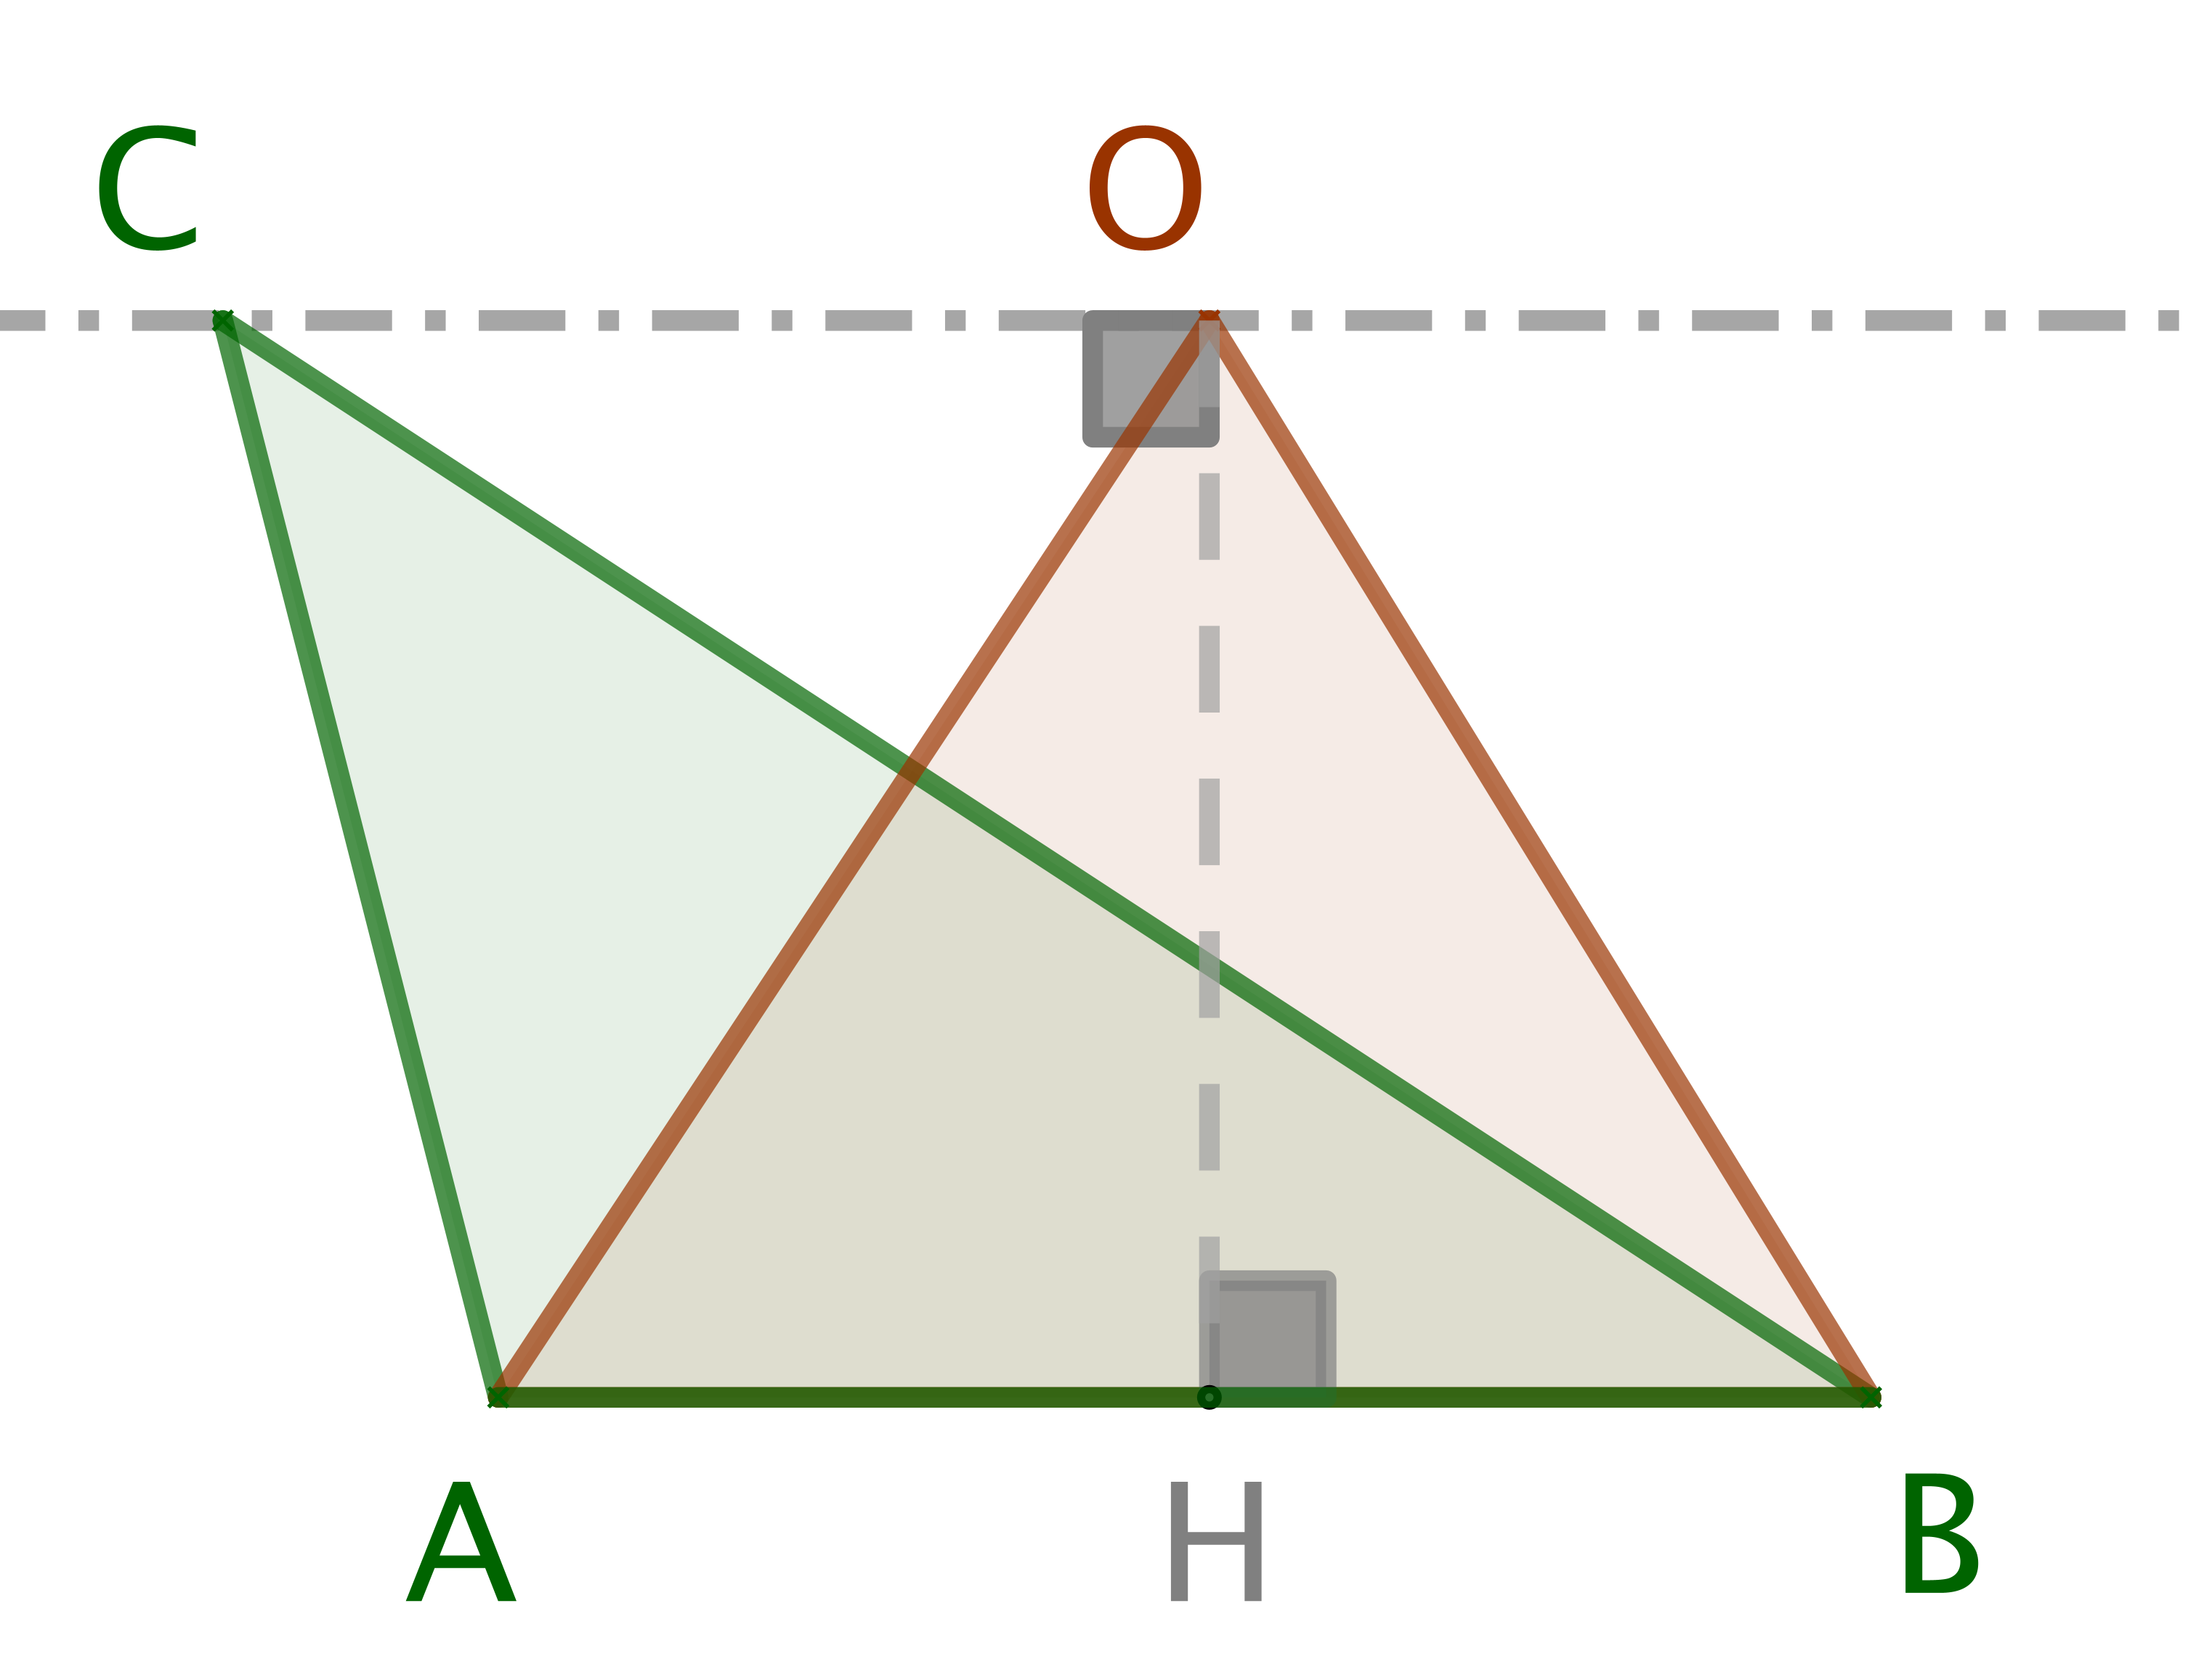
\includegraphics[scale=.4]{content/triangle-one-side-fixed/triangle.png}
	\end{center}

	
	Via une symétrie axiale, voir ci-dessous, il est aisé de noter que $\perim{ABC} \geq \perim{ABO}$, avec égalité uniquement si $ABC$ est isocèle en $C$.
	Plus précisément, en passant de $C$ à $O$, le périmètre diminue.
	
	\begin{center}
		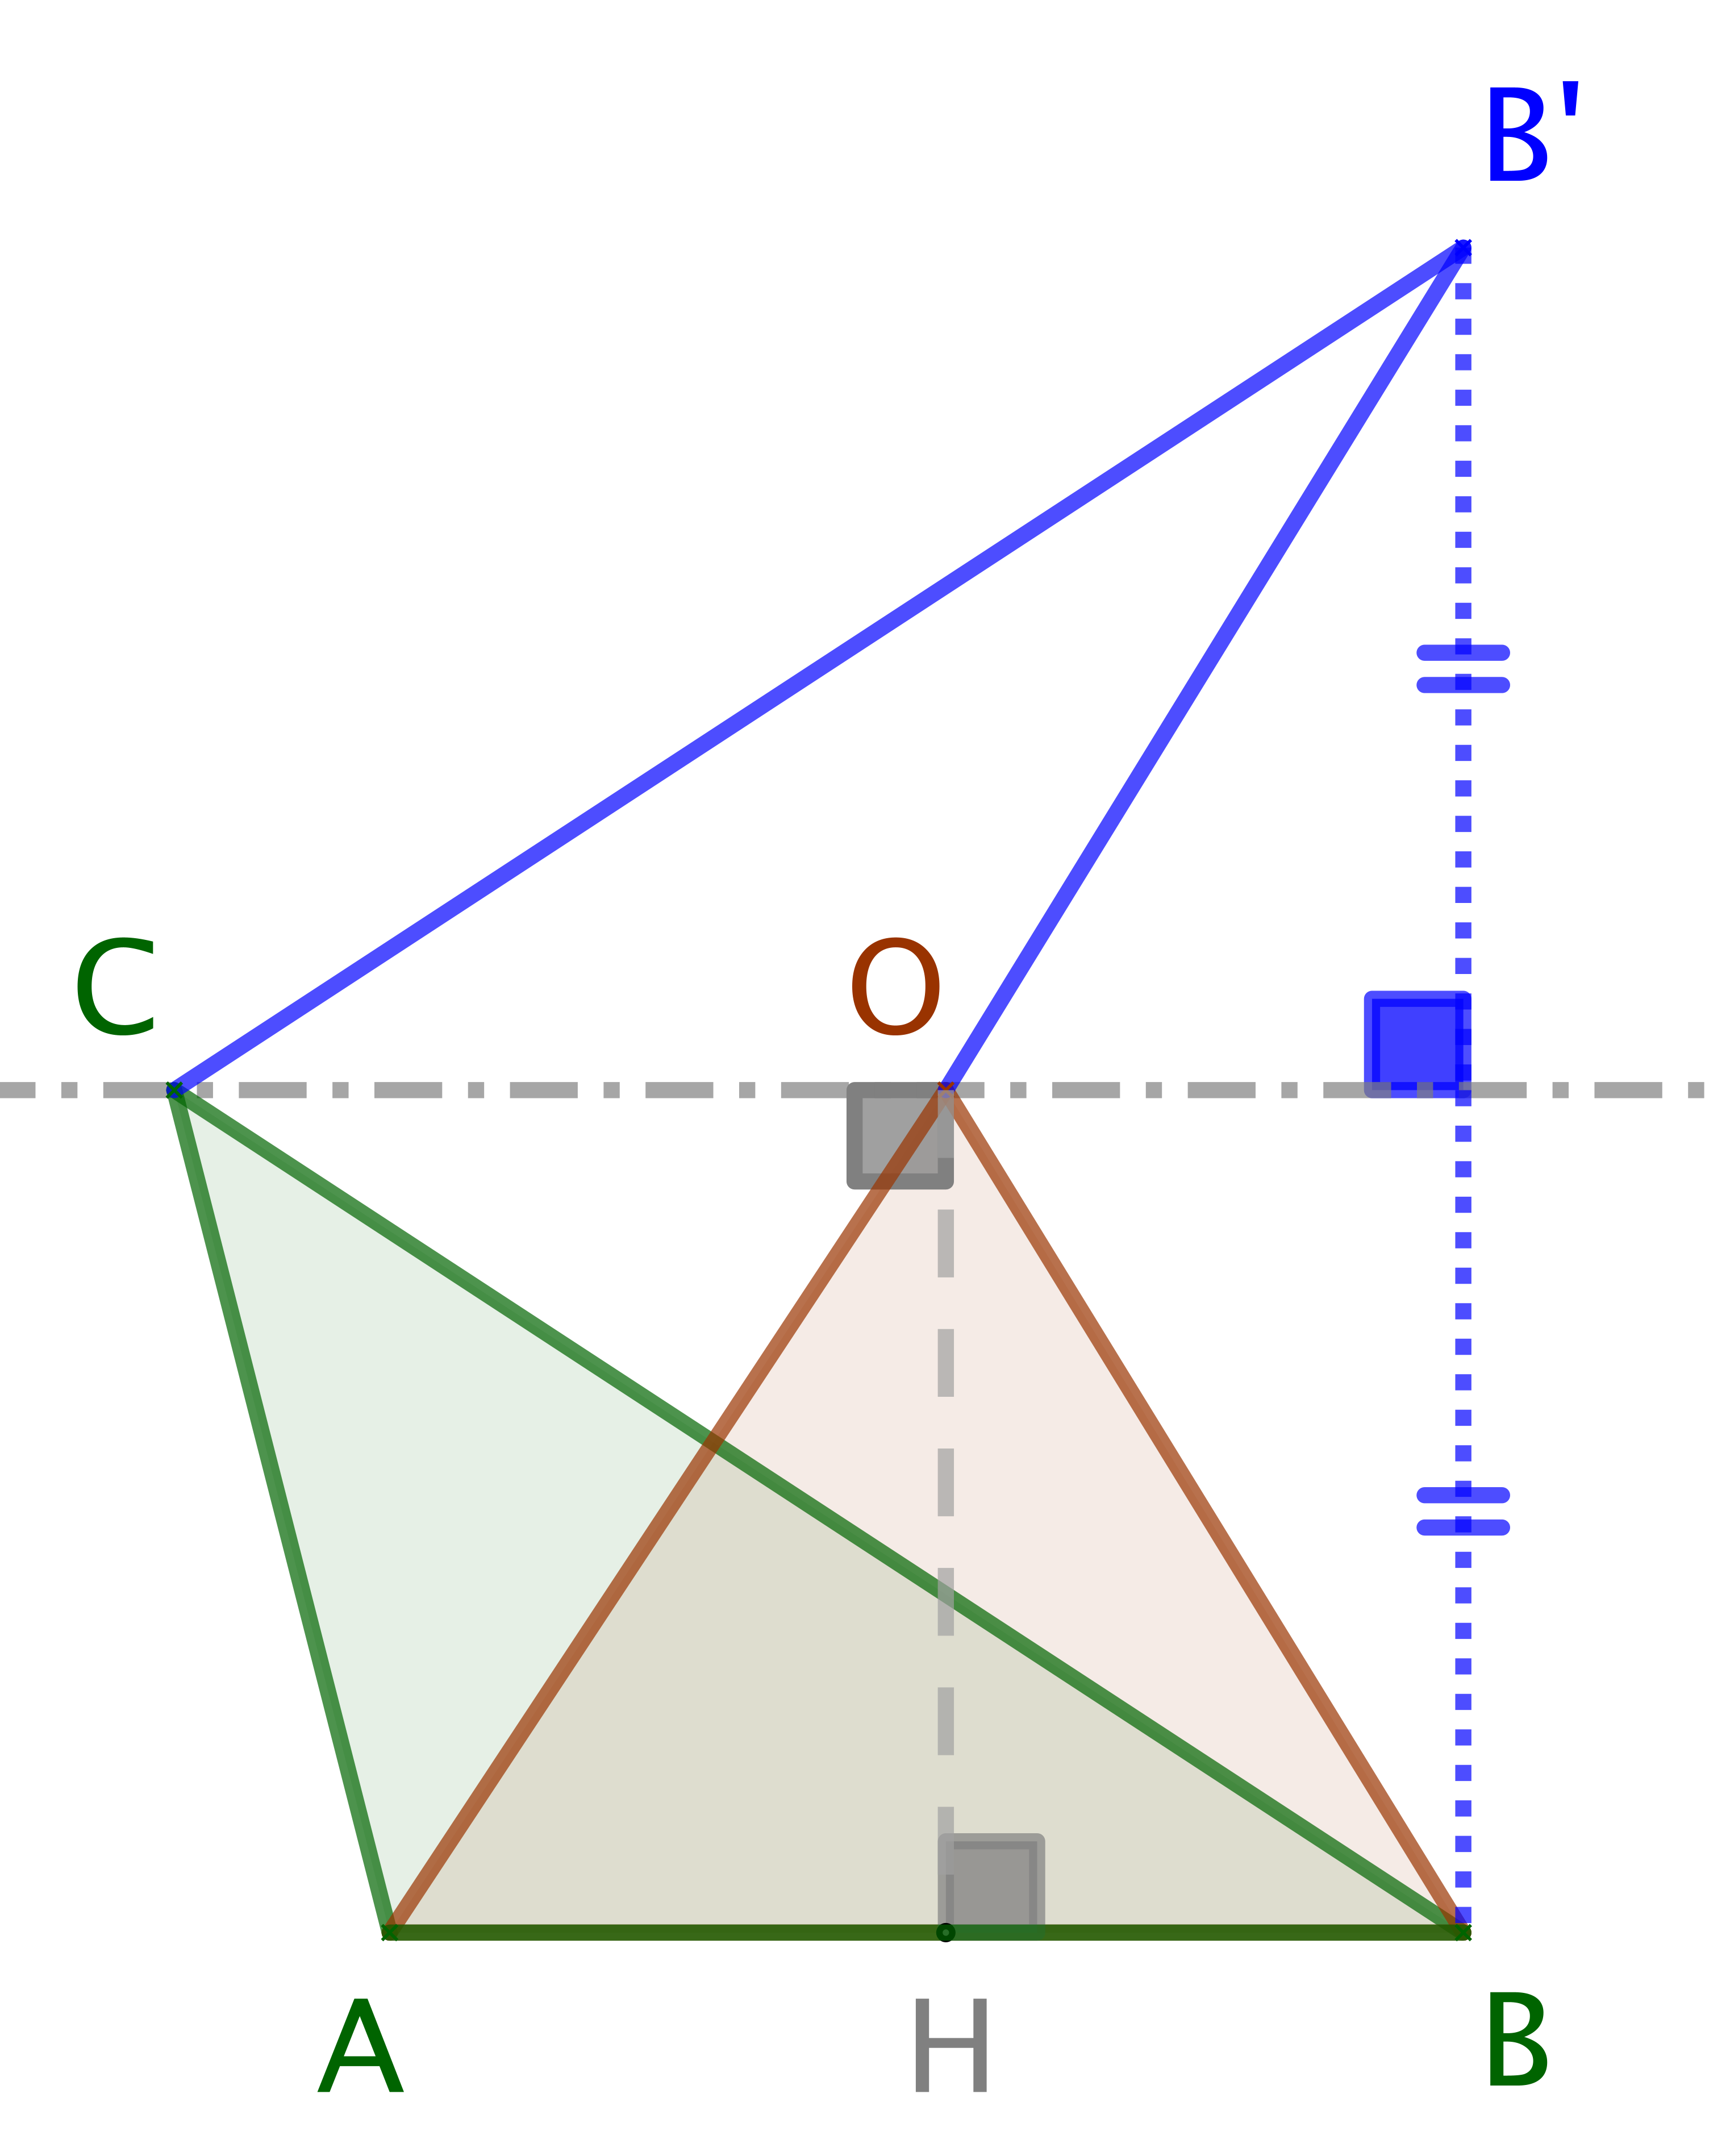
\includegraphics[scale=.4]{content/triangle-one-side-fixed/proof.png}
	\end{center}
	
	Une dilatation \focus{verticale} de rapport $r = \frac{\perim{ABC}}{\perim{ABO}} \geq 1$ donne un triangle isocèle $ABO^{\,\prime}$ tel que 
	$\perim{ABO^{\,\prime}} = p$
	et 
	$\area{ABO^{\,\prime}} \geq \area{ABC}$, avec égalité uniquement si $ABC$ est isocèle en $C$. 
	Contrat rempli!%
	\footnote{
		Dans la section \ref{constrained-extrema} est expliqué comment employer la méthode des extrema liés. 
		Les arguments fournis à cet endroit s'adaptent facilement au cas des triangles de base fixée.
	}
\end{proof}


% ----------------------- %


\begin{remark}
	La recherche parmi les triangles avec un côté fixé de celui ayant un périmètre minimal pour une aire fixée est le problème dual de l'isopérimétrie pour ces triangles.
\end{remark}

%
%
%\subsection{Le cas général}
%\begin{fact} \label{iso-tri}
	Considérons tous les triangles de périmètre fixé $p$. Parmi tous ces triangles, un seul est d'aire maximale, c'est le triangle équilatéral de côté $c = \dfrac13 p$.
\end{fact}


\begin{proof}	
	Nous allons donner une démonstration constructive via une application itérative du fait \ref{tri-one-side-fixed} qui va donner à la limite le triangle équilatéral d'aire maximale, et ceci avec une vitesse de convergence exponentielle.%
	\footnote{
		Ceci ne va nécessiter que l'emploi de propriétés simples de l'ensemble des réels.
	}
	Partons donc d'un triangle $ABC$ quelconque, mais de périmètre $p$, le fait \ref{tri-one-side-fixed} nous donne successivement les triangles $ACD$, $ADE$ et $AEF$ isocèles en $D$, $E$ et $F$ respectivement, ayant tous pour périmètre $p$, et ceci avec des aires de plus en plus grandes.  
	Le dessin suivant amène à conjecturer qu'en poursuivant le procédé pour avoir ensuite un triangle $AFG$ isocèle en $G$...\,, nous aboutirons \focus{à la limite} à un triangle équilatéral.

	\begin{center}
		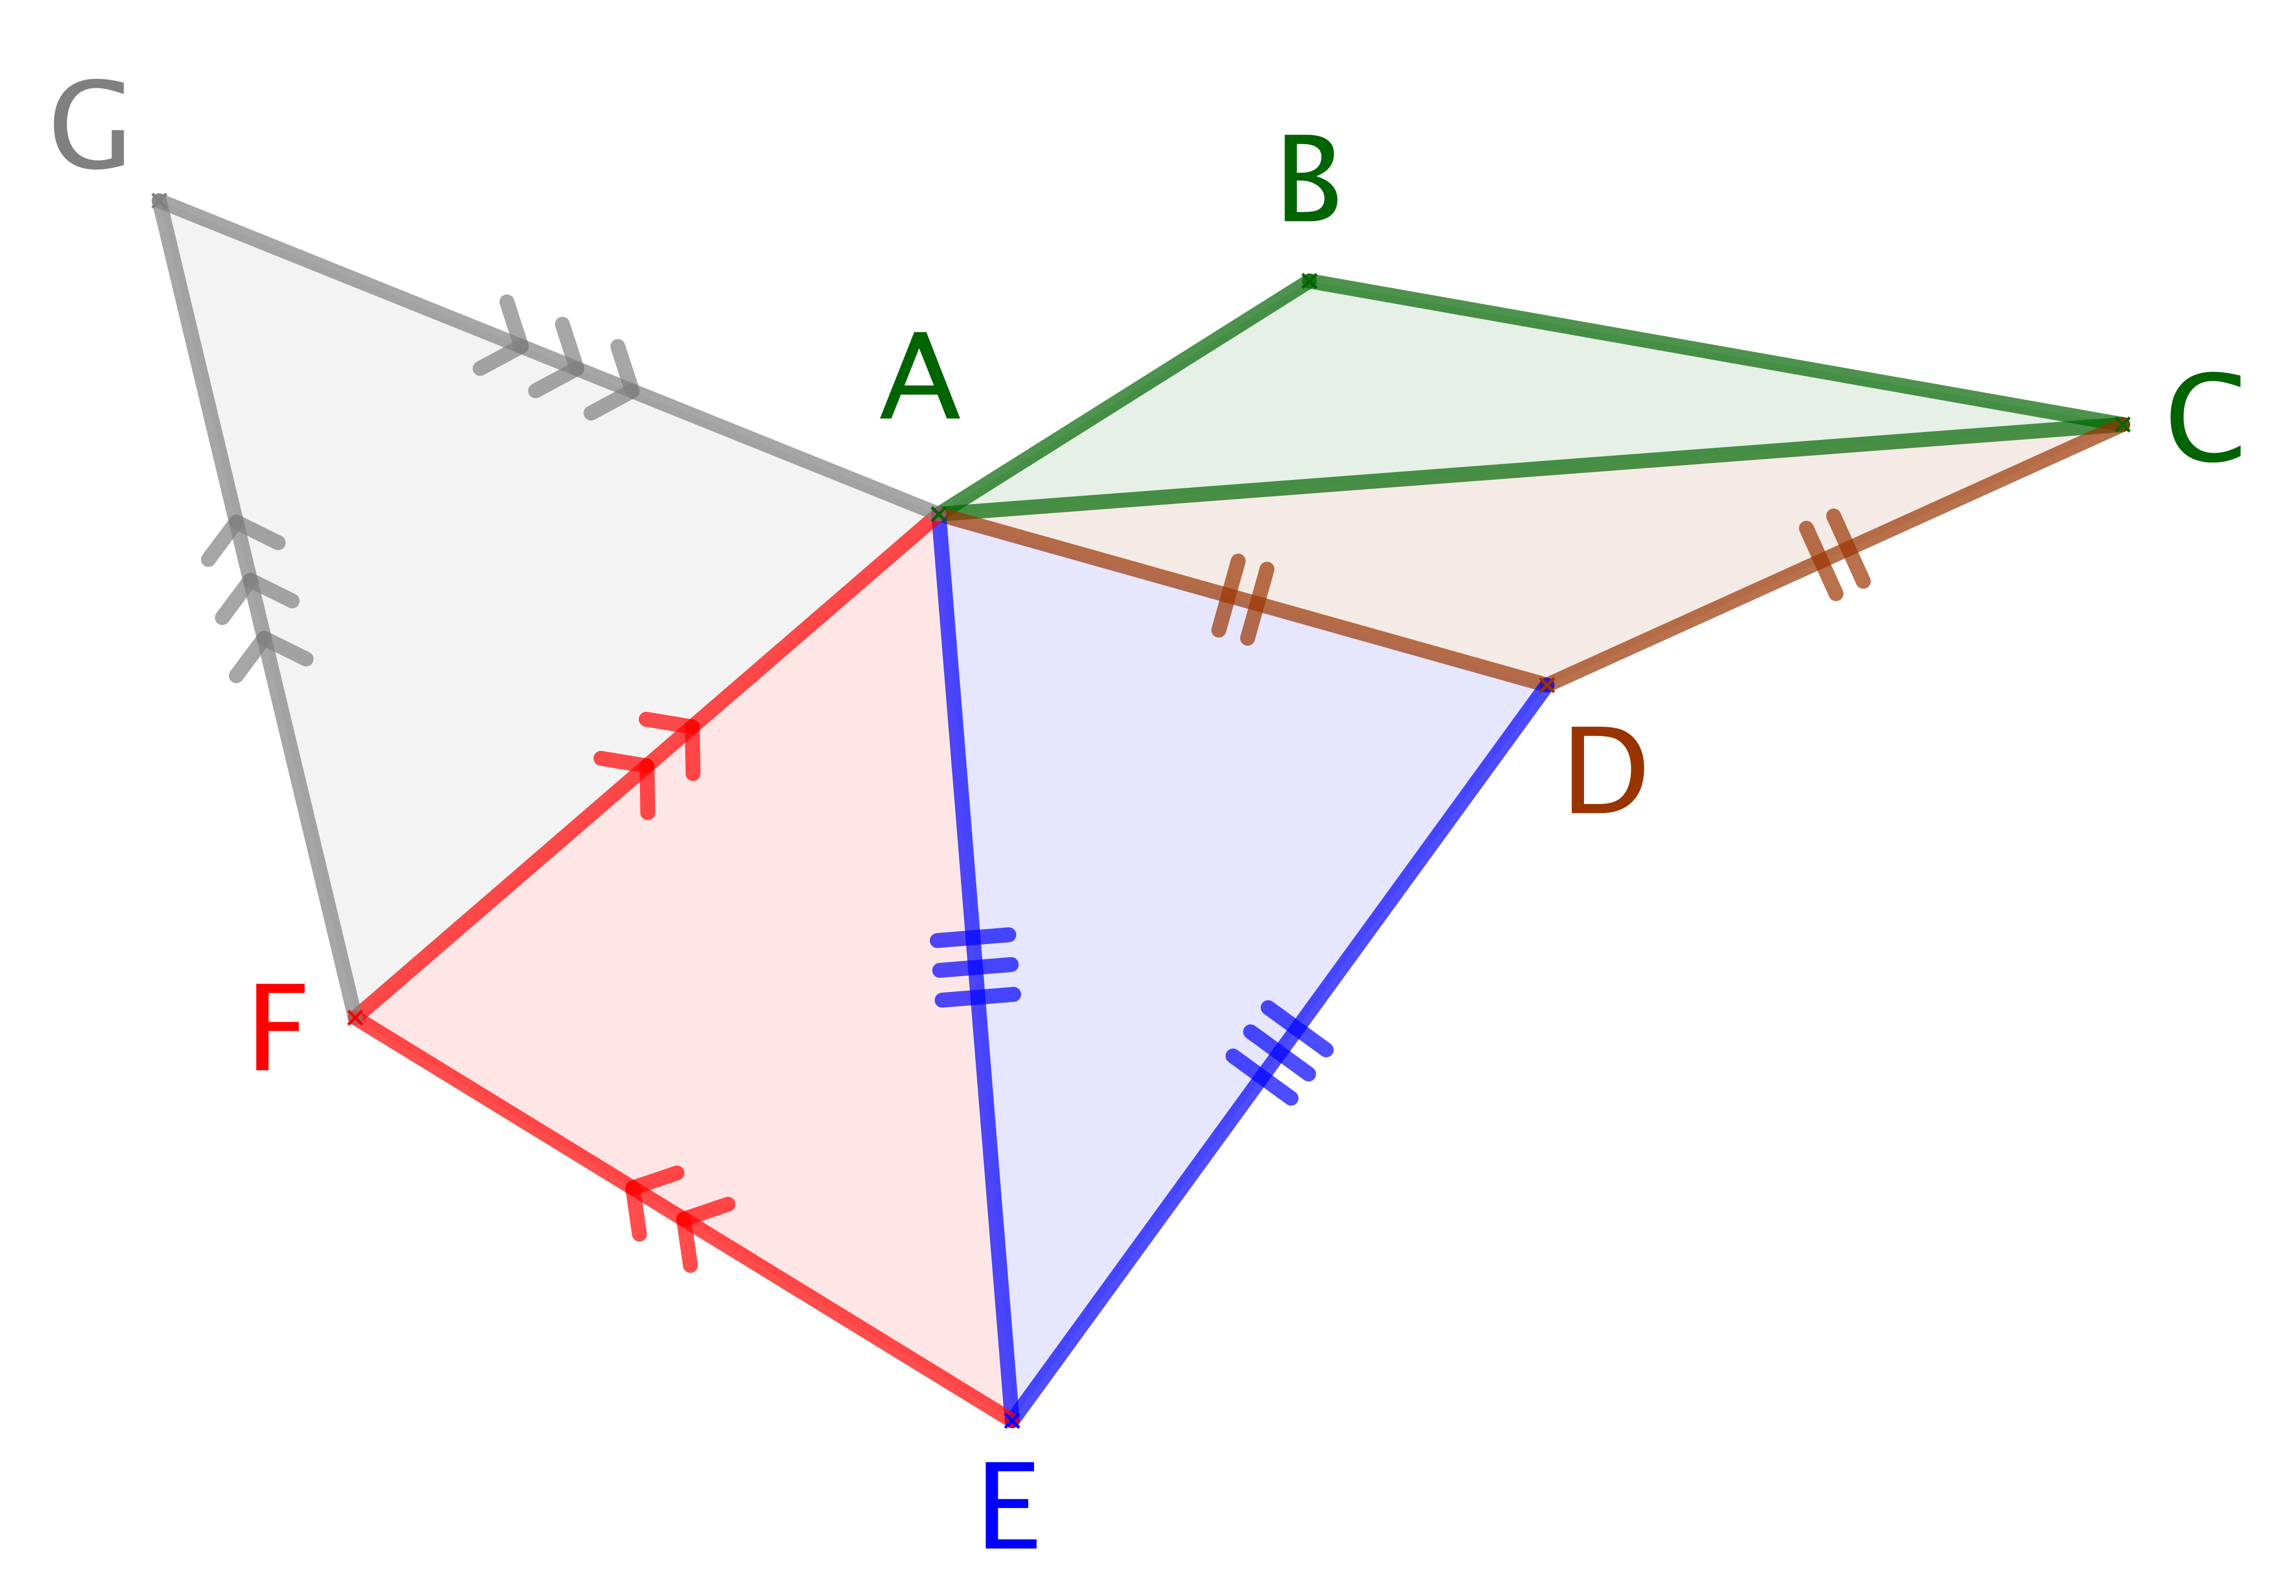
\includegraphics[scale=.4]{content/triangle-gene/proof.png}
	\end{center} 

	
	Le passage d'un triangle quelconque $ABC$ au triangle $ACD$ isocèle en $D$ nous amène à nous concentrer sur ce que donne notre procédé d'agrandissement d'aire à périmètre fixé pour des triangles isocèles. 
	Voici ce que nous pouvons affirmer en supposant $AC > AD$, comme dans notre exemple (nous allons voir que cette hypothèse est sans conséquence).
	%
	\begin{enumerate}
		\item Comme $AC + 2 AD = p$ et $AC > AD$, nous avons $AC > \frac13 p > AD$.
		À l'étape suivante, comme $AD + 2 AE = p$, nous obtenons $AD < \frac13 p < AE$.


		\item Pour $AEF$ isocèle en $F$, comme $AE + 2AF = p$, nous arrivons à  $AE > \frac13 p > AF$.
		
		
		\item \label{tri-equi-conv}
		Tentons de quantifier les écarts à la mesure pivot $p^{\,\prime} = \frac13 p$. 
		%
		\begin{itemize}
			\item Dans $ACD$, posant $AD = p^{\,\prime} - \epsilon_1$, nous avons $AC = p^{\,\prime} + 2 \epsilon_1$.

			\item Dans $ADE$, posant $AE = p^{\,\prime} + \epsilon_2$, nous avons $AD = p^{\,\prime} - 2 \epsilon_2$.

			\item Dans $AEF$, posant $AF = p^{\,\prime} - \epsilon_3$, nous avons $AE = p^{\,\prime} + 2 \epsilon_3$.

			\item Dans $AFG$, posant $AG = p^{\,\prime} + \epsilon_4$, nous avons $AF = p^{\,\prime} - 2 \epsilon_4$.

			\item Donc
			$\epsilon_2 = \frac12 \epsilon_1$,
			$\epsilon_3 = \frac12 \epsilon_2$
			et
			$\epsilon_4 = \frac12 \epsilon_3$.
		\end{itemize}
	\end{enumerate}


	\smallskip
	
	Voici les enseignements de ce qui précède en partant d'un triangle $ABC$ non équilatéral.
	%
	\begin{itemize}
		\item Si $AC = \frac13p$, dès la 1\iere\ itération, nous avons un triangle équilatéral d'aire plus grande.
		
		
		\item Si $AC \neq \frac13p$, notre procédé n'arrivera jamais en un nombre fini d'étapes à un triangle équilatéral.
		Dans ce cas, le point \ref{tri-equi-conv} ci-dessus nous donne une convergence exponentielle des longueurs des côtés vers $p^{\,\prime} = \frac13 p$, tout en ayant des aires des plus en plus grandes.
	\end{itemize}
	
	Dans tous les cas, l'aire d'un triangle non équilatéral de périmètre $p$ est strictement majorée par celle du triangle équilatéral de périmètre $p$. Et tout ceci a été obtenu via de la géométrie et de l'analyse élémentaires!
\end{proof}

%
%
\subsection{Des preuves courtes non géométriques}
\leavevmode

\smallskip

Nous donnons ici des preuves courtes du fait \ref{iso-tri}, mais sans notion géométrique intuitive. Efficacité versus beauté, l'auteur a choisi son camp depuis longtemps !


% ----------------------- %


\begin{proof}[\altproof{1}]
	Selon \textbf{la formule de Héron},
	$\sqrt{s(s - a)(s - b)(s - c)}$
	est l'aire d'un triangle de côtés $a$, $b$, $c$ et de demi-périmètre $s = \num{.5} p$.
	La comparaison des moyennes géométrique et arithmétique%
	\footnote{
		La formule de Héron reste un argument géométrique, mais quid de la comparaison des moyennes géométrique et arithmétique d'ordre $3$, généralement justifiée via la concavité de la fonction logarithme.
		À l'ordre $2$, l'inégalité s'obtient aisément par un argument géométrique simple: voir la remarque \ref{ineq-geo-quad-arith}.
	}
	donne
	$\sqrt[3]{(s - a)(s - b)(s - c)} \leq \frac13 \big( (s - a) + (s - b) + (s - c) \big)$,
	puis
	$s(s - a)(s - b)(s - c) \leq \frac{1}{27} s^4$,
	et enfin
	$\sqrt{s(s - a)(s - b)(s - c)} \leq \frac{p^2}{12 \sqrt{3}}$
	où $\frac{p^2}{12 \sqrt{3}}$ est l'aire du triangle équilatéral de périmètre $p$.
\end{proof}


% ----------------------- %


\begin{proof}[\altproof{2}]
	Faisons appel à \textbf{l'analyse élémentaire aidée du fait \ref{tri-one-side-fixed}}.
	Ce fait permet de se concentrer sur $ABC$ isocèle en $C$. 
	Choisissons un repère orthonormé $\pvaxes{O | i | j}$ tel que  $A\coord{0 | 0}$, $B\coord{AB | 0}$ et $C\coord{x_C | y_C}$ avec $y_C \geq 0$, et posons $c = AC = BC \neq 0$ et $s = \frac{p}{2}$.
	Donc
	$x_B = 2 s - 2 c \neq 0$, et 
	$y_C = \sqrt{c^2 - (s - c)^2}$, 
	puis
	$\area{ABC}^2 = (s - c)^2 (c^2 - (s - c)^2 )$,
	soit
	$\area{ABC}^2 = s (s - c)^2 (s - 2 c)$.%
	\footnote{
		Nous venons de démontrer la formule de Héron dans le cas particulier d'un triangle isocèle.
	}
	Or, le maximum de la fonction 
	$\alpha : c \mapsto s (s - c)^2 (s - 2 c)$ est forcément atteint en $c$ annulant 
	$\sder{\alpha}{1}(c) = - 2 s (s - c) (s - 2 c) - 2 s (s - c)^2 = 2 s (c - s) (2s - 3c)$, 
	soit pour $c = \frac{2s}{3} = \frac{p}{3}$, car $c = s$ est exclu,
	donc $ABC$ équilatéral est la solution \og optimale \fg.
\end{proof}


% ----------------------- %


\begin{proof}[\altproof{3}] \label{tri-topo-comp}
	Utilisons \textbf{juste la continuité et la compacité}.% (nous généraliserons cette idée au cas des polygones à $n$ côtés).
	%
	\begin{itemize}
		\item On munit le plan d'un repère orthonormé $\pvaxes{O | i | j}$. 

		\item Les triangles $ABC$ tels que $\perim{ABC} = p$ sont représentés en posant $A\coord{0 | 0}$, $B\coord{AB | 0}$ et $C\coord{x_C | y_C}$ avec $y_C \geq 0$. Un triangle peut donc avoir trois représentations, mais peu importe.
		De plus, on accepte les triangles dégénérés pour lesquels nous avons $x_B = 0$ ou $y_C = 0$ dans notre représentation.
		Nous notons alors $\setproba{T} \subset \RR^3$ l'ensemble des triplets $\coord{x_B | x_C | y_C}$ ainsi obtenus.

		\item Il est facile de justifier que $\setproba{T}$ est séquentiellement fermé dans $\RR^3$.
		De plus, $\setproba{T}$ est borné car $x_B$, $x_C$ et $y_C$ le sont.
		En résumé, $\setproba{T}$ est un compact de $\RR^3$.

		\item La fonction $\alpha: \coord{x_B | x_C | y_C} \in \setproba{T} \mapsto \num{.5} x_B y_C \in \RRp$ est la fonction \onedef{aire} des triangles représentés.
		Par continuité et compacité, $\alpha$ admet un maximum sur $\setproba{T}$. 
		

		\item Notons $ABC$ un triangle maximisant $\alpha$.
		Forcément, $ABC$ n'est pas dégénéré. 
		Le fait \ref{tri-one-side-fixed} implique que $ABC$ est équilatéral. 
		En effet,
		dans le cas contraire, il existe un sommet $X$ en lequel $ABC$ n'est pas isocèle, mais la \og maximalité \fg\ de $ABC$ contredit le fait \ref{tri-one-side-fixed} en considérant comme fixé le côté opposé au sommet $X$.
	\end{itemize}
	
	\null\vspace{-6ex}
\end{proof}


% ----------------------- %


\begin{proof}[\altproof{4}] \label{constrained-extrema}
	Nous allons faire appel à \textbf{la méthode des extrema liés et la formule de Héron}.
	Pour cela, notons que l'aire d'un triangle étant positive ou nulle, nous pouvons chercher à maximiser son carré
	$f(a;b;c) = s(s - a)(s - b)(s - c)$
%	          = \frac{1}{16} (a + b + c)(b + c - a)(a + c - b)(a + b - c)$,
	sous la contrainte $2s = a + b + c$ où $s = \num{.5} p > 0$ est constant.
	Notant $g(a;b;c) = a + b + c - 2 s$, la contrainte s'écrit $g(a;b;c) = 0$.
	%
	\begin{itemize}
		\item Si un extremum existe,
    	$\exists \lambda \in \RR$ tel que
    	$\pder[i]{f}{a}{1} = \lambda \pder[i]{g}{a}{1}$,
    	$\pder[i]{f}{b}{1} = \lambda \pder[i]{g}{b}{1}$ et
    	$\pder[i]{f}{c}{1} = \lambda \pder[i]{g}{c}{1}$
		d'après la méthode des extrema liés.

		\item Donc
		$- s(s - b)(s - c) = - s(s - a)(s - c) = - s(s - a)(s - b)$,
		et par conséquent
		$(s - b)(s - c) = (s - a)(s - c) = (s - a)(s - b)$.

		\item Les cas $s = a$, $s = b$ et $s = c$ donnent $f(a;b;c) = 0$.

		\item Le cas $\big[ s \neq a, s \neq b \text{ et } s \neq c \big]$ n'est envisageable que si $a = b = c = \frac{p}{3}$, ceci impliquant $f(a;b;c) = \frac{1}{16} p \big( \frac{p}{3} \big)^3 = \big( \frac{p^2}{12 \sqrt{3}} \big)^2 > 0$.

		\item En résumé, l'existence d'un maximum implique que ce maximum corresponde au cas du triangle équilatéral.

		\item Il reste à démontrer qu'un tel maximum existe pour pouvoir conclure: ceci est facile à justifier en considérant l'ensemble compact $\intervalC{0}{2s}^3$ de $\RR^3$, et la continuité de $f$.
	\end{itemize}
	
	\null\vspace{-6ex}
\end{proof}

%
%
%% ------------- %
%
%
%\section{Quadrilatères}
%
%\subsection{Les rectangles}
%\begin{fact} \label{iso-rect}
	Considérons tous les rectangles de périmètre fixé $p$. Parmi tous ces rectangles, celui d'aire maximale est le carré de côté $c = \num{.25} p$.
\end{fact}


\begin{proof}
	Une preuve courante est d'exprimer l'aire du rectangle comme un polynôme du 2\ieme\ degré en $L$ par exemple.%
	\footnote{
		L'aire est donnée par $L \ell = L (\num{.5} p - L)$ qui est maximale en $L_M = \num{.25} p$ (moyenne des racines), d'où $\ell_M = \num{.25} p = L_M$.
	}
	On peut en fait faire plus simplement grâce au dessin suivant où les rectangles $1$, $2$ et $3$ sont isométriques au rectangle vert étudié de dimension $L \times \ell$.

	\begin{center}
		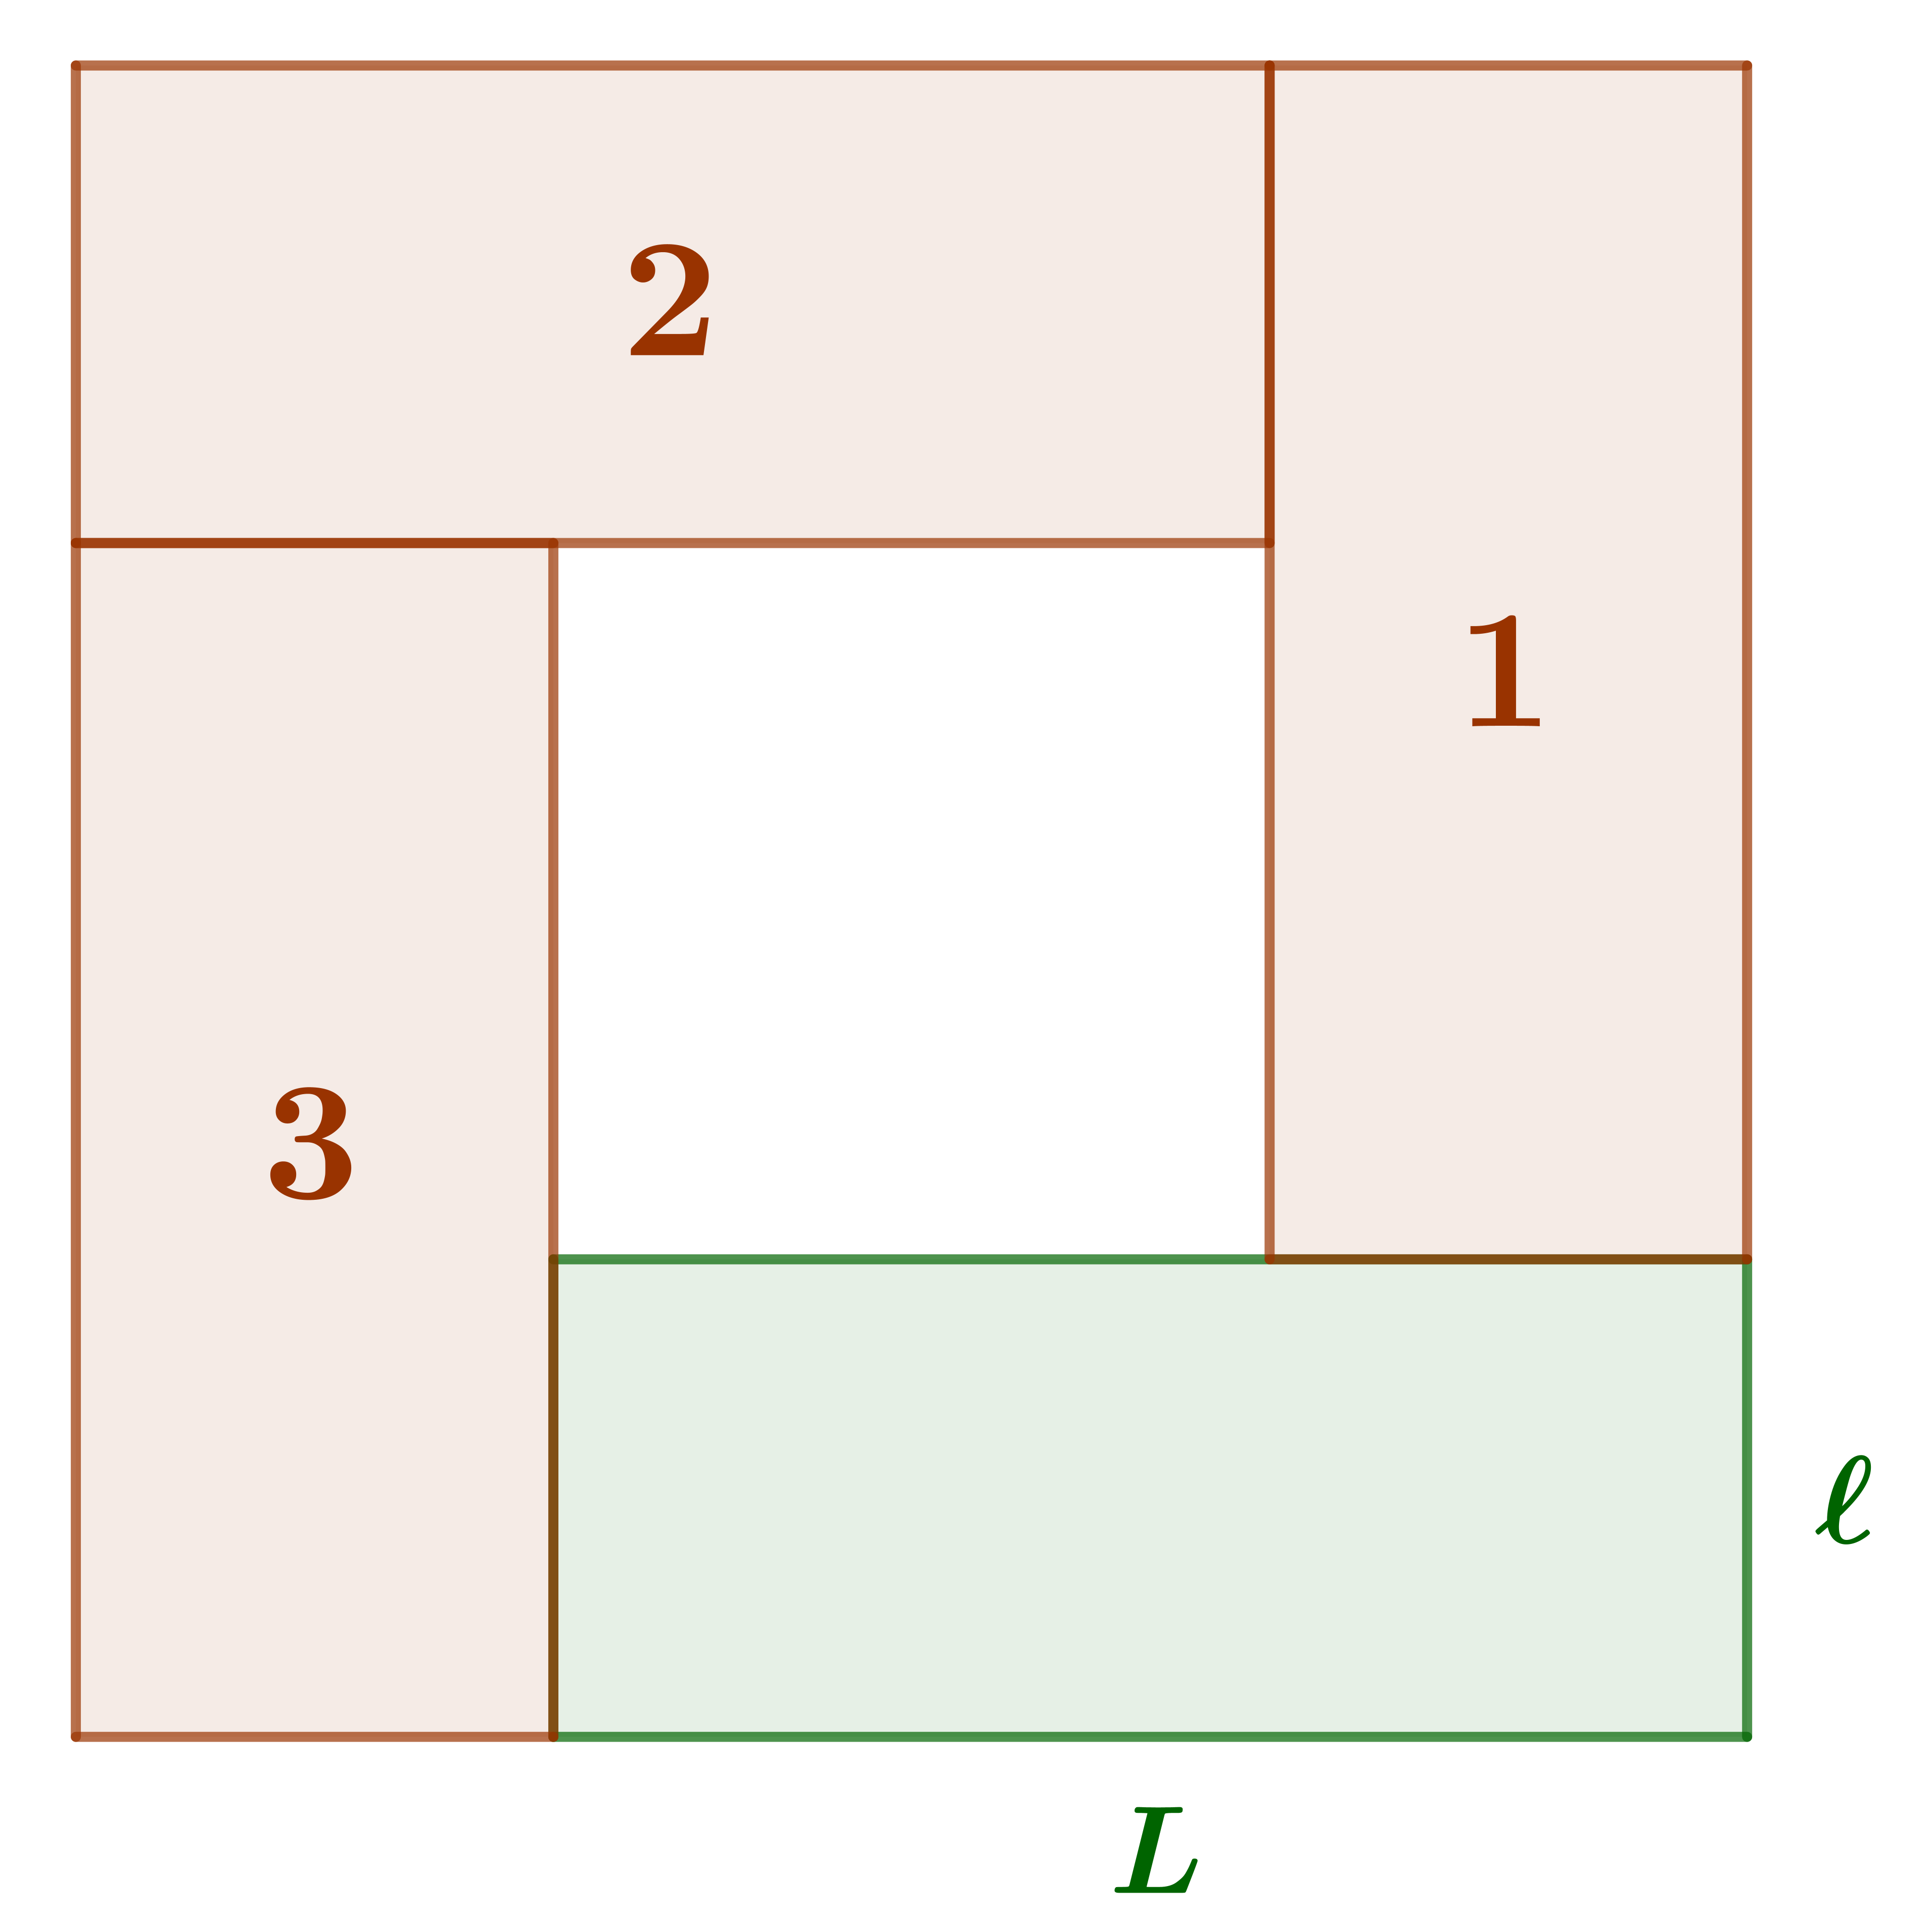
\includegraphics[scale=.4]{content/rectangle/rectangle.png}
	\end{center}
	
	Le raisonnement tient alors aux constations suivantes accessibles à un collégien.
	%
	\begin{enumerate}
		\item Le grand carré a une aire supérieure ou égale à $4 L \ell$.

		\item Le grand carré a un périmètre égal à $4 (L + \ell)$.

		\item Via une homothétie de rapport \num{.5}\,, nous obtenons un carré d'aire supérieure ou égale à $\num{.5}^2 \times 4 L \ell =  L \ell$, et de périmètre égal à $\num{.5} \times 4 (L + \ell) = 2 (L + \ell)$.
	\end{enumerate}
	
	Donc pour tout rectangle de périmètre $p = 2 (L + \ell)$ et d'aire $L \ell$, nous pouvons construire un carré de périmètre identique, mais avec une aire supérieure ou égale à  $L \ell$. Joli! Non?
\end{proof}


\begin{remark}
	Au passage, nous avons pour $(L ; \ell) \in \big( \RRsp \big)^2$, $4 L \ell \leq (L + \ell)^2$, c'est-à-dire $2 L \ell \leq L^2 + \ell^2$, d'où $\sqrt{L \ell} \leq \sqrt{\frac12 (L^2 + \ell^2)}$, soit la comparaison des moyennes géométriques et quadratiques d'ordre $2$.
\end{remark}

%
%
%\subsection{Les parallélogrammes}
%\begin{fact} \label{iso-para}
	Considérons tous les parallélogrammes de périmètre fixé $p$. Parmi tous ces parallélogrammes, un seul est d'aire maximale, c'est le carré de côté $c = \num{.25} p$.
\end{fact}


\begin{proof}
	Le calcul de l'aire d'un parallélogramme, voir le dessin ci-dessous, nous donne 
	$\area{ABCD} = \area{ABHH^{\,\prime}}$ et 
	$\perim{ABCD} \geq \perim{ABHH^{\,\prime}}$, 
	avec égalité uniquement si $ABCD$ est un rectangle. 
	
	\begin{center}
		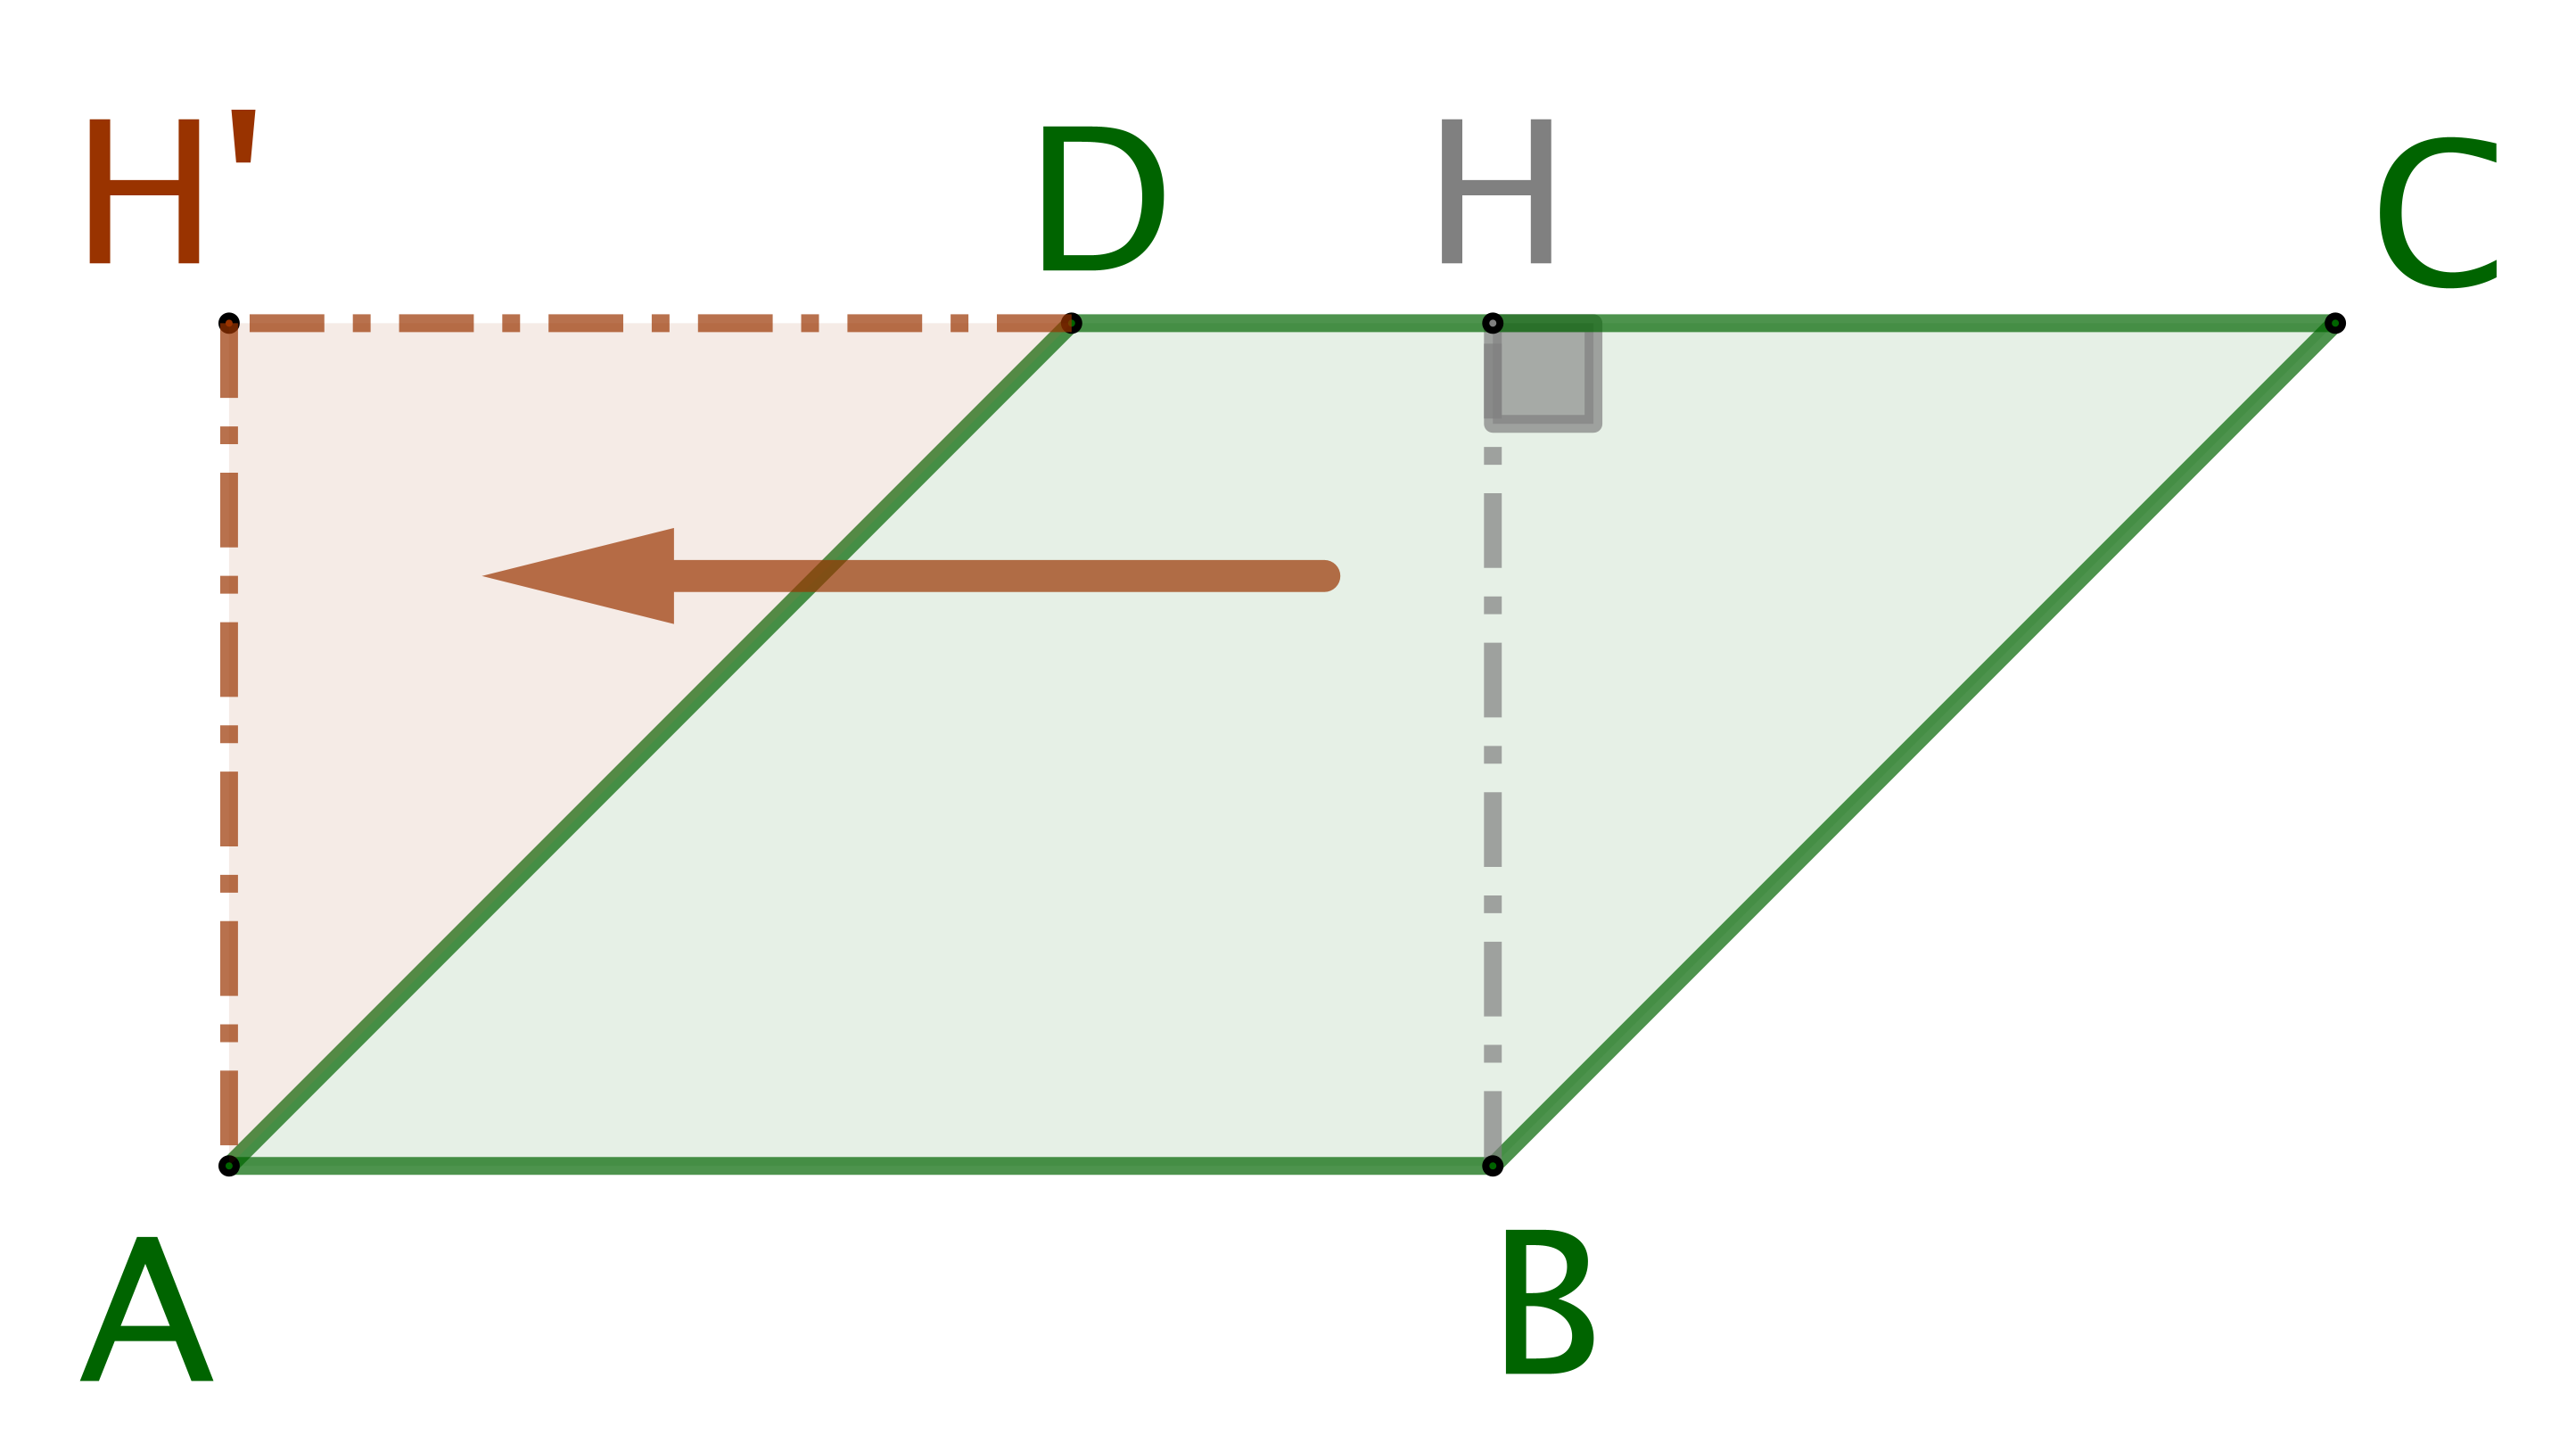
\includegraphics[scale=.4]{content/parallelogram/para-2-rect.png}
	\end{center}
	
	Via une homothétie de rapport $r = \frac{\perim{ABCD}}{\perim{ABHH^{\,\prime}}} \geq 1$, nous obtenons un rectangle 
	de périmètre égal à $p$,
	et d'aire supérieure ou égale à $\area{ABCD}$, 
	avec égalité uniquement si $ABCD$ est un rectangle.
	Nous revenons à la situation du fait \ref{iso-rect} qui permet de conclure très facilement.
\end{proof}


% ----------------------- %


\begin{remark}
	Une méthode analytique devient pénible ici, car il faut, par exemple, prendre en compte l'angle au sommet $A$ du parallélogramme. L'auteur préfère battre en retraite en clôturant cette remarque ici.
%	\footnote{
%		Et oui, l'auteur est un lâche.
%	}
\end{remark}

%
%
%\subsection{Le cas général}
%\begin{fact}
	Considérons tous les quadrilatères de périmètre fixé $p$. Parmi tous ces quadrilatères, celui d'aire maximale est le carré de côté $c = \num{.25} p$.
\end{fact}


\begin{proof}
	La figure suivante montre que pour tout quadrilatère $ABCD$ non convexe en $B$, et de périmètre $p$, il existe un quadrilatère convexe $AB^{\,\prime}CD$ de périmètre $p$, et tel que $\area{AB^{\,\prime}CD} \geq \area{ABCD}$.
	Notre recherche doit donc continuer dans l'ensemble des quadrilatères convexes de périmètre $p$.

	\begin{center}
		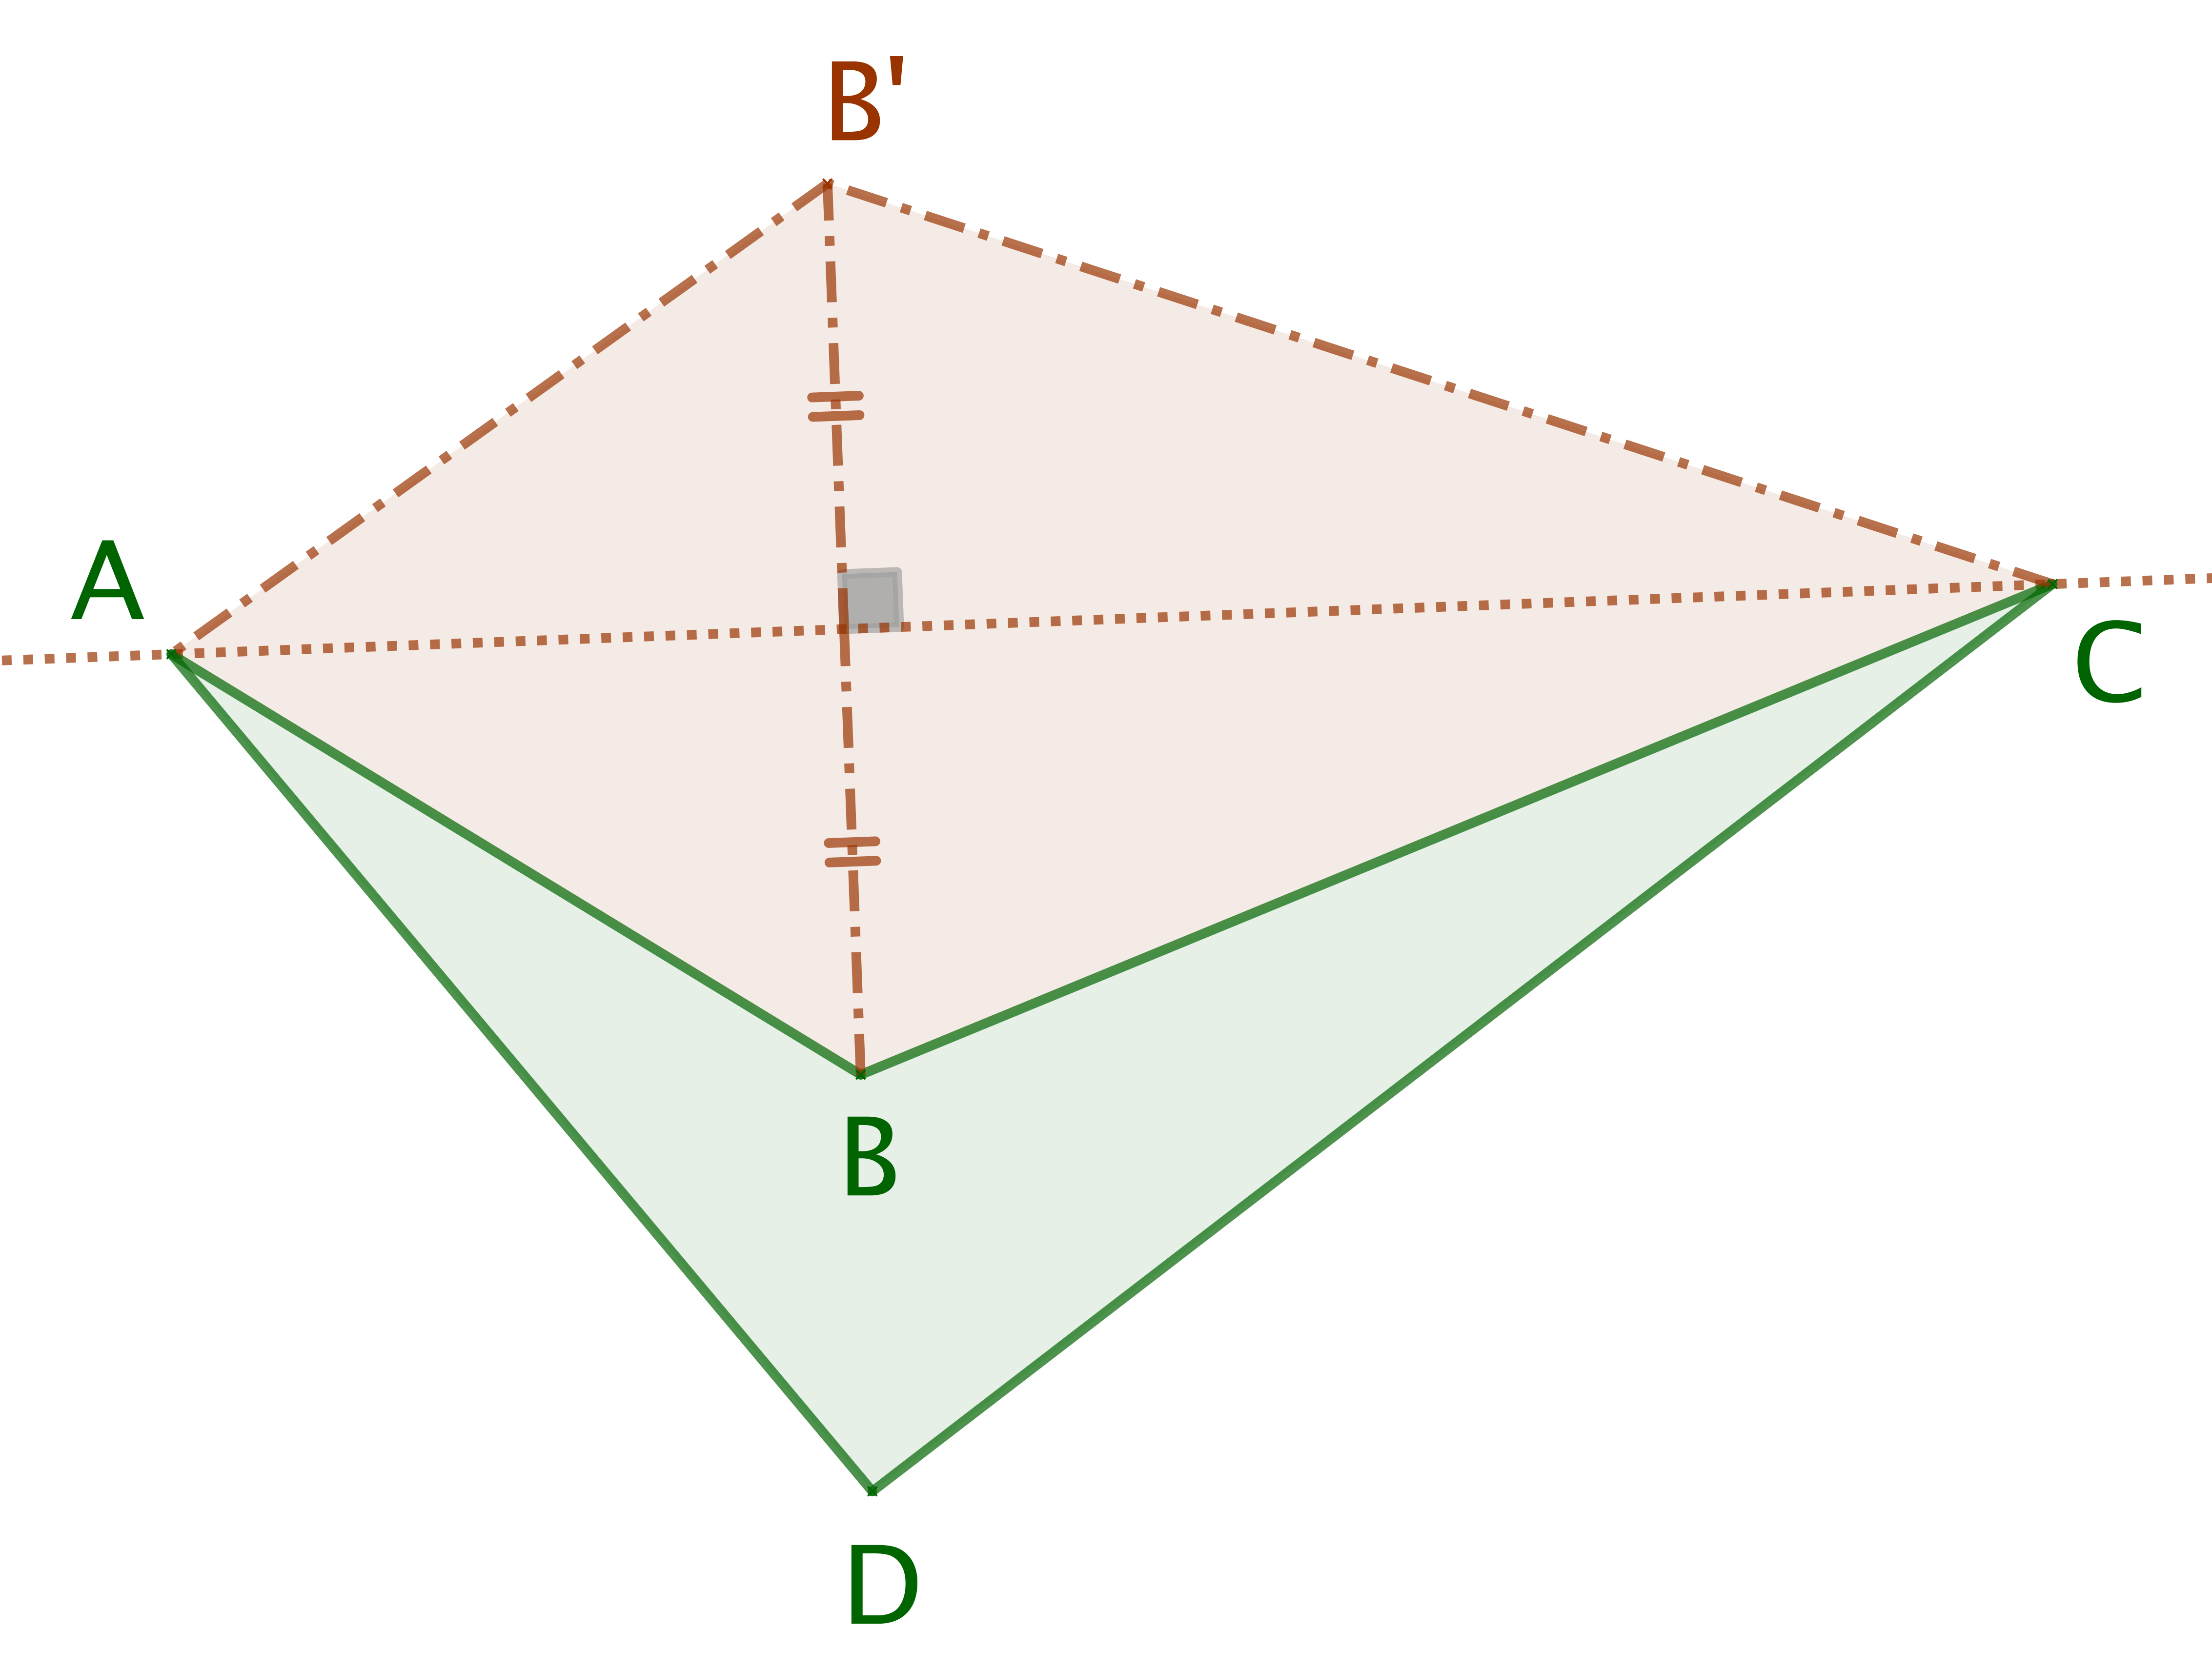
\includegraphics[scale=.4]{content/quadrilateral/quadrilateral-non-convex.png}
	\end{center}
	
	
	Comme dans la preuve du fait \ref{iso-tri-one-side-fixed}, à partir d'un quadrilatère convexe $ABCD$ de périmètre $p$, nous obtenons un quadrilatère convexe $AB^{\,\prime}CD$ de périmètre $p$,%
	\footnote{
		Noter que
		$\perim{AB^{\,\prime}CD} = \perim{AB^{\,\prime}C} + \perim{ACD} - 2 AC$.
	}
	et tel que $AB^{\,\prime} = B^{\,\prime}C$ et $\area{AB^{\,\prime}CD} \geq \area{ABCD}$ comme le montre la figure ci-après. 

	\begin{center}
		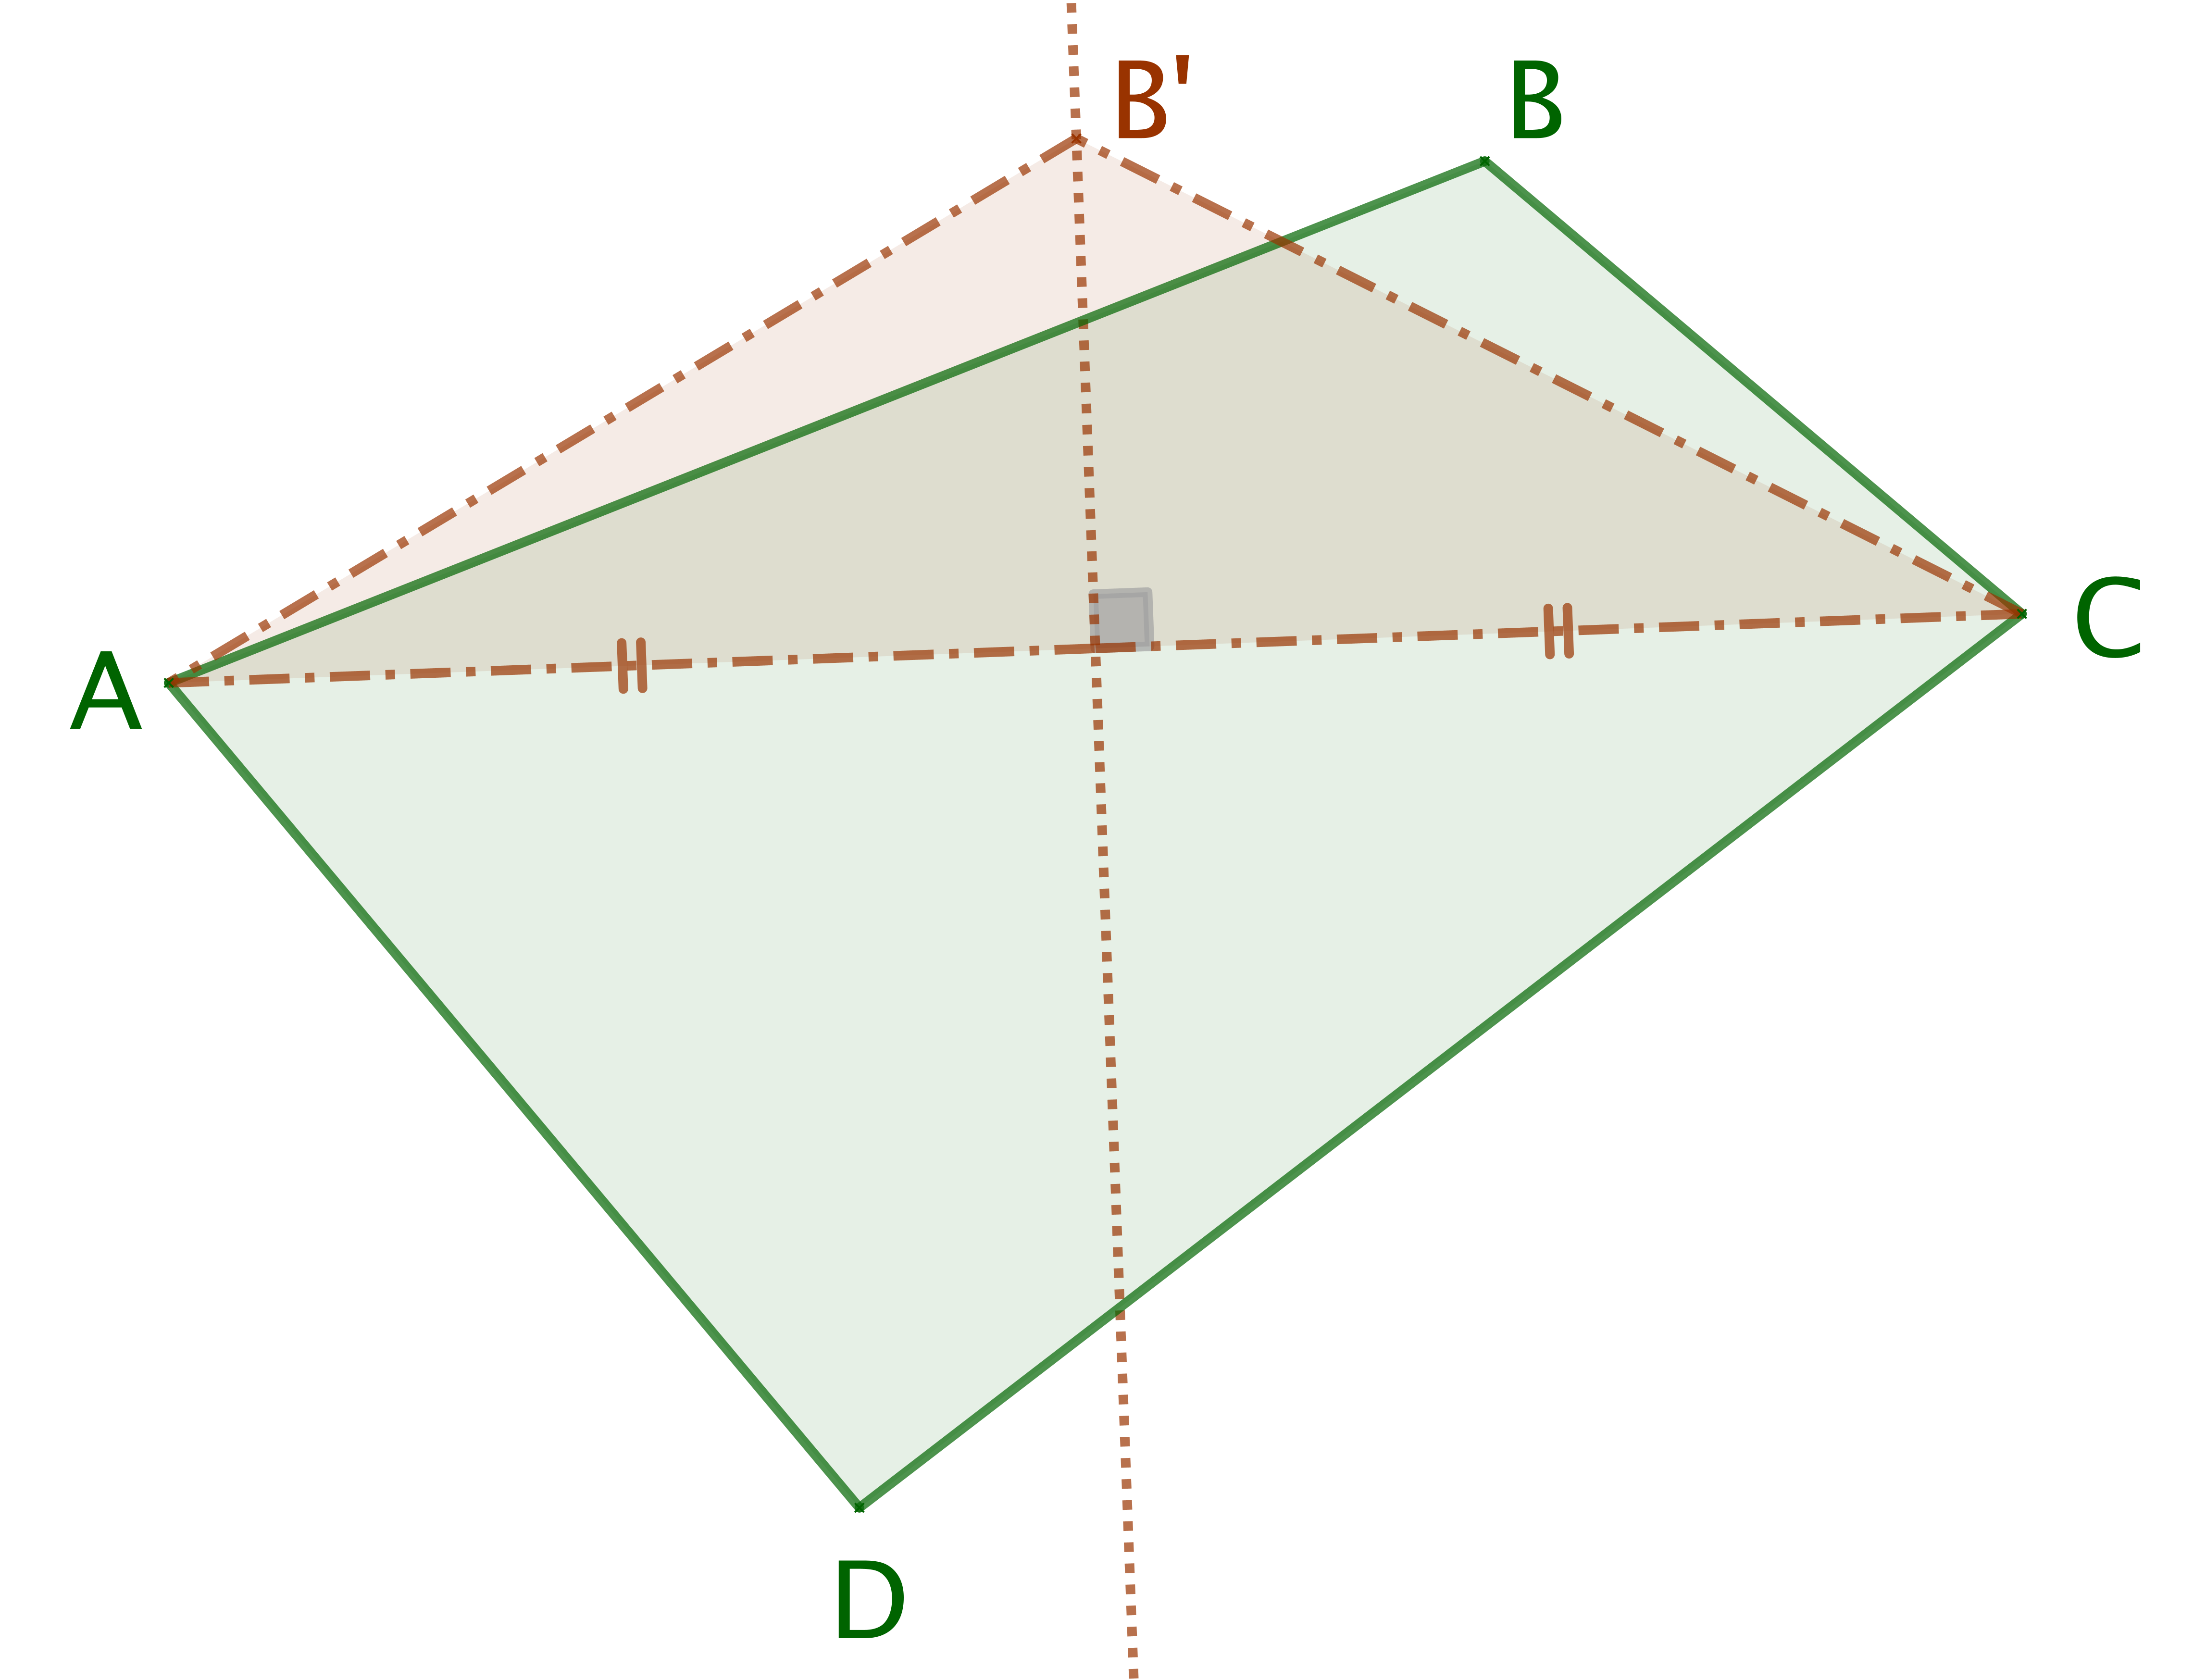
\includegraphics[scale=.4]{content/quadrilateral/quadrilateral-convex-gene.png}
	\end{center}
	
	
	La méthode précédente appliquée au sommet $D$ donne un cerf-volant $ABCD$ de périmètre $p$, et tel que $AB = BC$ et $AD = DC$, voir ci-dessous. 
	Cette même méthode avec les sommets $A$ et $C$ fournit un losange $A^{\,\prime}BC^{\,\prime}D$ de périmètre $p$, et tel que $\area{A^{\,\prime}BC^{\,\prime}D} \geq \area{ABCD}$.
	%
	En effet, nous avons
	$p = 2(AB + AD)$
	et
	$\perim{A^{\,\prime}BD} = \perim{ABD}$,
	donc
	$A^{\,\prime}B = A^{\,\prime}D = \num{.25} p$,
	et de même, nous obtenons
	$C^{\,\prime}B = C^{\,\prime}D = \num{.25} p$.

	\begin{center}
		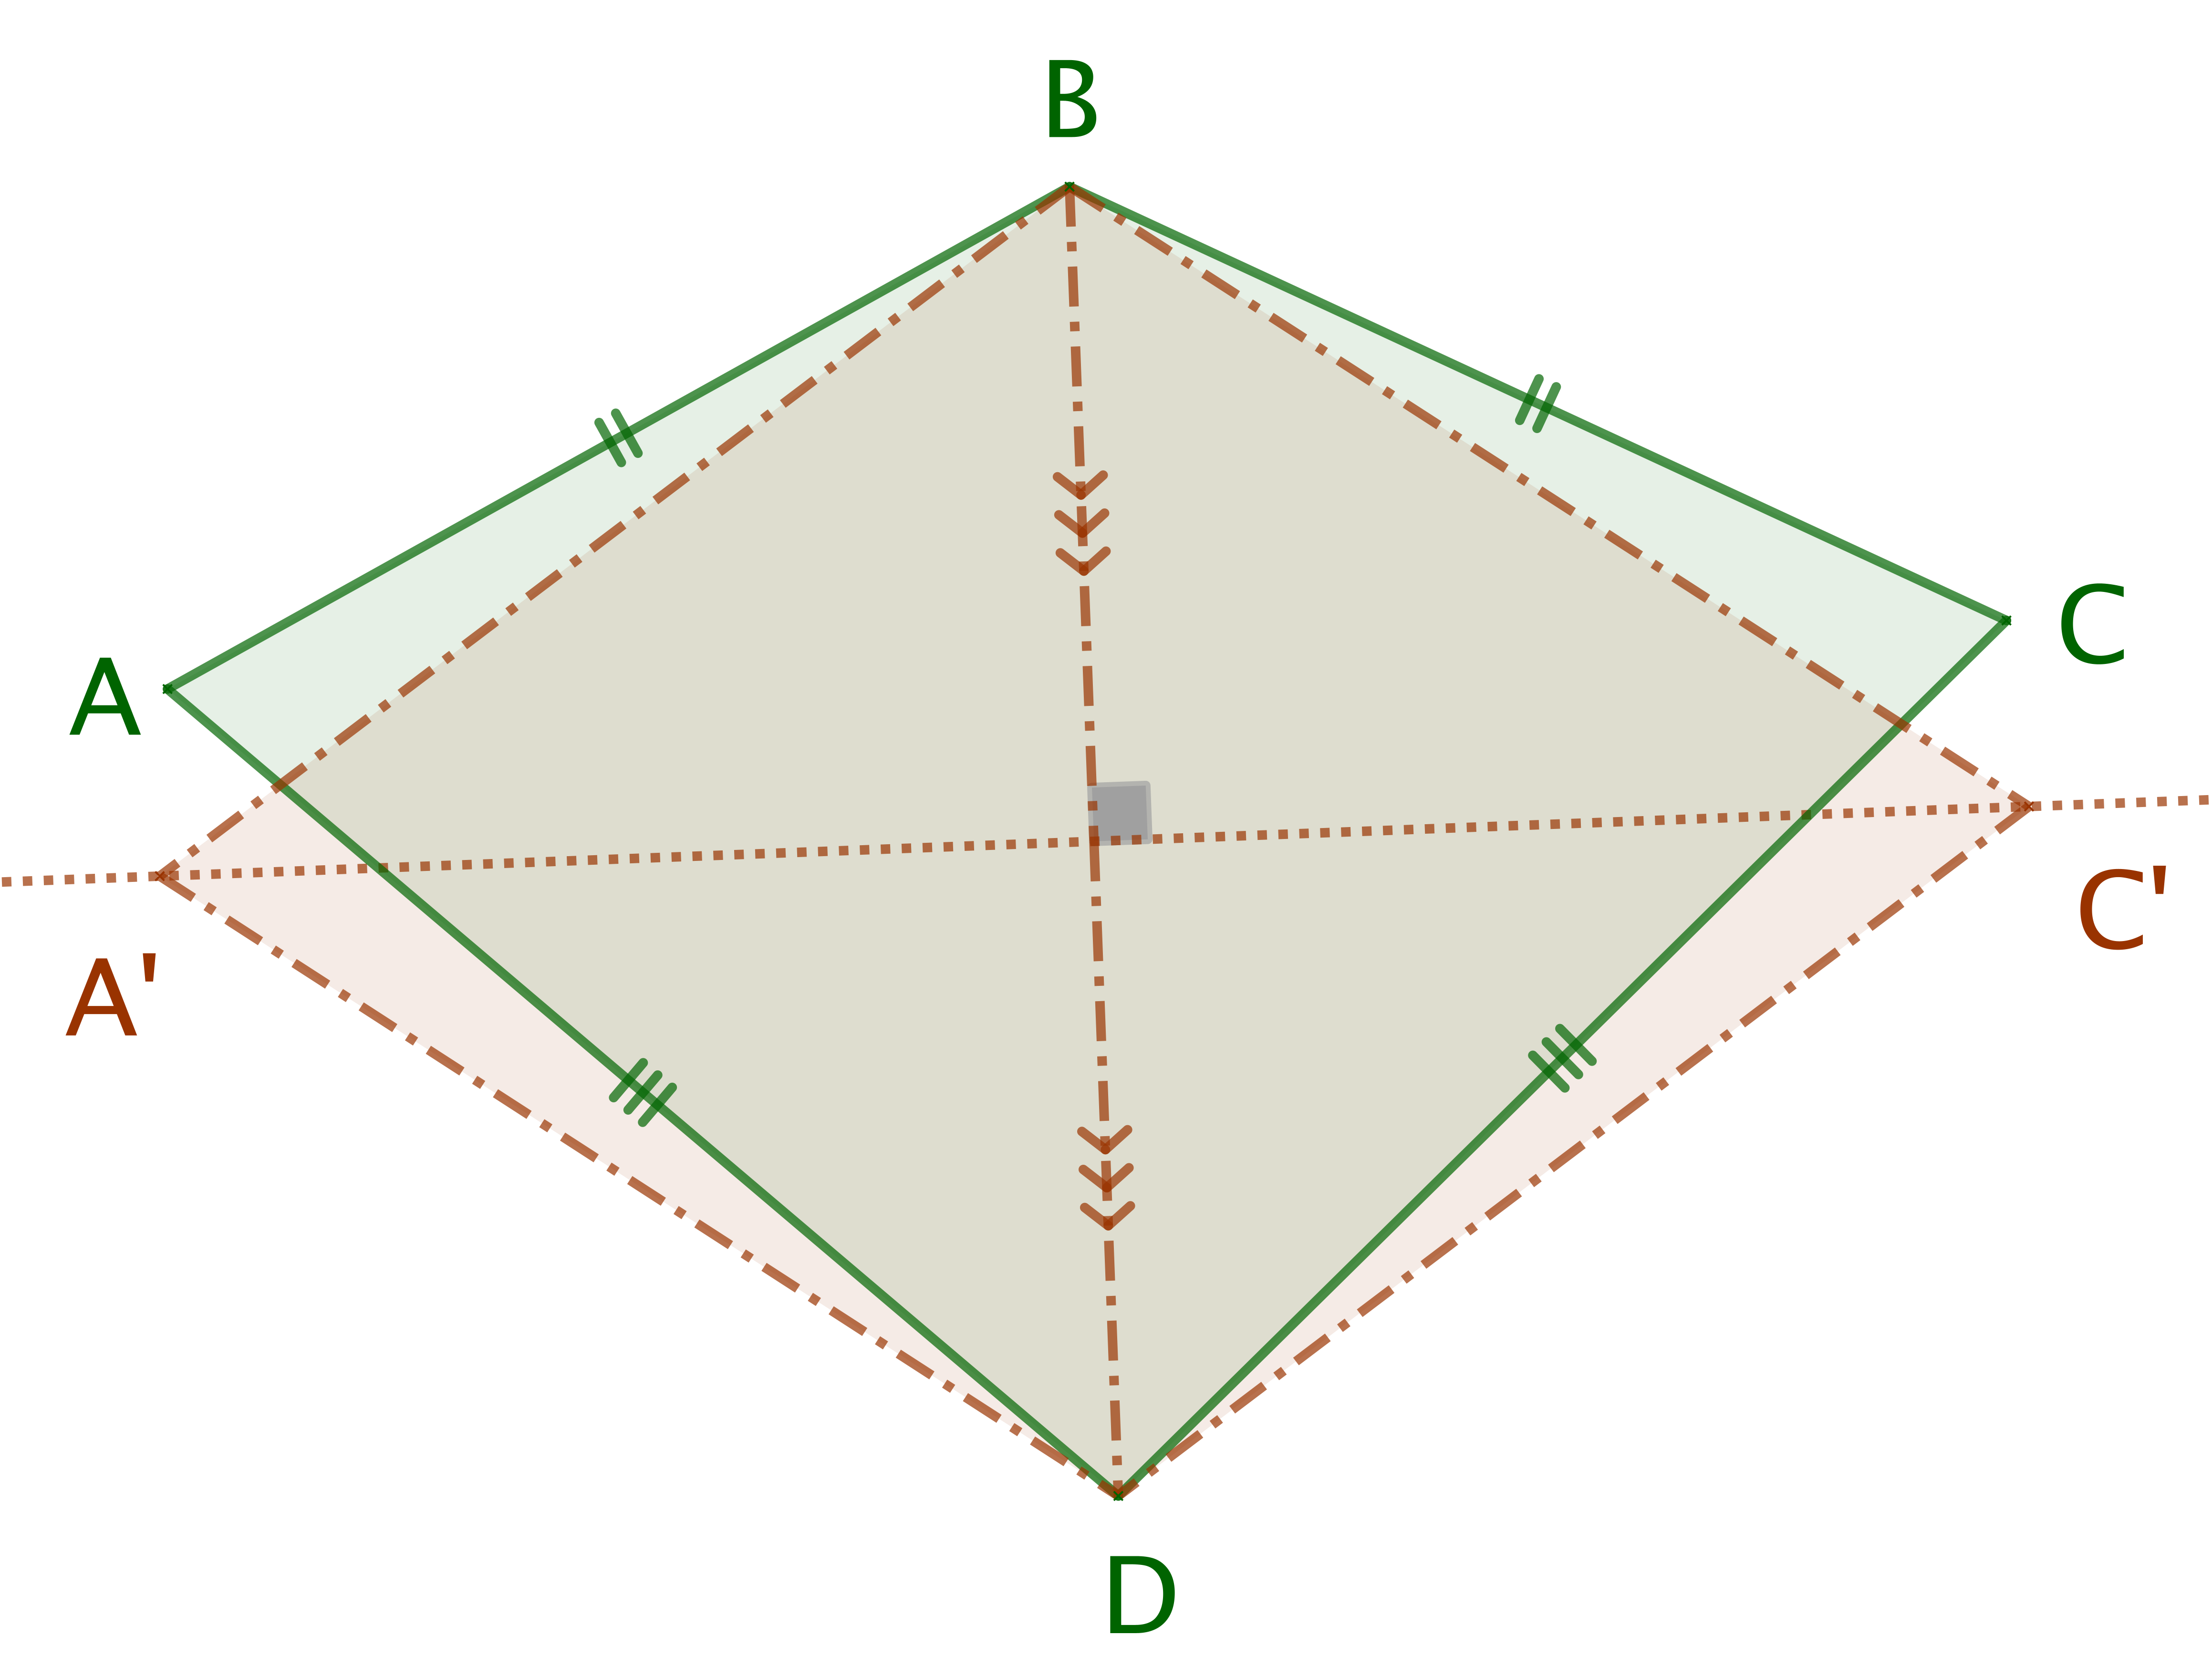
\includegraphics[scale=.4]{content/quadrilateral/quadrilateral-convex-isopaire.png}
	\end{center}
	
	
	Pour conclure, il suffit d'appliquer le fait \ref{iso-para}, puisque tout losange est un parallélogramme. Que la géométrie est belle!
\end{proof}


%
%
%% ------------- %
%
%
%\section{Les polygones}
%
%\subsection{Où allons-nous?}
%Le passage aux polygones à $n$ côtés, pour $n \geq 5$, va mêler analyse et géométrie: nous utiliserons les notions de compacité, de continuité, de convexité \focus{élargie} et de déterminant.


\begin{tcolorbox}
    \itshape\small
    L'approche proposée n'est pas originale dans sa globalité: voir, par exemple, "Isopérimètres en toute simplicité" de Lion Georges dans Bulletin de l'APMEP. N° 496., page 566-578.%
    \footnote{
        L'auteur du présent texte n'a eu connaissance du document de Lion Georges, qu'une fois son modeste travail fini.
    }
    Par contre, vous trouverez ici une approche la plus simple possible, et sans trous logiques.
\end{tcolorbox}

%
%
%\subsection{Quelques définitions}
%Pour l'existence d'au moins une solution, via des outils d'analyse, nous allons devoir sortir de l'ensemble des polygones en travaillant avec des objets plus souples, à savoir les \ncycles\ que nous définissons tout de suite.


% ----------------------- %


\begin{defi}
	Pour $n \in \NN_{\geq3}$, un \og \emph{\ncycle} \fg\ désigne une liste ordonnée de $n$ points du plan, les répétitions étant possibles.
	Nous noterons $A_1 A_2 \cdots A_n$ un \ncycle, et appellerons \og \emph{sommets}\fg\ du \ncycle\ les points $A_i$ pour $i \in \ZintervalC{1}{n}$.
\end{defi}


\begin{defi}
    Pour tout \ncycle\ $A_1 A_2 \cdots A_n$, on définit $\big( A^{\,\prime}_i \big)_{i \in \ZZ}$ comme étant $n$-périodique, et vérifiant $A^{\,\prime}_{i} = A_i$ sur $\ZintervalC{1}{n}$.
\end{defi}


\begin{defi}
	Les \og \emph{côtés} \fg\ d'un \ncycle\ $\setproba{L} = A_1 A_2 \cdots A_n$ sont les segments
	$[A^{\,\prime}_i A^{\,\prime}_{i+1}]$ pour $i \in \ZintervalC{1}{n}$,
	et
	la \og \emph{longueur} \fg\ de $\setproba{L}$ est définie par $\cyclelen{\setproba{L}} = \dsum_{i=1}^{n} A^{\,\prime}_i A^{\,\prime}_{i+1}$.
\end{defi}


\begin{defi}
	Un \ncycle\ $\setproba{L} = A_1 A_2 \cdots A_n$ est dit \og \emph{convexe} \fg\ si, pour chaque côté $[A^{\,\prime}_i A^{\,\prime}_{i+1}]$, tous les sommets de $\setproba{L}$ sont dans un même demi-plan fermé délimité par la droite $(A^{\,\prime}_i A^{\,\prime}_{i+1})$ (un sommet peut donc être sur cette droite).
\end{defi}


\begin{defi}
	Un \ncycle\ est \og \emph{dégénéré} \fg\ s'il a, au moins, trois sommets consécutifs alignés.
\end{defi}


\begin{center}
	\small\itshape\centering
	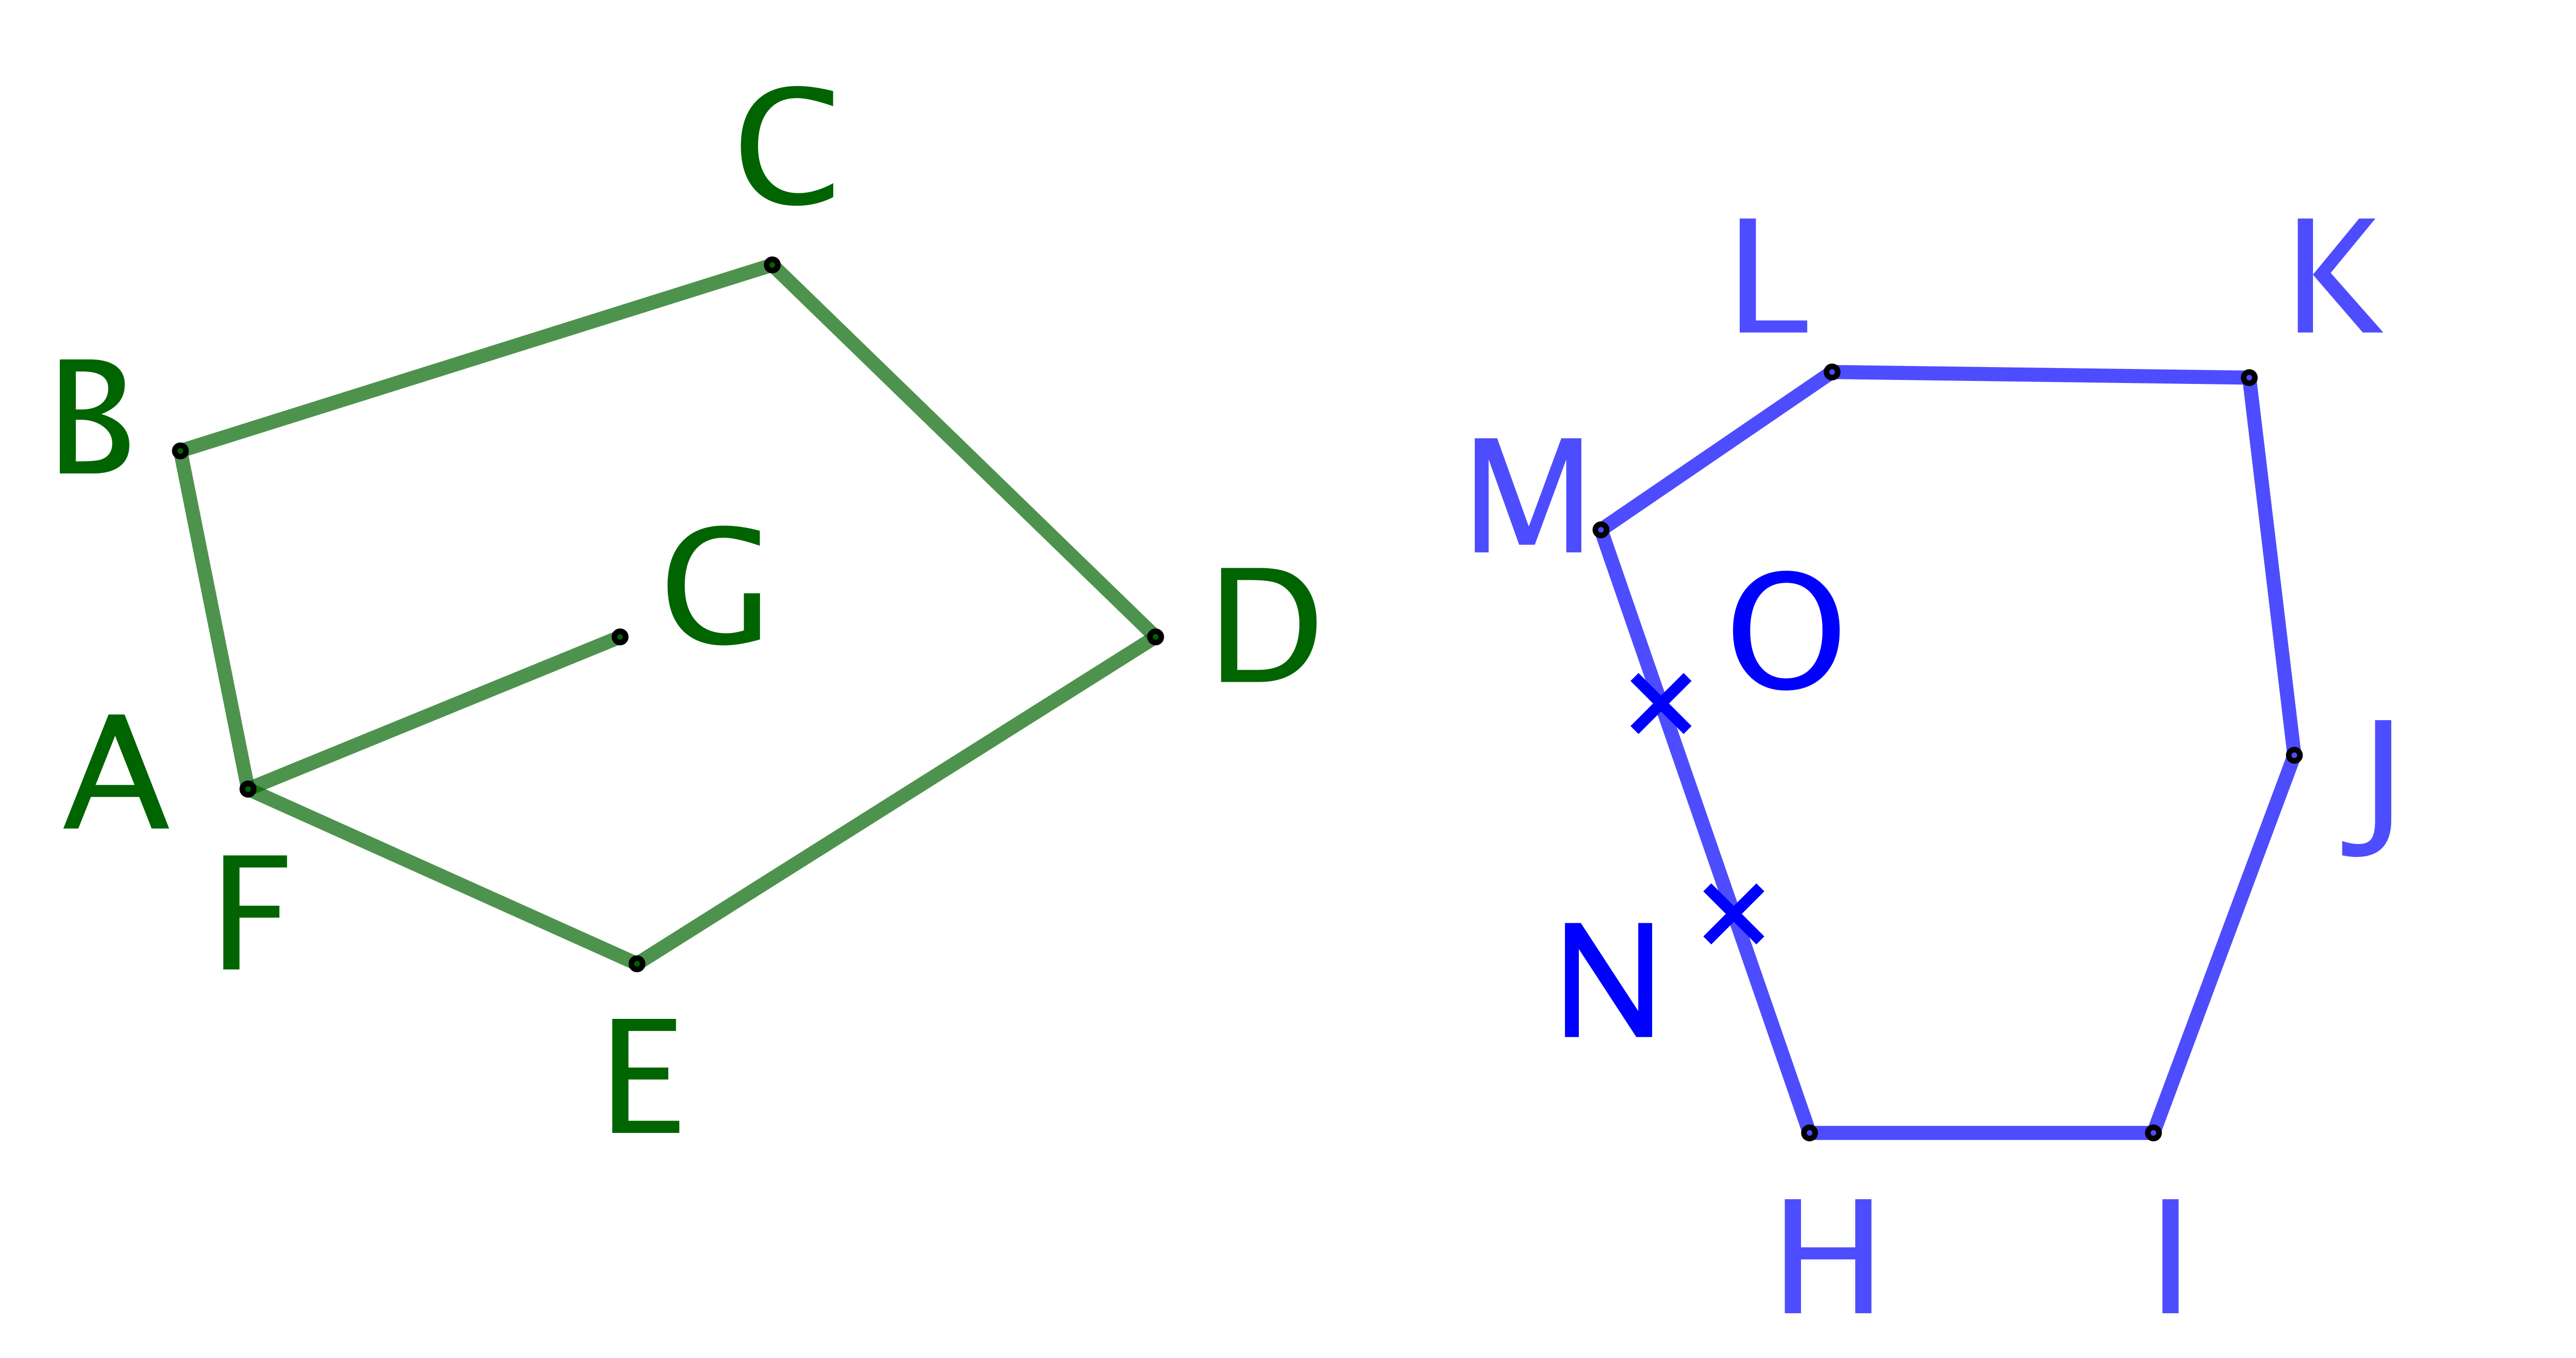
\includegraphics[scale=.35]{content/polygon/def/degenerated-ncycles.png}
	
	\smallskip
	$ABCDEFG$ est un \ncycle\ ni dégénéré, ni convexe, et qui n'est pas un \ngone.
	
	\smallskip
	$HIJKLMNO$ est un \ncycle\ dégénéré et convexe.
\end{center}


% ----------------------- %


\newpage

\begin{defi}
	Un \og \emph{\ngone} \fg\ $\setproba{P}$ est un \ncycle\ vérifiant les conditions suivantes qui impliquent $n \geq 3$, et que les sommets sont distincts deux à deux.
	%
	\begin{itemize}
		\item Les côtés de $\setproba{P}$ contienne tous exactement deux sommets.

		\item Des côtés non contigus de $\setproba{P}$ ne sont jamais sécants.
	\end{itemize}


	Si certains côtés non contigus sont sécants en un point, mais tous les sommets distincts deux à deux, nous parlerons de \og \emph{\ngone\ croisé} \fg.%
	\footnote{
		Bien retenir que, par définition, un \ngone\ n'est jamais croisé.
		Dès lors, la longueur d'un \ngone\ correspond à son périmètre.
	}
\end{defi}


\begin{defi}
	Un \ngone, croisé ou non, est dit \og \emph{équilatéral} \fg\ si tous ses côtés sont de même mesure.
\end{defi}


\begin{defi}
	Un \ngone, croisé ou non, est dit \og \emph{équiangle} \fg\ si tous ses angles au sommet sont de même mesure.
\end{defi}


\begin{defi}
	Un \ngone, croisé ou non, est dit \og \emph{régulier} \fg\ s'il est à la fois équiangle et équilatéral.
\end{defi}


\begin{remark}
	Un losange non carré est un \nequi\ convexe non régulier, et un rectangle non carré est un \niso\ convexe non régulier.
\end{remark}


\begin{remark}
	Il existe des \nregs\ et croisés.


    \vspace{-1.5em}
    
    \begin{multicols}{2}
    	\small\itshape\centering
    	
	    \null\vfill

	    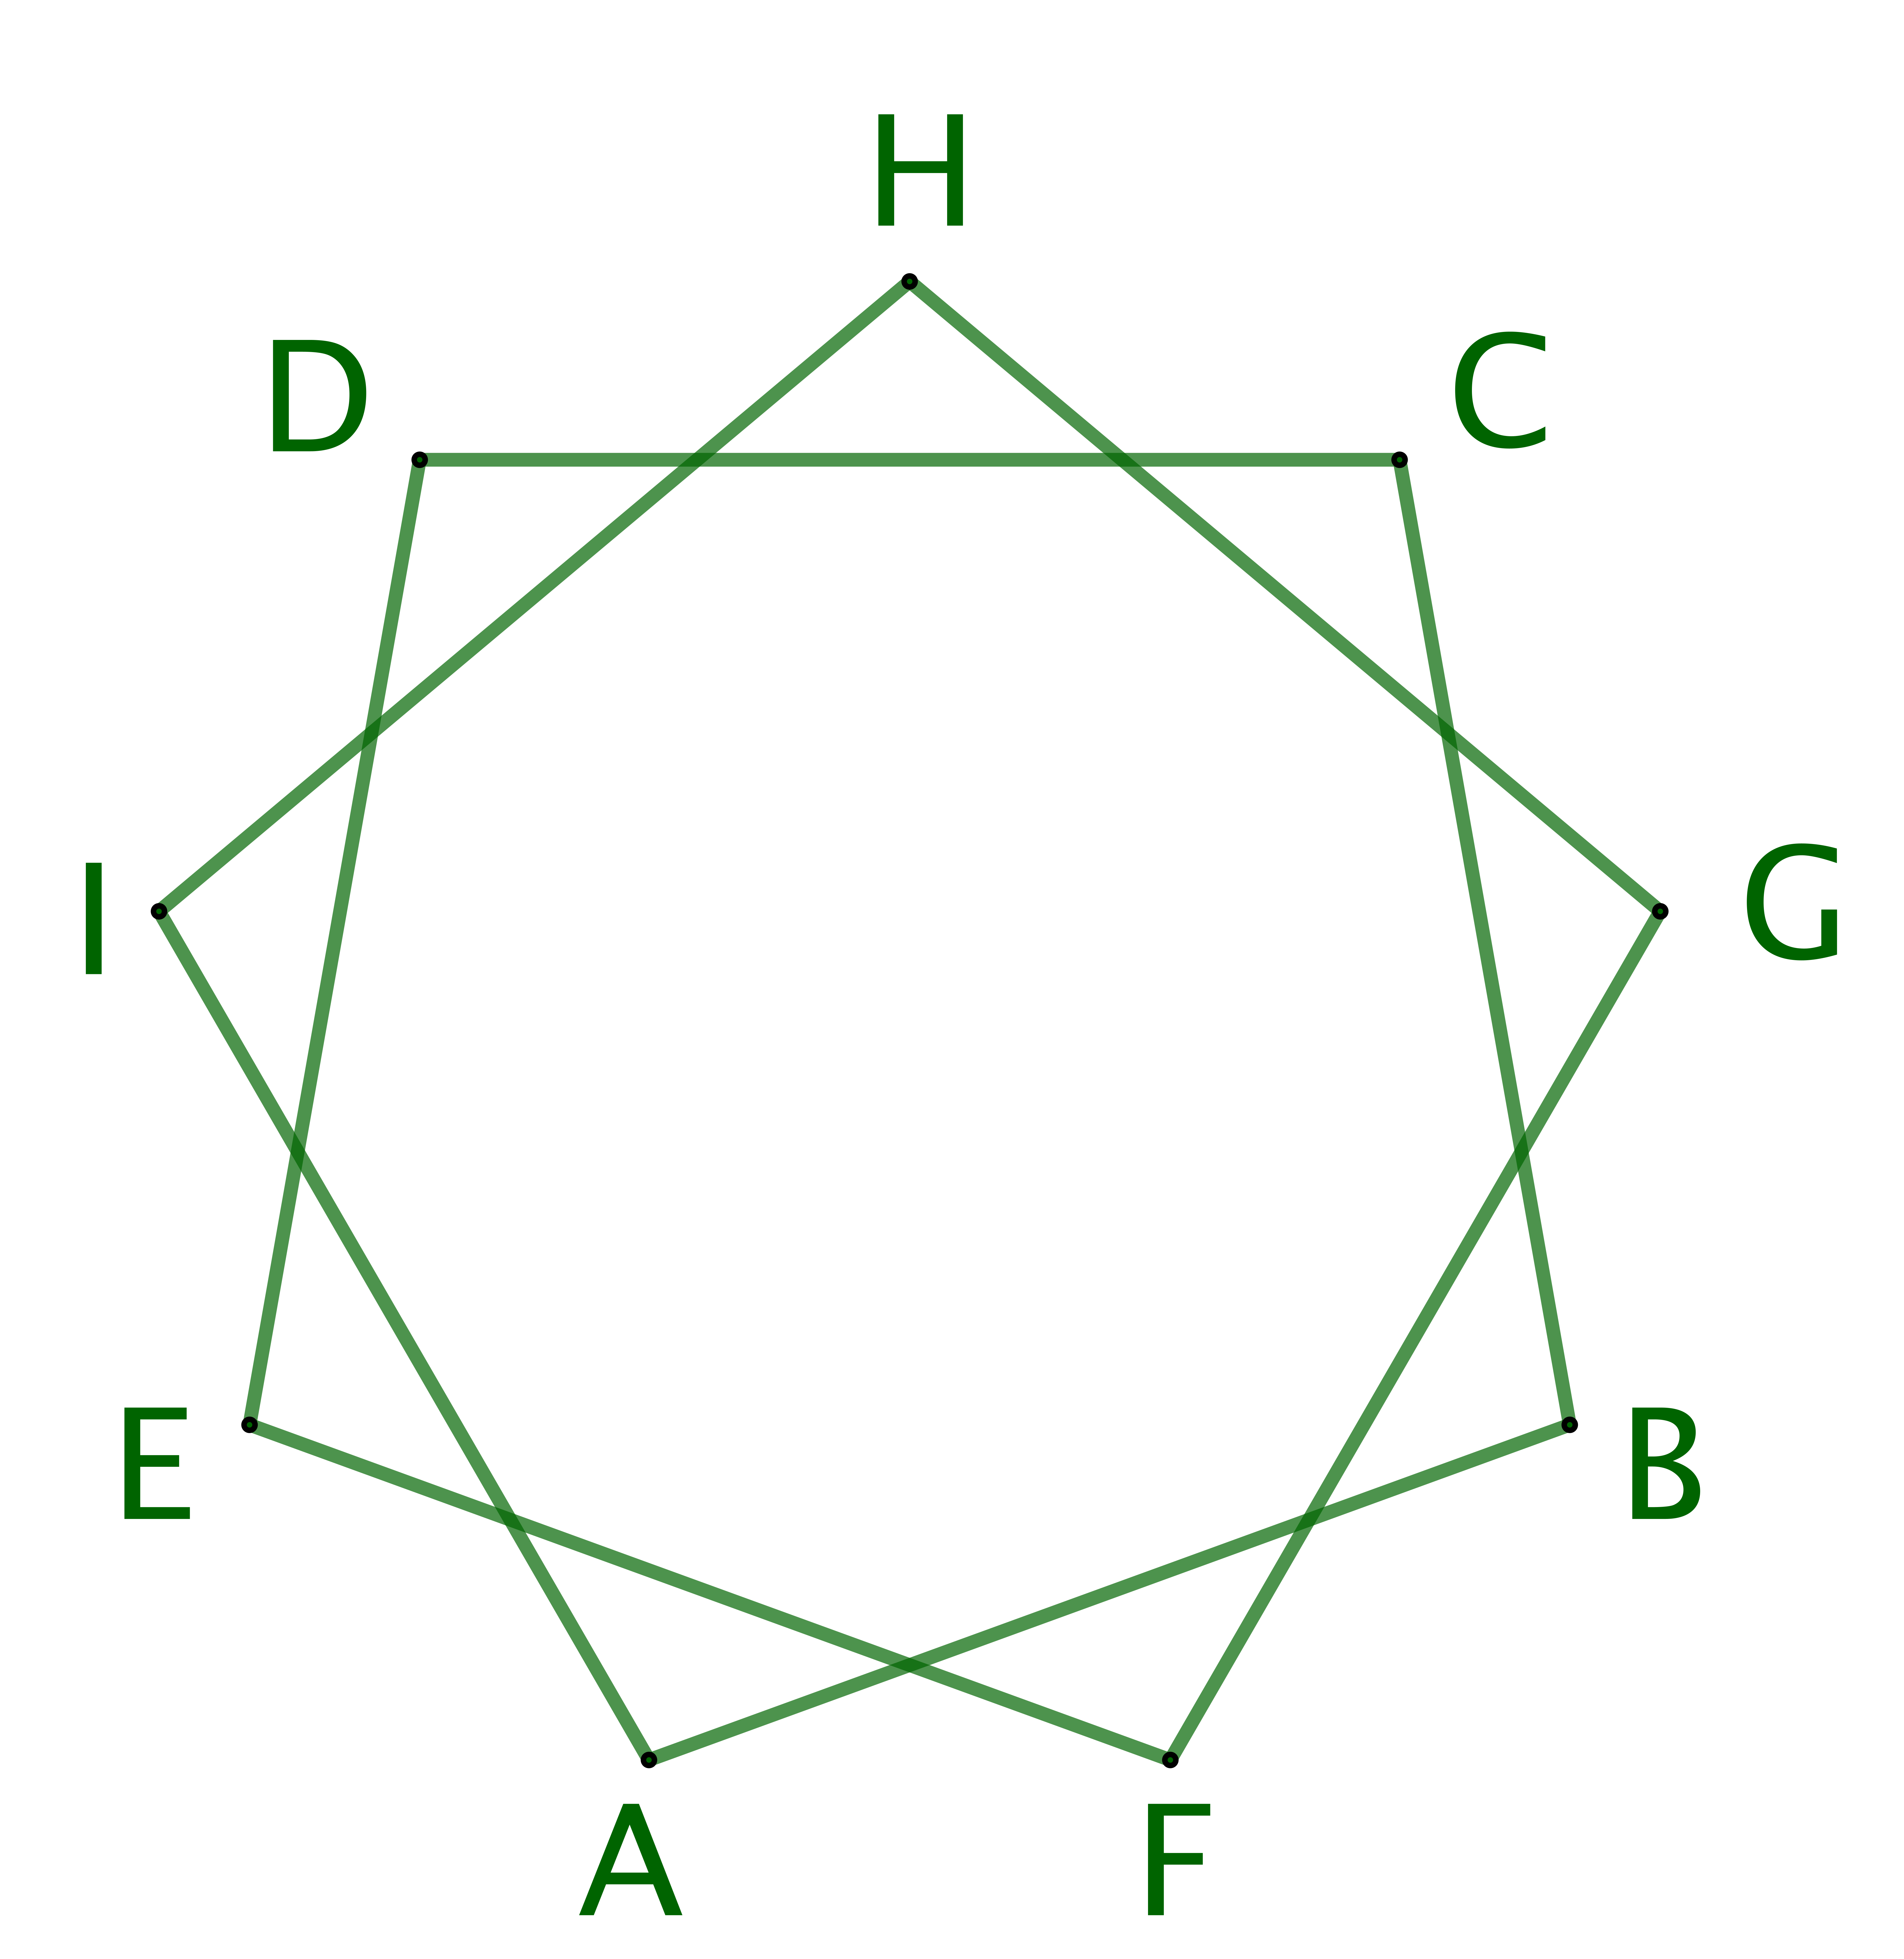
\includegraphics[scale=.175]{content/polygon/def/9-iso-non-conv.png}
    
        \smallskip
        Un ennéagone régulier croisé dit étoilé.%
	    \footnote{
	        La construction se fait via $AFBGCHDIE$ qui est un \xreg{9} convexe. Elle se généralise à tout \nreg\ tel que $n$ soit impair.
	    }

%	    \vfill\null

    	\columnbreak
	
	    \null\vfill
	    
	    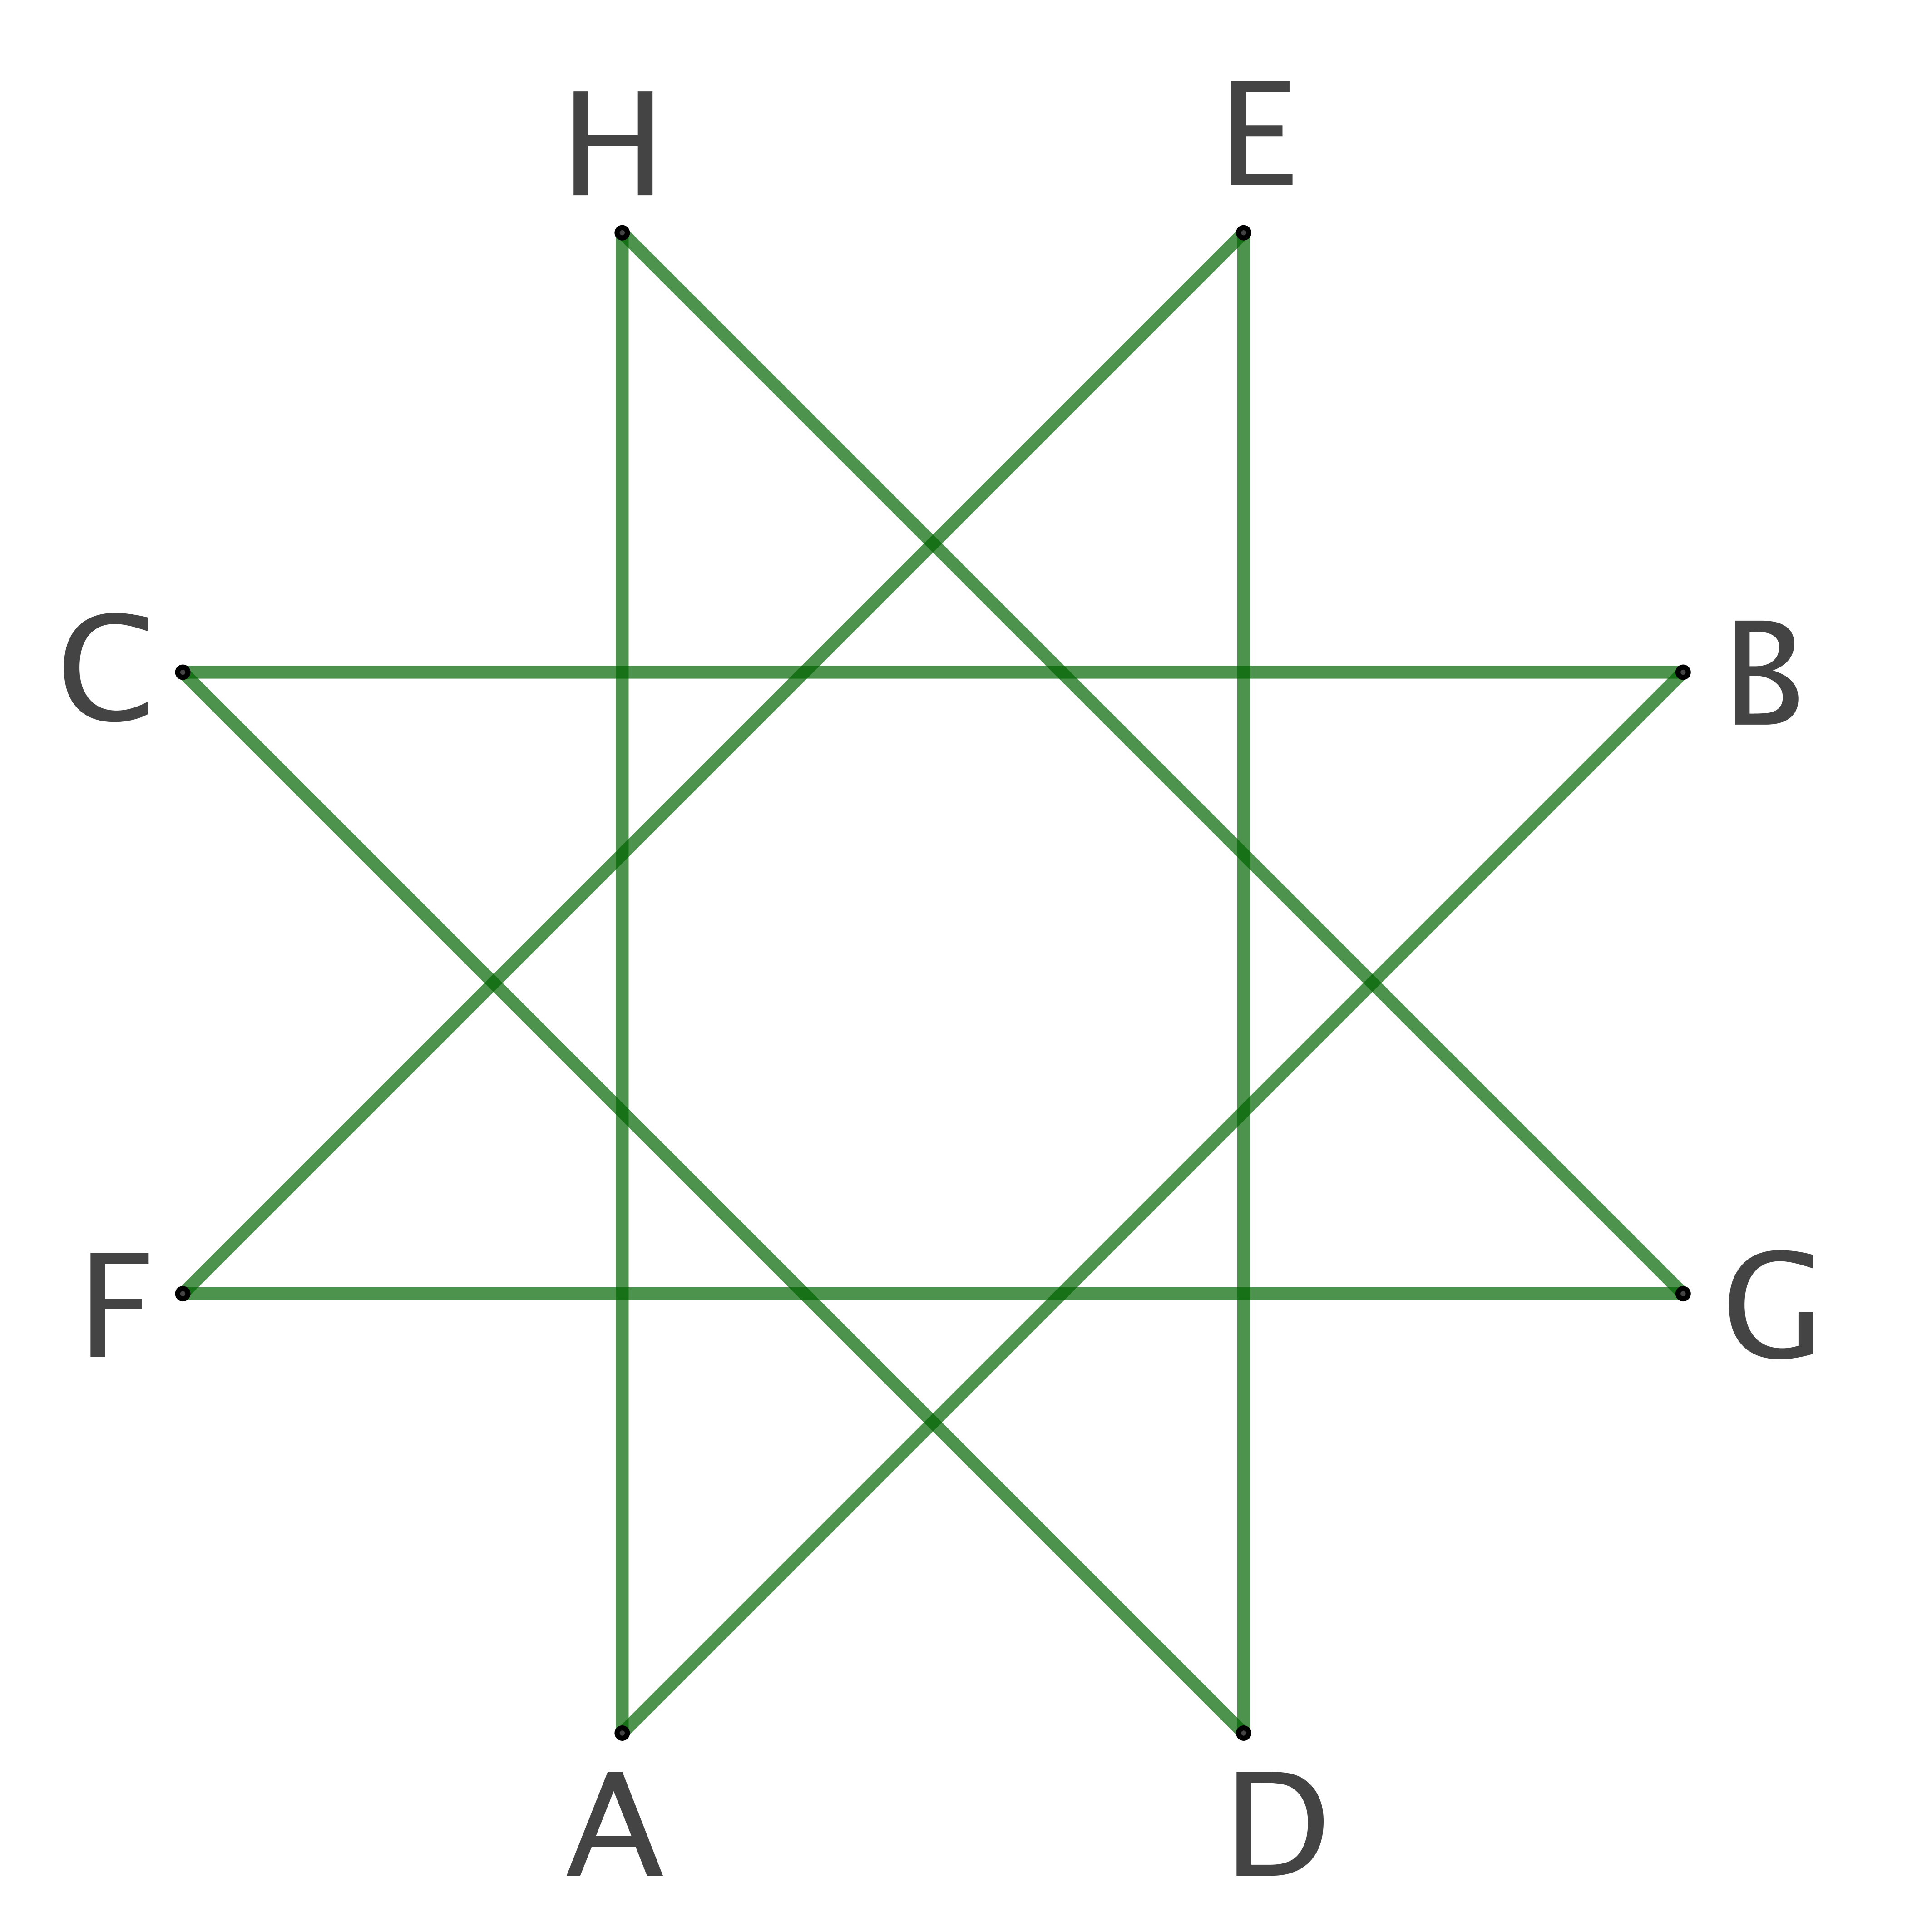
\includegraphics[scale=.3]{content/polygon/def/8-iso-non-conv.png}
    
        \smallskip
        Un octogone régulier croisé dit étoilé.%
	    \footnote{
	        La construction se fait via le \xreg{8} convexe intérieur. Elle se généralise à tout \nreg\ tel que $n$ soit pair.
	    }

%	    \vfill\null
    \end{multicols}
\end{remark}

%
%
%\subsection{Aire algébrique d'un \ncycle}
%Pour prouver l'existence d'un \ngone\ solution du problème d'isopérimétrie polygonale, il faut un moyen \og continu \fg\ de calculer une aire polygonale. L'outil que nous allons utiliser est l'aire algébrique qui est définie pour tout \ncycle\ $\setproba{L} = A_1 A_2 \cdots A_n$ par $\frac12 \dsum_{i=1}^{n} \det \big( \vect{\Omega A^{\,\prime}_i} , \vect{\Omega A^{\,\prime}_{i+1}} \big)$ indépendamment du point $\Omega$.%
\footnote{
    Ce fait est démontré un peu plus bas.
}

Indiquons au passage qu'il faut être prudent avec cette notion comme le montre l'exemple suivant, obtenu avec \geogebra,%
\footnote{
	Quand \geogebra\ associe un nombre à un \ncycle\ $\setproba{L}$, il calcule la valeur absolue de son aire algébrique.
}
où le \ngone\ croisé proposé, construit via une spirale positive depuis le point $A$,%
\footnote{
	En calculant l'aire algébrique avec un point \og au centre \fg, les déterminants sont tous positifs.
} 
possède une aire algébrique positive supérieure à celle de l'enveloppe convexe du \ngone. Contre-intuitif, mais normal.


\begin{multicols}{2}
	\small\itshape\centering
	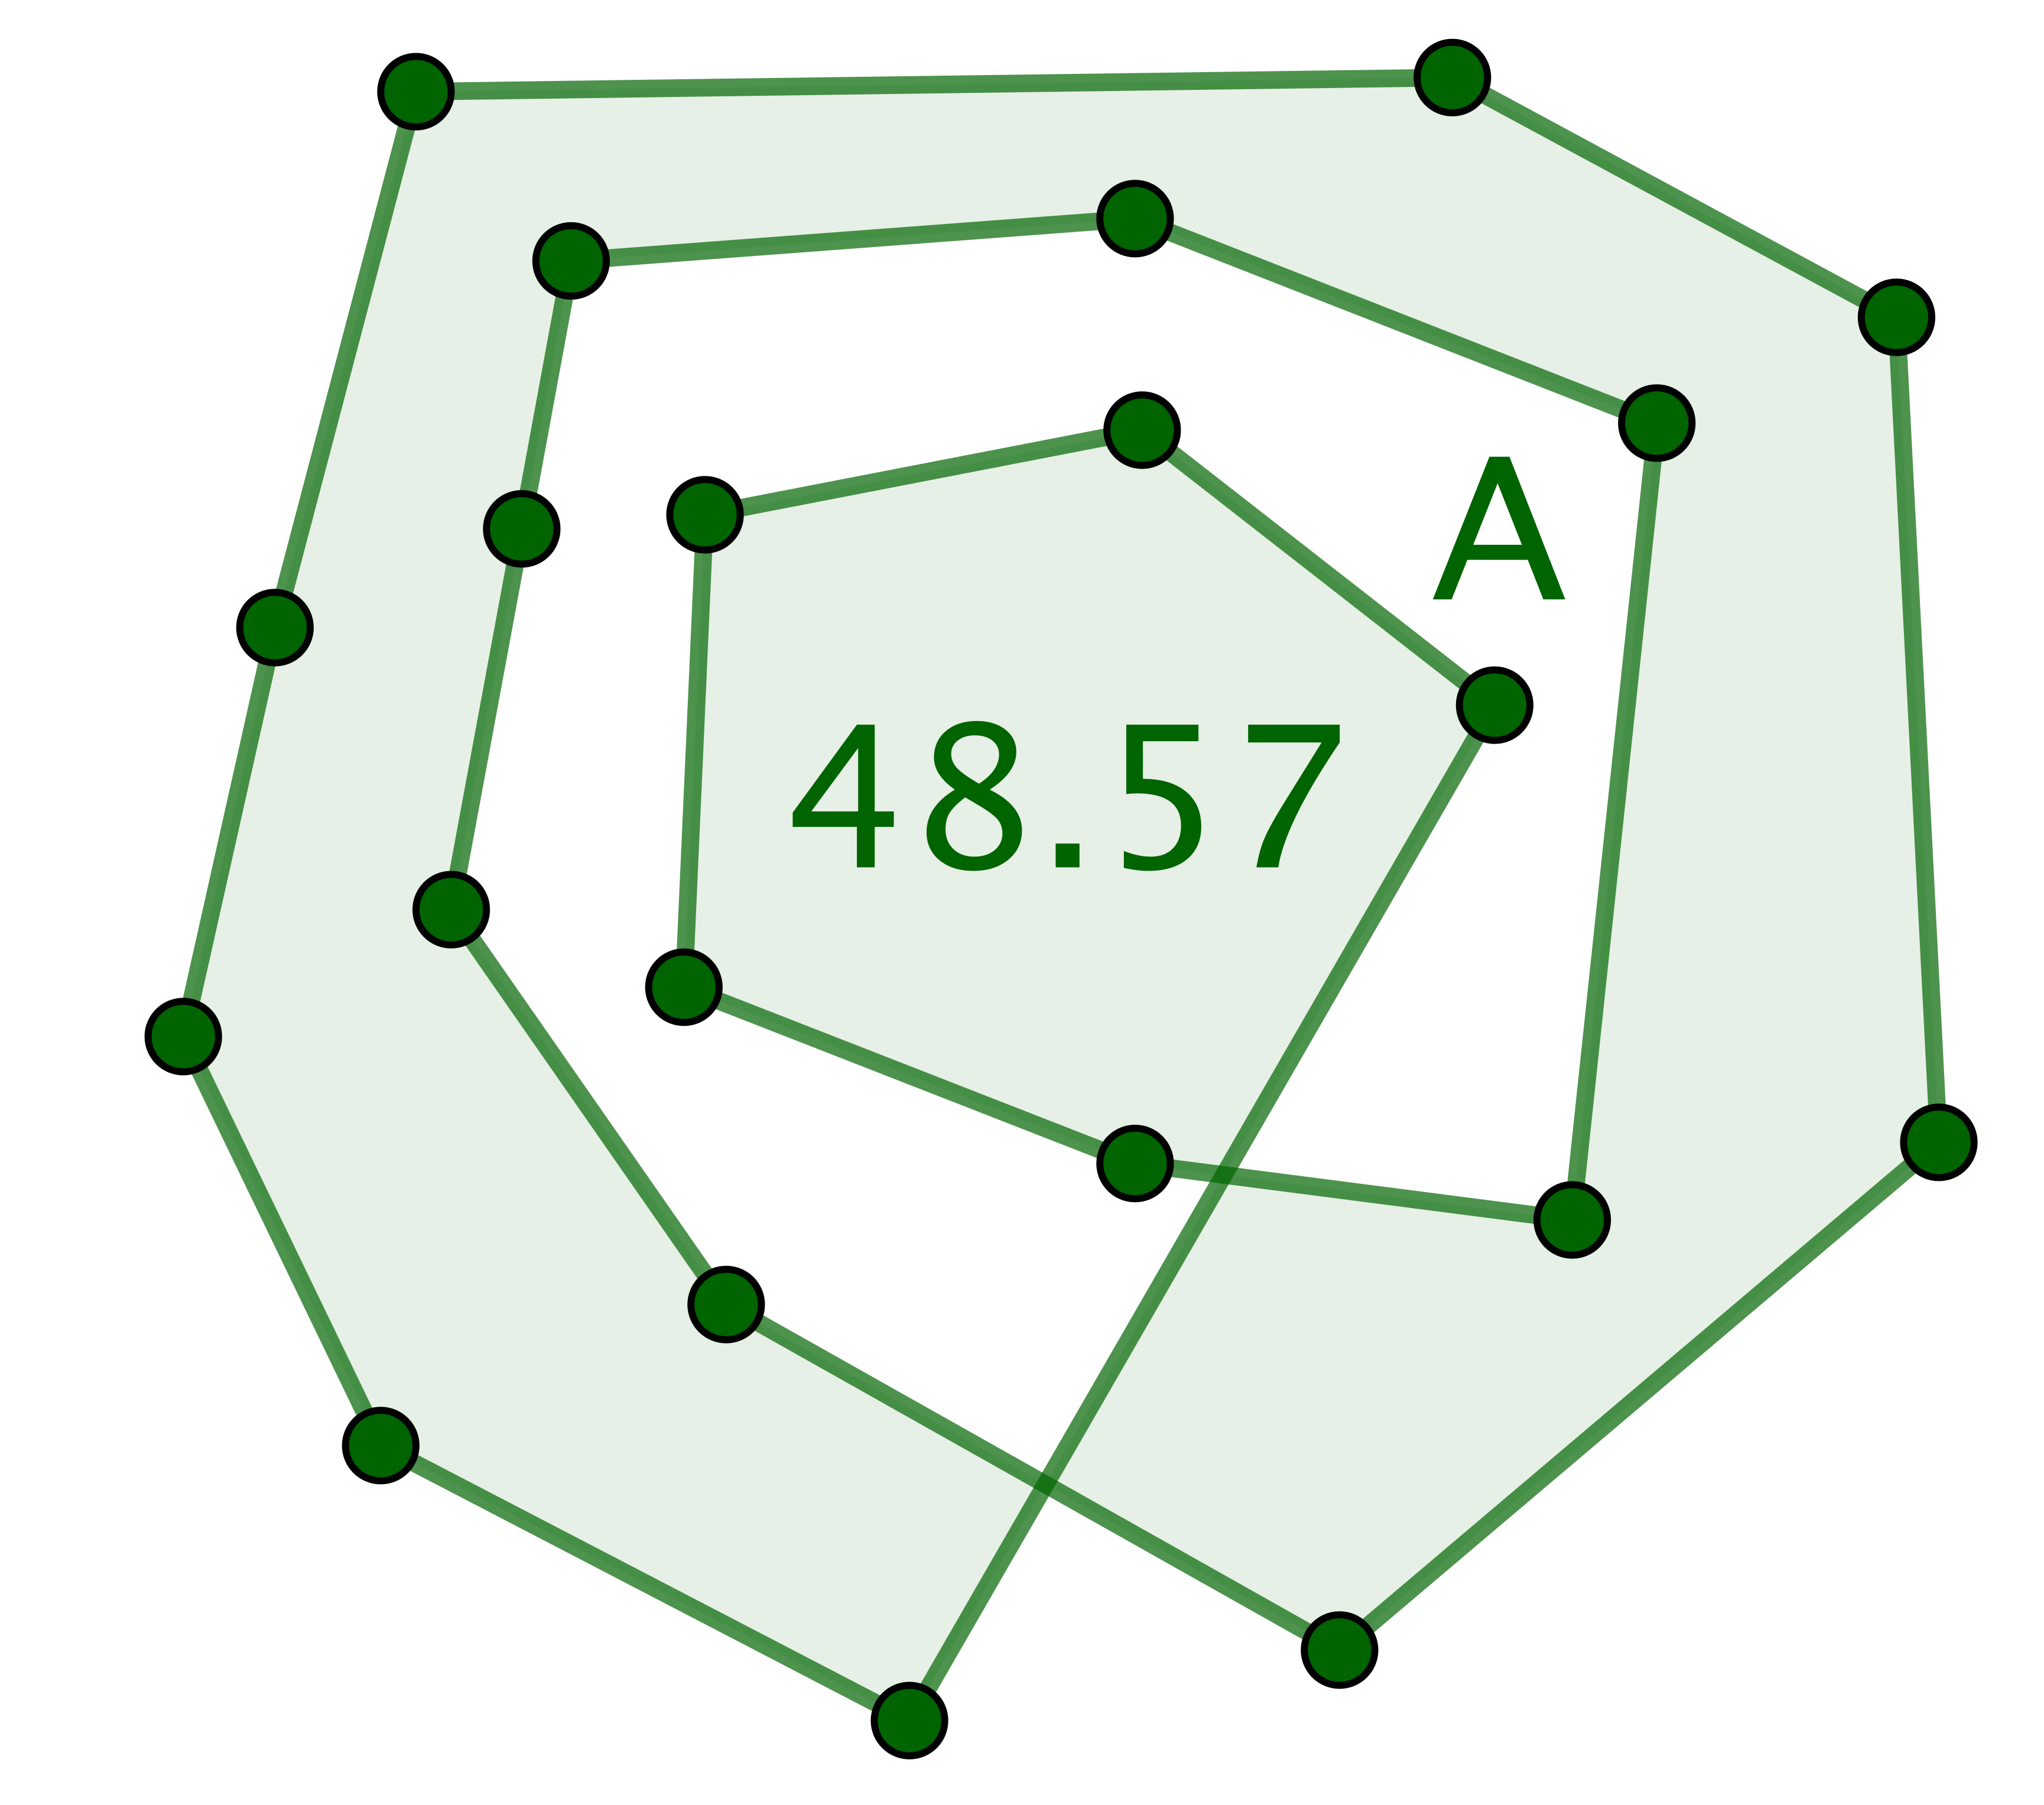
\includegraphics[scale=.3]{content/polygon/alg-area/alg-area-ncycle-not-opti-pb-1.png}

	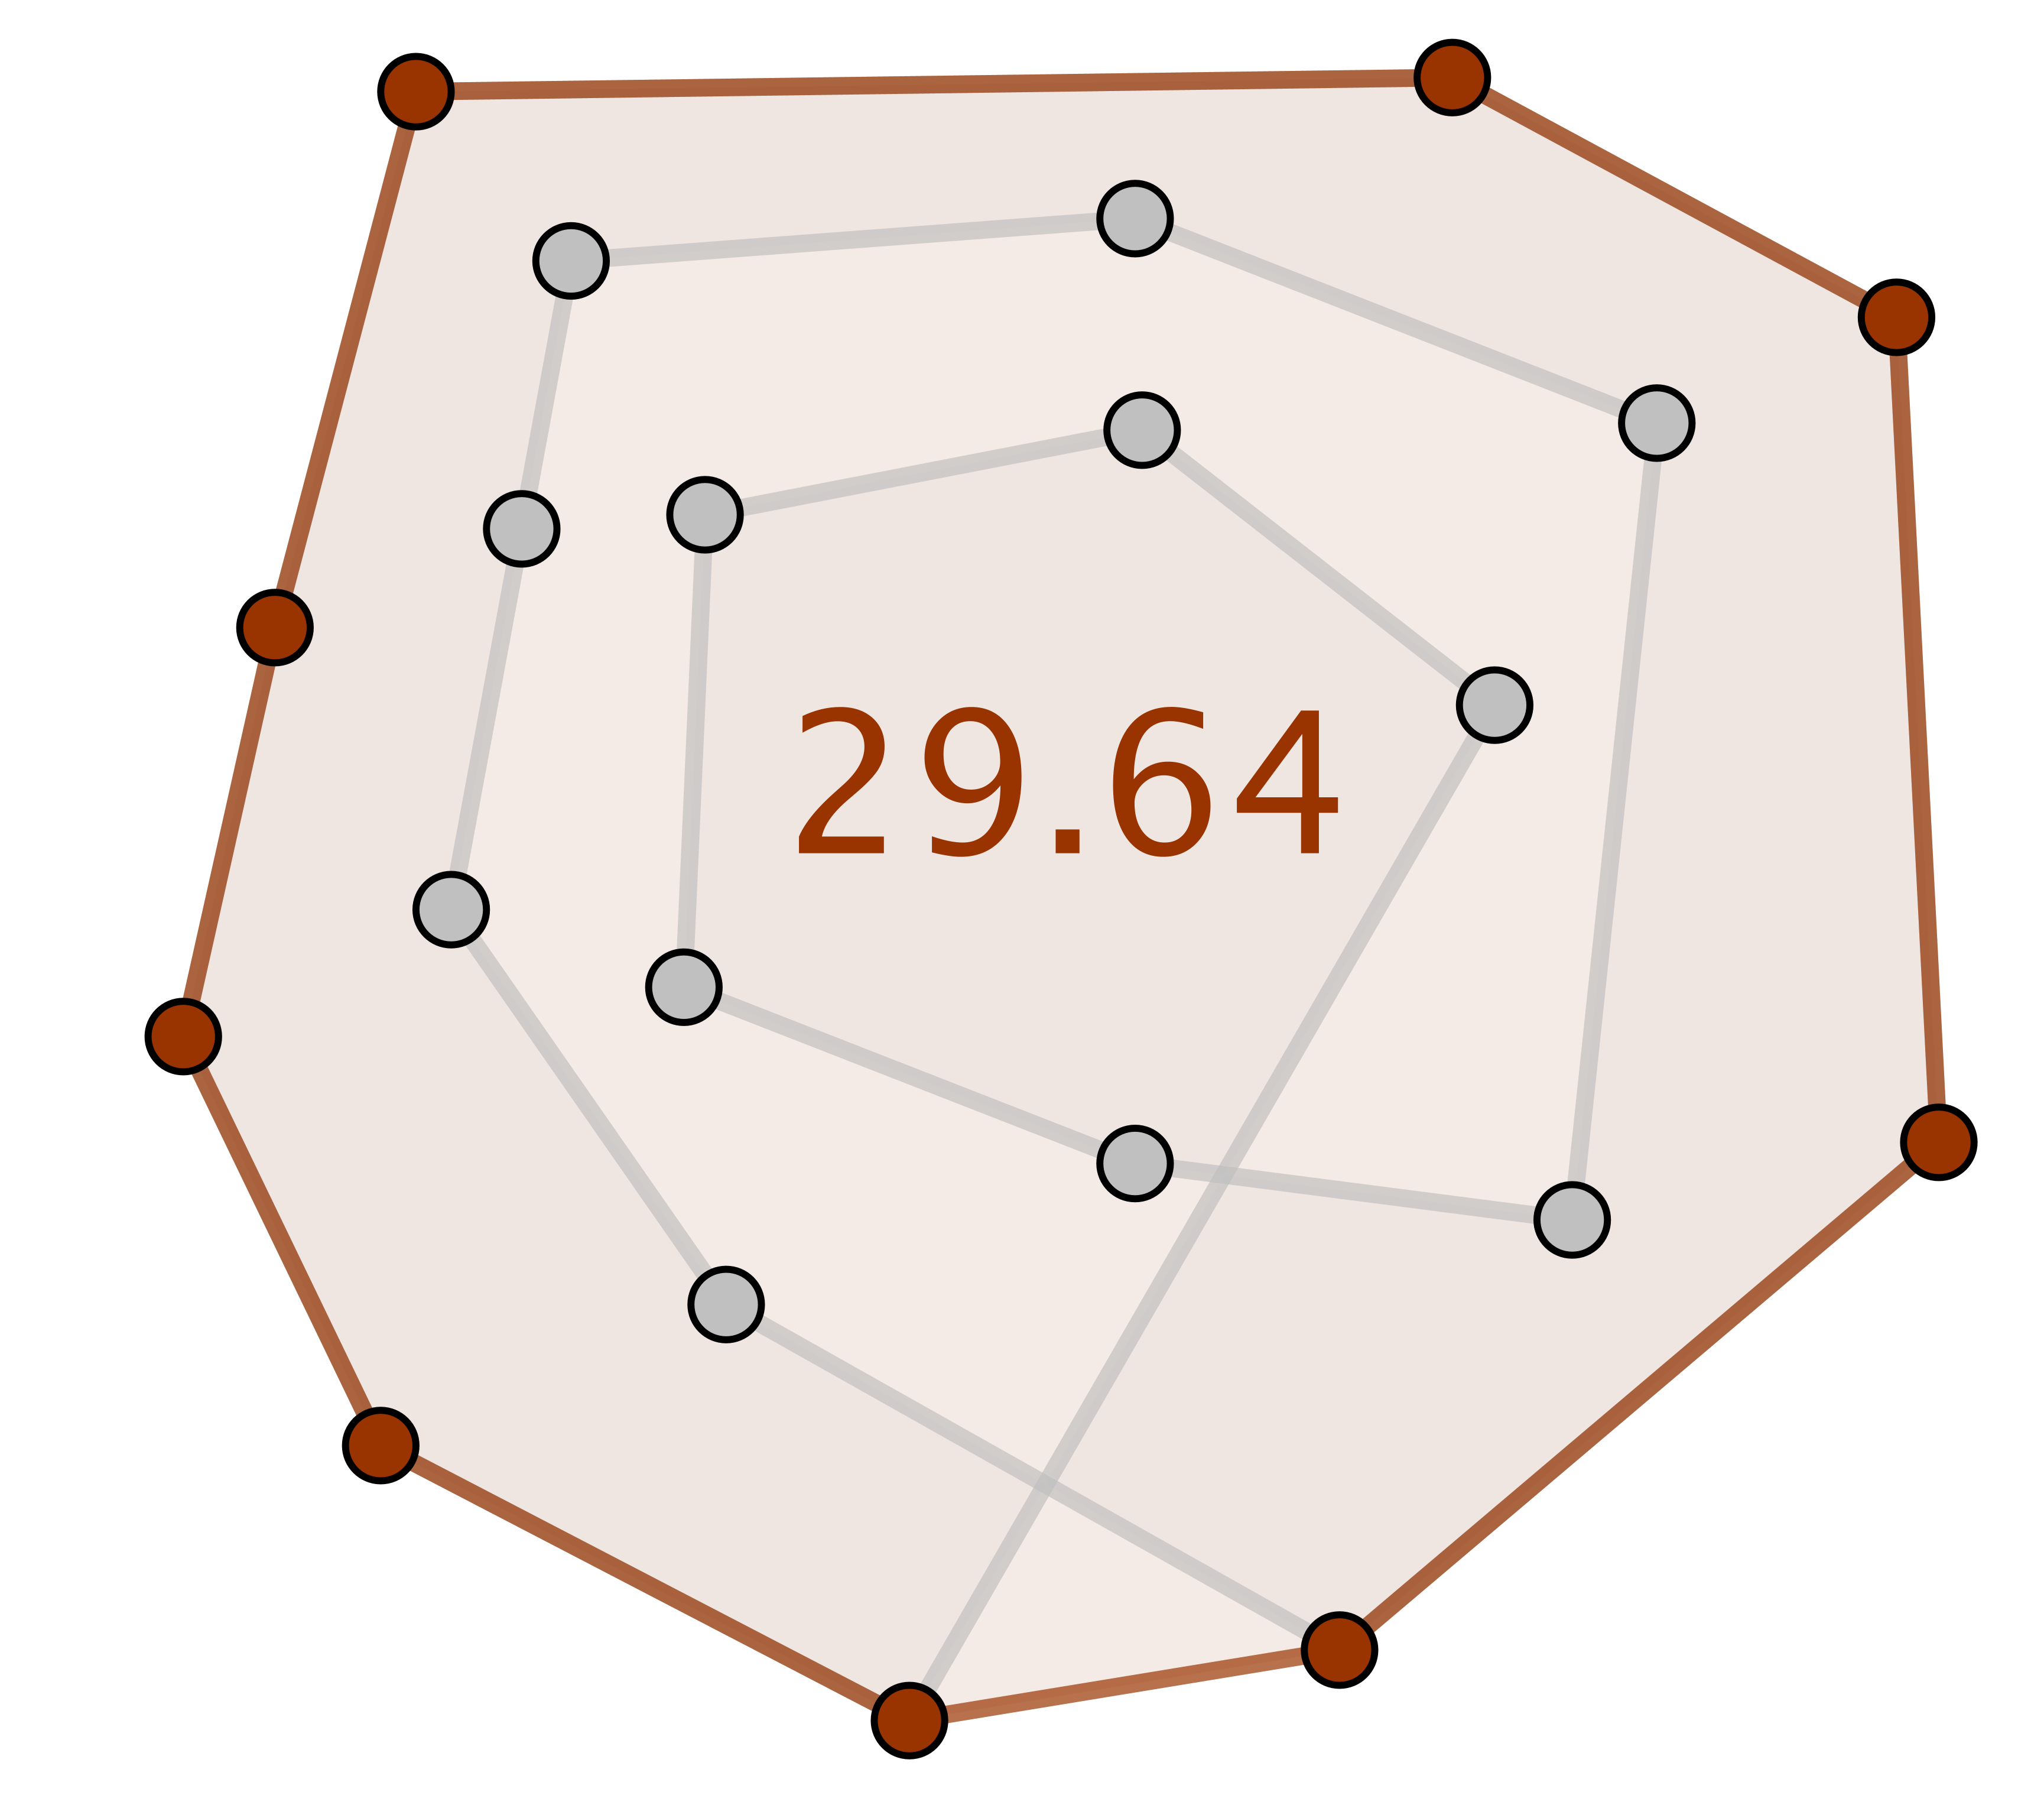
\includegraphics[scale=.3]{content/polygon/alg-area/alg-area-ncycle-not-opti-pb-2.png}
\end{multicols}


% ----------------------- %


Au commencement étaient les triangles... Il est connu que $ABC$ est d'aire $\frac12 \abs{ \det \big( \vect{AB} , \vect{AC} \big) }$ où $\frac12 \det \big( \vect{AB} , \vect{AC} \big)$ est appelé aire algébrique de $ABC$. Pour passer aux polygones, il \og suffit \fg\ d'utiliser des triangles comme dans l'exemple suivant.


\begin{multicols}{2}
	\small\itshape
    \begin{center}
		Calcul direct à la main.

		\smallskip

        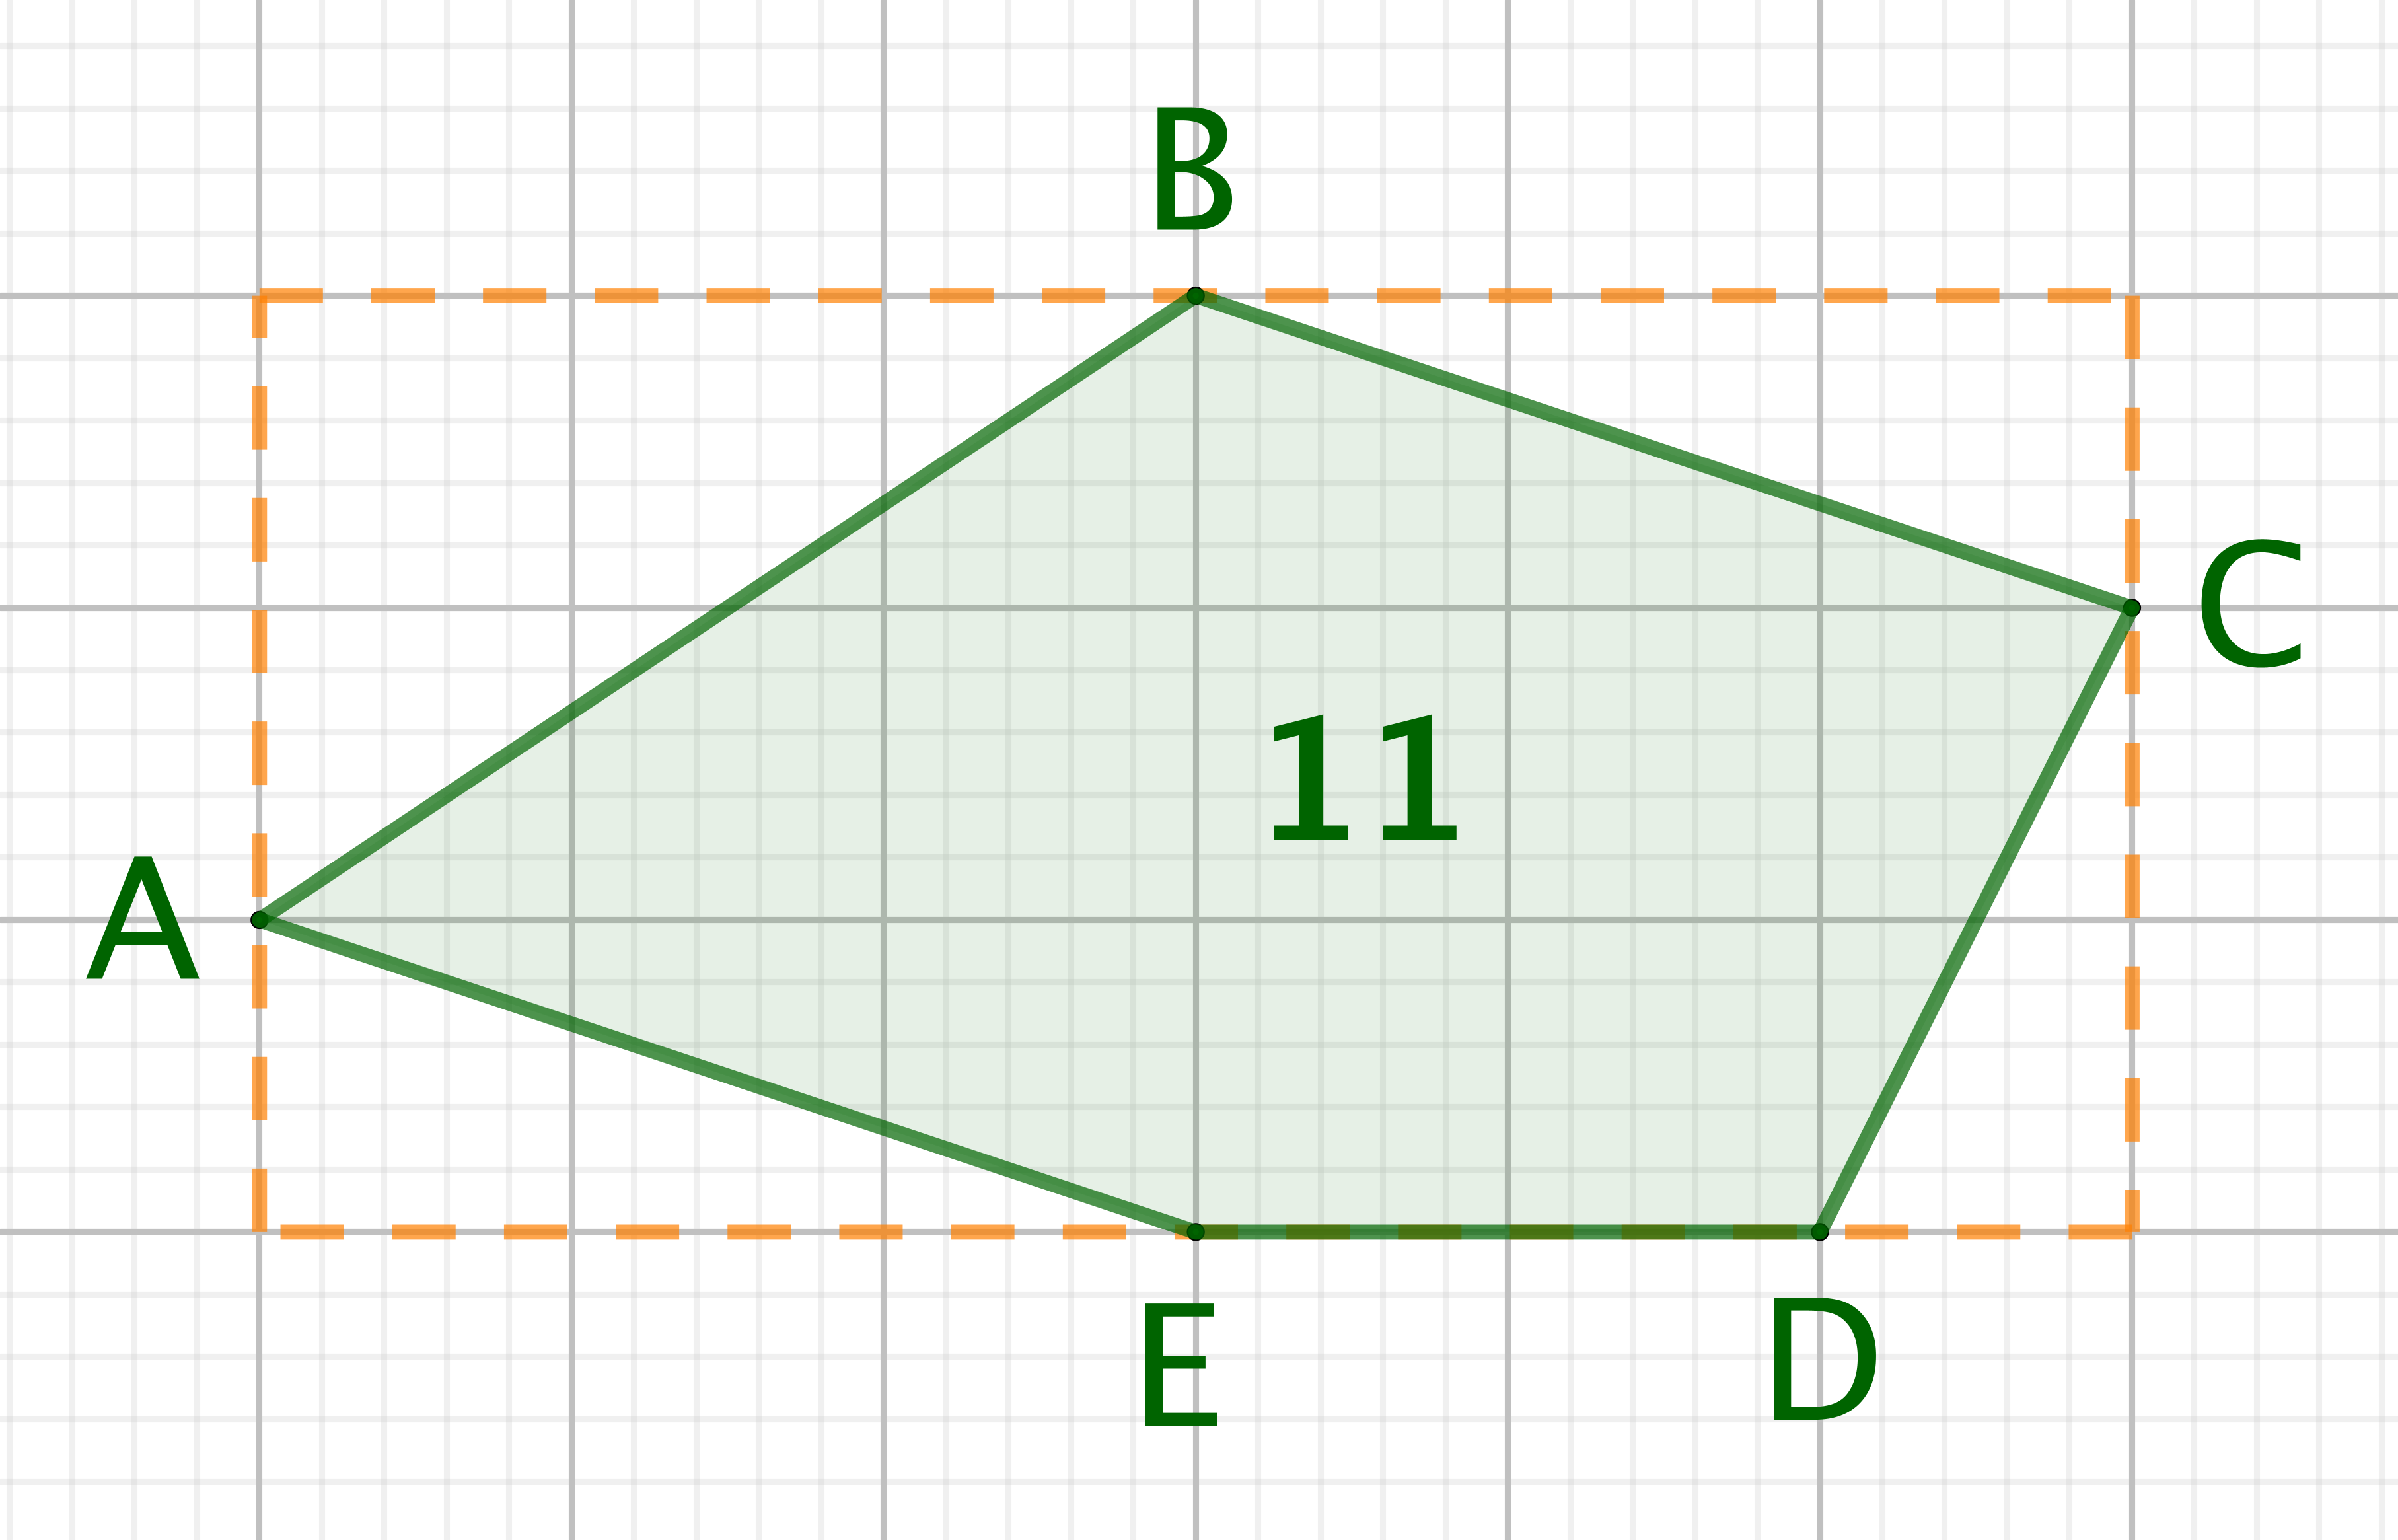
\includegraphics[scale=.35]{content/polygon/alg-area/convex-1.png}

       	\smallskip

		$11 = 3 \cdot 6 - \dfrac{3 \cdot 1 + 3 \cdot 2 + 3 \cdot 1 + 1 \cdot 2}{2} \vphantom{\dfrac{2^M}2}$
    \end{center}

	\columnbreak

    \begin{center}
		Via le déterminant.

		\smallskip

        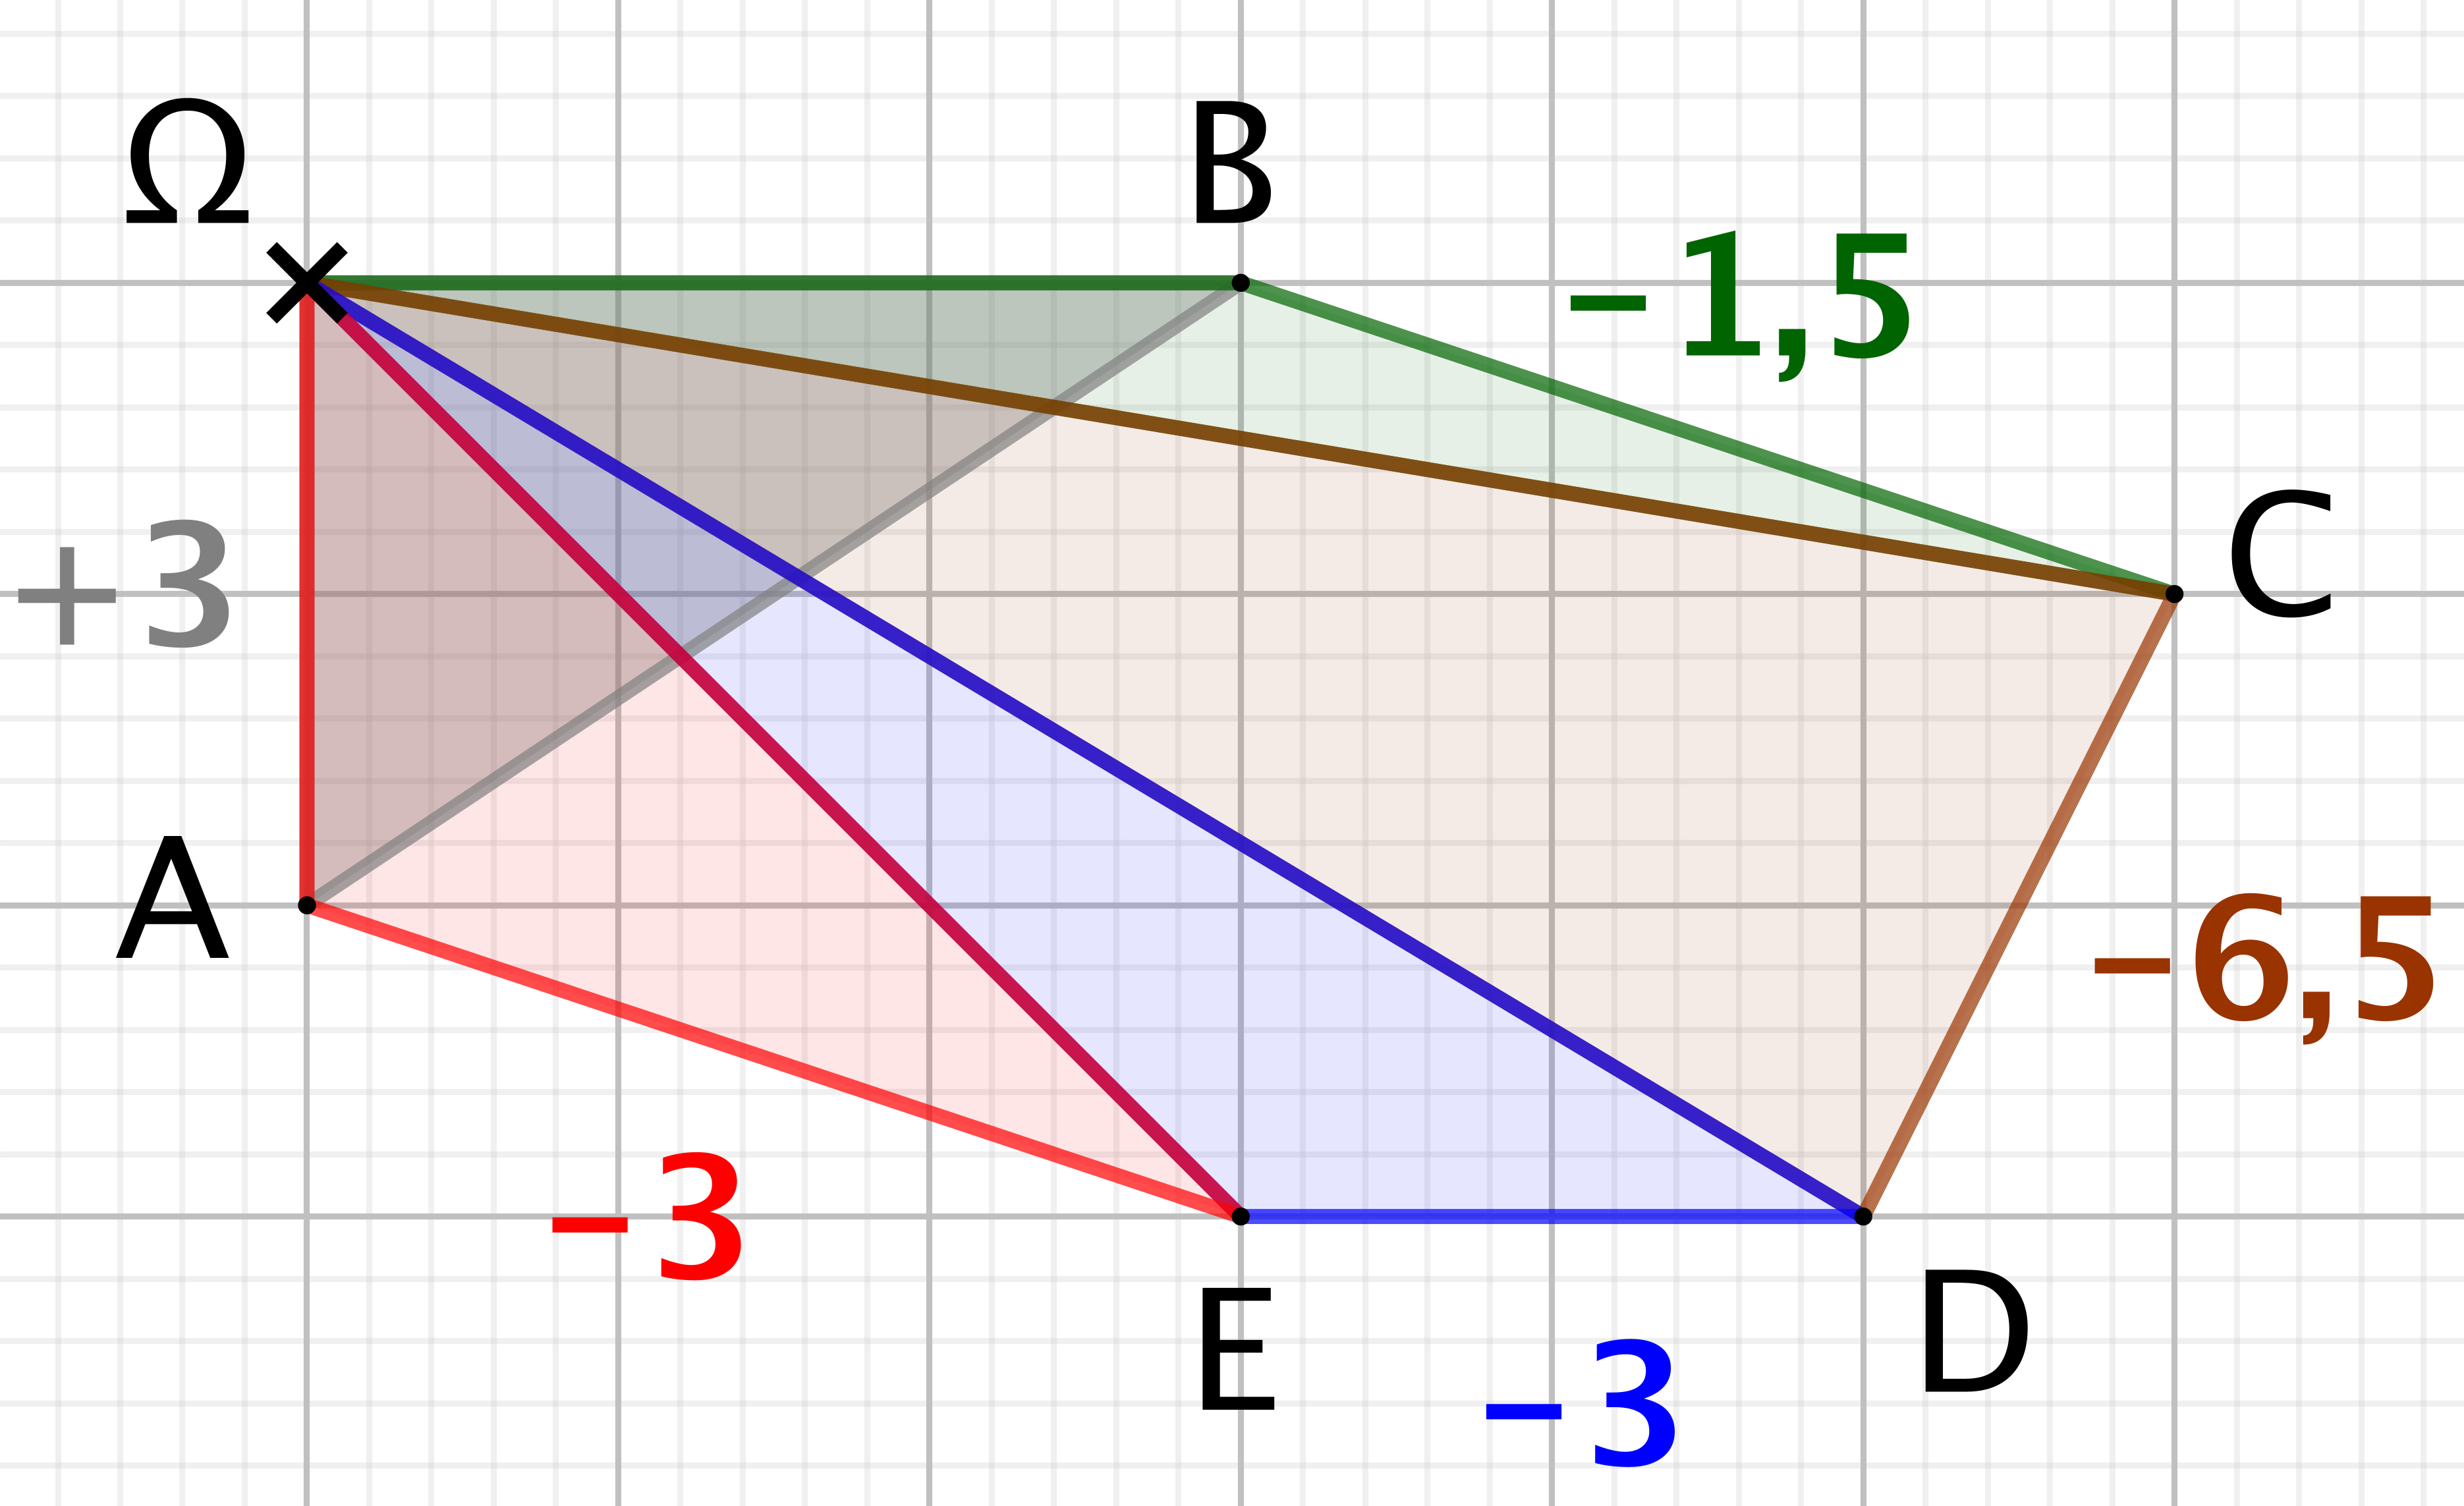
\includegraphics[scale=.35]{content/polygon/alg-area/convex-2.png}

       	\smallskip

		$- 11 = 3 - \num{1.5} - \num{6.5} - 3 - 3 \vphantom{\dfrac{2^M}2}$
    \end{center}
\end{multicols}


Dans le cas précédent, le résultat pourrait dépendre du point $\Omega$ employé, mais le fait suivant nous montre que non. Bonne nouvelle! Yapluka...


% ----------------------- %


\begin{fact} \label{sarea-pt-ct}
    Soit $\setproba{L} = A_1 A_2 \cdots A_n$ un \ncycle\ où $n \geq 2$.
    La fonction qui à un point $\Omega$ du plan associe
    $\mu_1^n (\Omega ;\setproba{L}) = \dsum_{i=1}^{n} \det \big( \vect{\Omega A^{\,\prime}_i} , \vect{\Omega A^{\,\prime}_{i+1}} \big)$ est indépendante du point $\Omega$.
    Dans la suite, cette quantité indépendante de $\Omega$ sera notée $\mu_1^n (\setproba{L})$.
\end{fact}


\begin{proof}
    Soit $M$ un autre point du plan.

    \begin{stepcalc}[style=ar*]
        \mu_1^n (\Omega ;\setproba{L})
    \explnext{}
        \dsum_{i=1}^{n} \det \big( \vect{\Omega A^{\,\prime}_i} , \vect{\Omega A^{\,\prime}_{i+1}} \big)
    \explnext{}
        \dsum_{i=1}^{n} \det \big( \vect{\Omega M} + \vect{M A^{\,\prime}_i} , \vect{\Omega M} + \vect{M A^{\,\prime}_{i+1}} \big)
    \explnext{}
        \dsum_{i=1}^{n} \Big[
            \det \big( \vect{\Omega M} , \vect{\Omega M} \big)
            +
            \det \big( \vect{\Omega M} , \vect{M A^{\,\prime}_{i+1}} \big)
            +
            \det \big( \vect{M A^{\,\prime}_i} , \vect{\Omega M} \big)
            +
            \det \big( \vect{M A^{\,\prime}_i} , \vect{M A^{\,\prime}_{i+1}} \big)
        \Big]
    \explnext{}
        \dsum_{i=1}^{n} \det \big( \vect{\Omega M} , \vect{M A^{\,\prime}_{i+1}} \big)
        +
        \dsum_{i=1}^{n} \det \big( \vect{M A^{\,\prime}_i} , \vect{\Omega M} \big)
        +
        \mu_1^n (M ; \setproba{L})
    \explnext{}
        \mu_1^n (M ; \setproba{L})
        +
        \dsum_{i=2}^{n+1} \det \big( \vect{\Omega M} , \vect{M A^{\,\prime}_{i}} \big)
        -
        \dsum_{i=1}^{n} \det \big( \vect{\Omega M} , \vect{M A^{\,\prime}_i} \big)
    \explnext*{$A^{\,\prime}_{n+1} = A^{\,\prime}_1$}{}
        \mu_1^n (M ; \setproba{L})
    \end{stepcalc}

    \null\vspace{-3.5ex}
\end{proof}


% ----------------------- %


\begin{fact} \label{nline-shift-inva}
    Soit $\setproba{L} = A_1 A_2 \cdots A_n$ un \ncycle\ où $n \geq 2$.
    Pour $k \in \ZintervalC{1}{n}$,
    définissant le \ncycle\ $\setproba{L}_k = B_1 B_2 \cdots B_n$ par $B_i = A^{\,\prime}_{i+k-1}$,
    nous avons
    $\mu_1^n (\setproba{L}) = \mu_1^n (\setproba{L}_k)$.
    Dans la suite, cette quantité commune sera notée $\mu (\setproba{L})$.
\end{fact}


\begin{proof}
    Il suffit de s'adonner à un petit jeu sur les indices de sommation.
\end{proof}


% ----------------------- %


\begin{fact} \label{nline-rota-opp}
    Soit
    $\setproba{L} = A_1 A_2 \cdots A_n$ un \ncycle\ où $n \geq 2$.
    Le \ncycle\ \og \emph{opposé} \fg\ $\setproba{L}^{\mathrm{op}} = B_1 B_2 \cdots B_n$, où $B_i =  A_{n + 1 - i}$,
    vérifie
    $\mu(\setproba{L}^{\mathrm{op}}) = {} - \mu(\setproba{L})$.
\end{fact}


\begin{proof}
    Soit $\Omega$ un point quelconque du plan.

    \begin{stepcalc}[style=ar*]
        \mu(\setproba{L}^{\mathrm{op}})
    \explnext{}
        \dsum_{i=1}^{n} \det \big( \vect{\Omega B^{\,\prime}_i} , \vect{\Omega B^{\,\prime}_{i+1}} \big)
    \explnext*{$B^{\,\prime}_i =  A^{\,\prime}_{n + 1 - i}$ et $j = n - i$}{}
%        \dsum_{i=1}^{n} \det \big( \vect{\Omega A^{\,\prime}_{n + 1 - i}} , \vect{\Omega A^{\,\prime}_{n - i}} \big)
%    \explnext{}
        \dsum_{j=0}^{n-1} \det \big( \vect{\Omega A^{\,\prime}_{j + 1}} , \vect{\Omega A^{\,\prime}_j} \big)
    \explnext*{$A^{\,\prime}_0 = A^{\,\prime}_n$ et $A^{\,\prime}_1 = A^{\,\prime}_{n+1}$}{}
%        \dsum_{j=1}^{n} \det \big( \vect{\Omega A^{\,\prime}_{j + 1}} , \vect{\Omega A^{\,\prime}_j} \big)
%    \explnext{}
        {} - \dsum_{j=1}^{n} \det \big( \vect{\Omega A^{\,\prime}_j} , \vect{\Omega A^{\,\prime}_{j + 1}} \big)
    \explnext{}
        {} - \mu(\setproba{L})
    \end{stepcalc}

    \null\vspace{-3.5ex}
\end{proof}


% ----------------------- %


\begin{fact} \label{sarea-ncycle}
    Soit
    $\setproba{L} = A_1 A_2 \cdots A_n$ un \ncycle\ où $n \geq 2$.
    La quantité $\sarea{\setproba{L}} = \frac12 \mu(\setproba{L})$ ne dépend que du sens de parcours de $\setproba{L}$, mais pas du point de départ.%
    \footnote{
        Le lecteur pardonnera les abus de langage utilisés.
    }
    Elle sera appelée \og \emph{aire algébrique} \fg\ de $\setproba{L}$, et elle est étendue au \xcycle{0} et aux \xcycles{1} par $\sarea{\setproba{L}} = 0$ pour ces cycles particuliers.
\end{fact}


\begin{proof}
    C'est une conséquence directe des faits \ref{nline-shift-inva} et \ref{nline-rota-opp}.
\end{proof}


% ----------------------- %


Considérons, maintenant, un \ngone\ convexe $\setproba{P} = A_1 A_2 \cdots A_n$ où les sommets sont parcourus dans le sens anti-horaire.
En choisissant l'isobarycentre $G$ des points $A_1$, $A_2$, ..., $A_n$ pour le calcul de $\sarea{\setproba{P}}$, nous obtenons que $\area{\setproba{P}} = \sarea{\setproba{P}}$:
en effet,
avec ce choix, tous les déterminants $\det \big( \vect{G A^{\,\prime}_i} , \vect{G A^{\,\prime}_{i+1}} \big)$ sont positifs.
Dans le cas non-convexe, les choses se compliquent a priori, car nous ne maîtrisons plus les signes des déterminants. Heureusement, nous avons le résultat essentiel suivant.


\begin{fact} \label{route-direction}
    Soit un \ngone\ $\setproba{P} = A_1 A_2 \cdots A_n$ tel que $A_1$, $A_2$, ..., $A_n$ soient parcourus dans le sens trigonométrique, ou anti-horaire.
    Un tel \ngone\ sera dit \og \emph{positif} \fg.%
    \footnote{
    	Bien noté que cette notion ne peut pas exister pour un \ngone\ croisé. De façon cachée, nous utilisons le célèbre théorème de Jordan, dans sa forme polygonale.
    }
    Sous cette hypothèse, nous avons 
    $\mu(\setproba{P}) \geq 0$,
    \emph{i.e.}
    $\sarea{\setproba{P}} \geq 0$.
\end{fact}


\begin{proof}
	Le théorème de triangulation affirme que tout \ngone\ est triangulable comme dans l'exemple suivant: ceci laisse envisager une démonstration par récurrence en retirant l'un des triangles ayant deux côtés correspondant à deux côtés consécutifs du \ngone\ (pour peu qu'un tel triangle existe toujours).


    \begin{multicols}{3}
        \small\itshape
        \begin{center}
            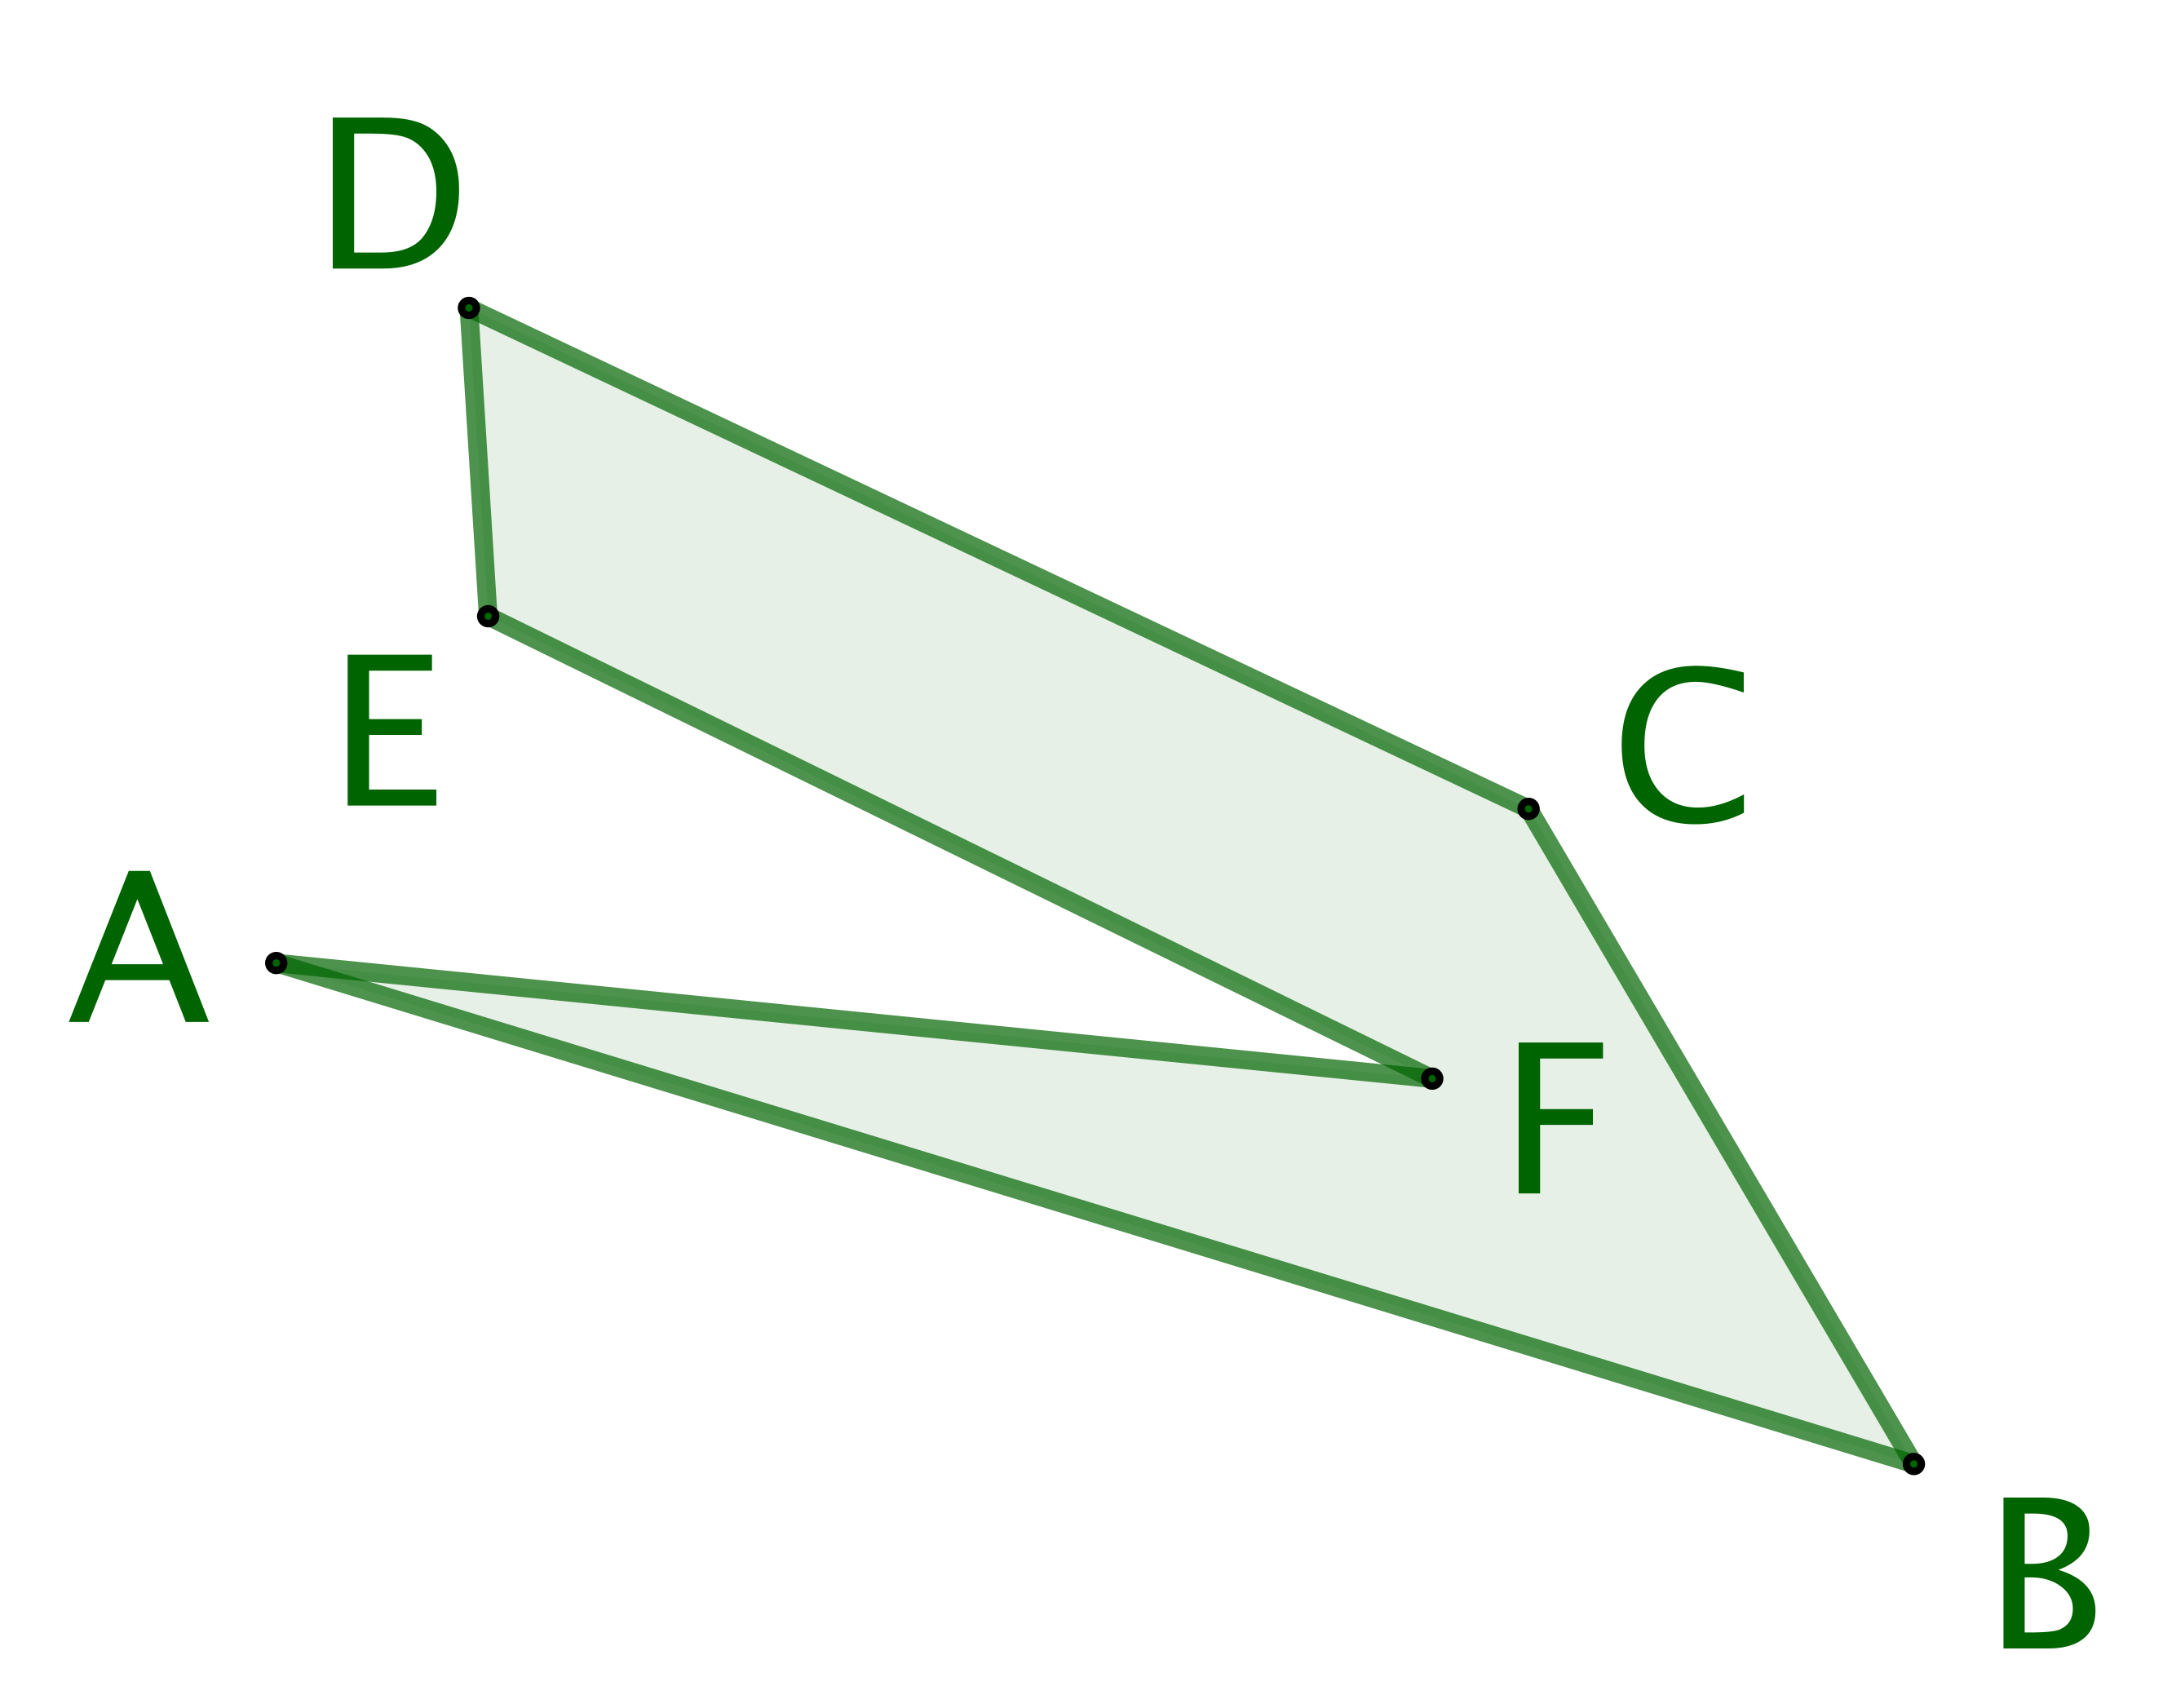
\includegraphics[scale=.4]{content/polygon/alg-area/triangulation-1.png}

            \smallskip
            Un \ngone\ \og nu \fg.
        \end{center}


        \begin{center}
            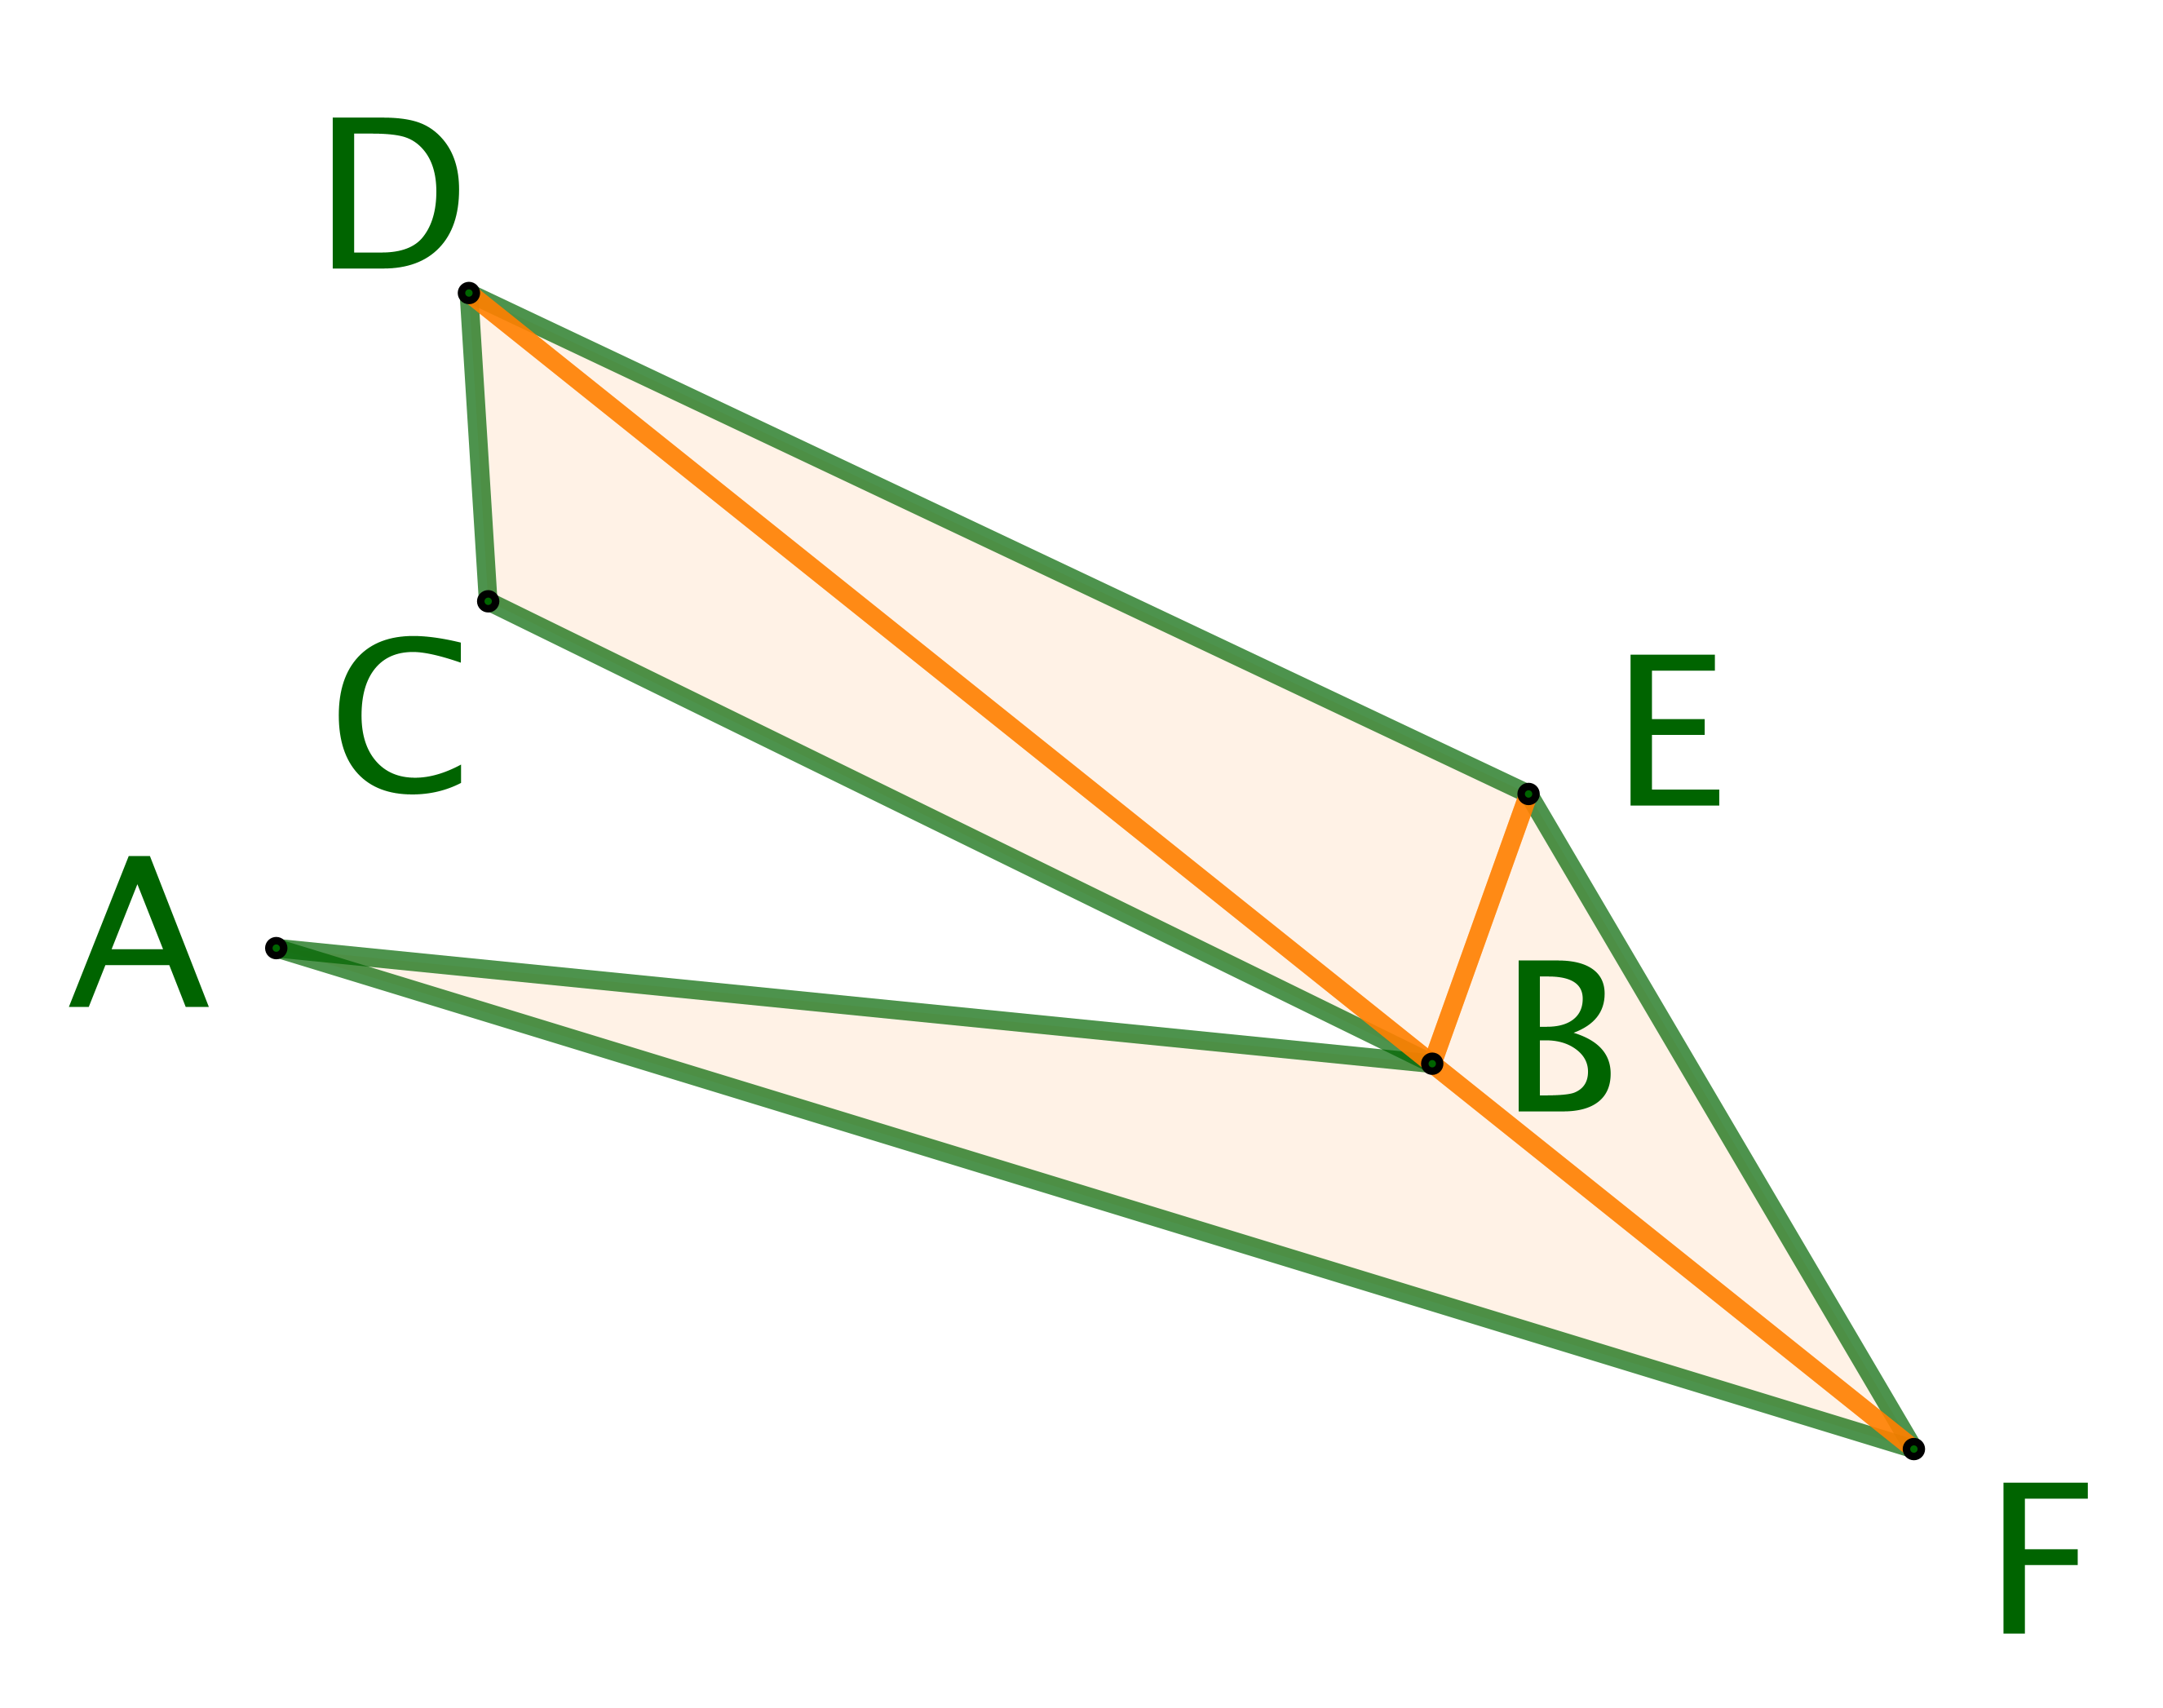
\includegraphics[scale=.4]{content/polygon/alg-area/triangulation-2.png}

            \smallskip
            Le \ngone\ triangulé.
        \end{center}


        \begin{center}
            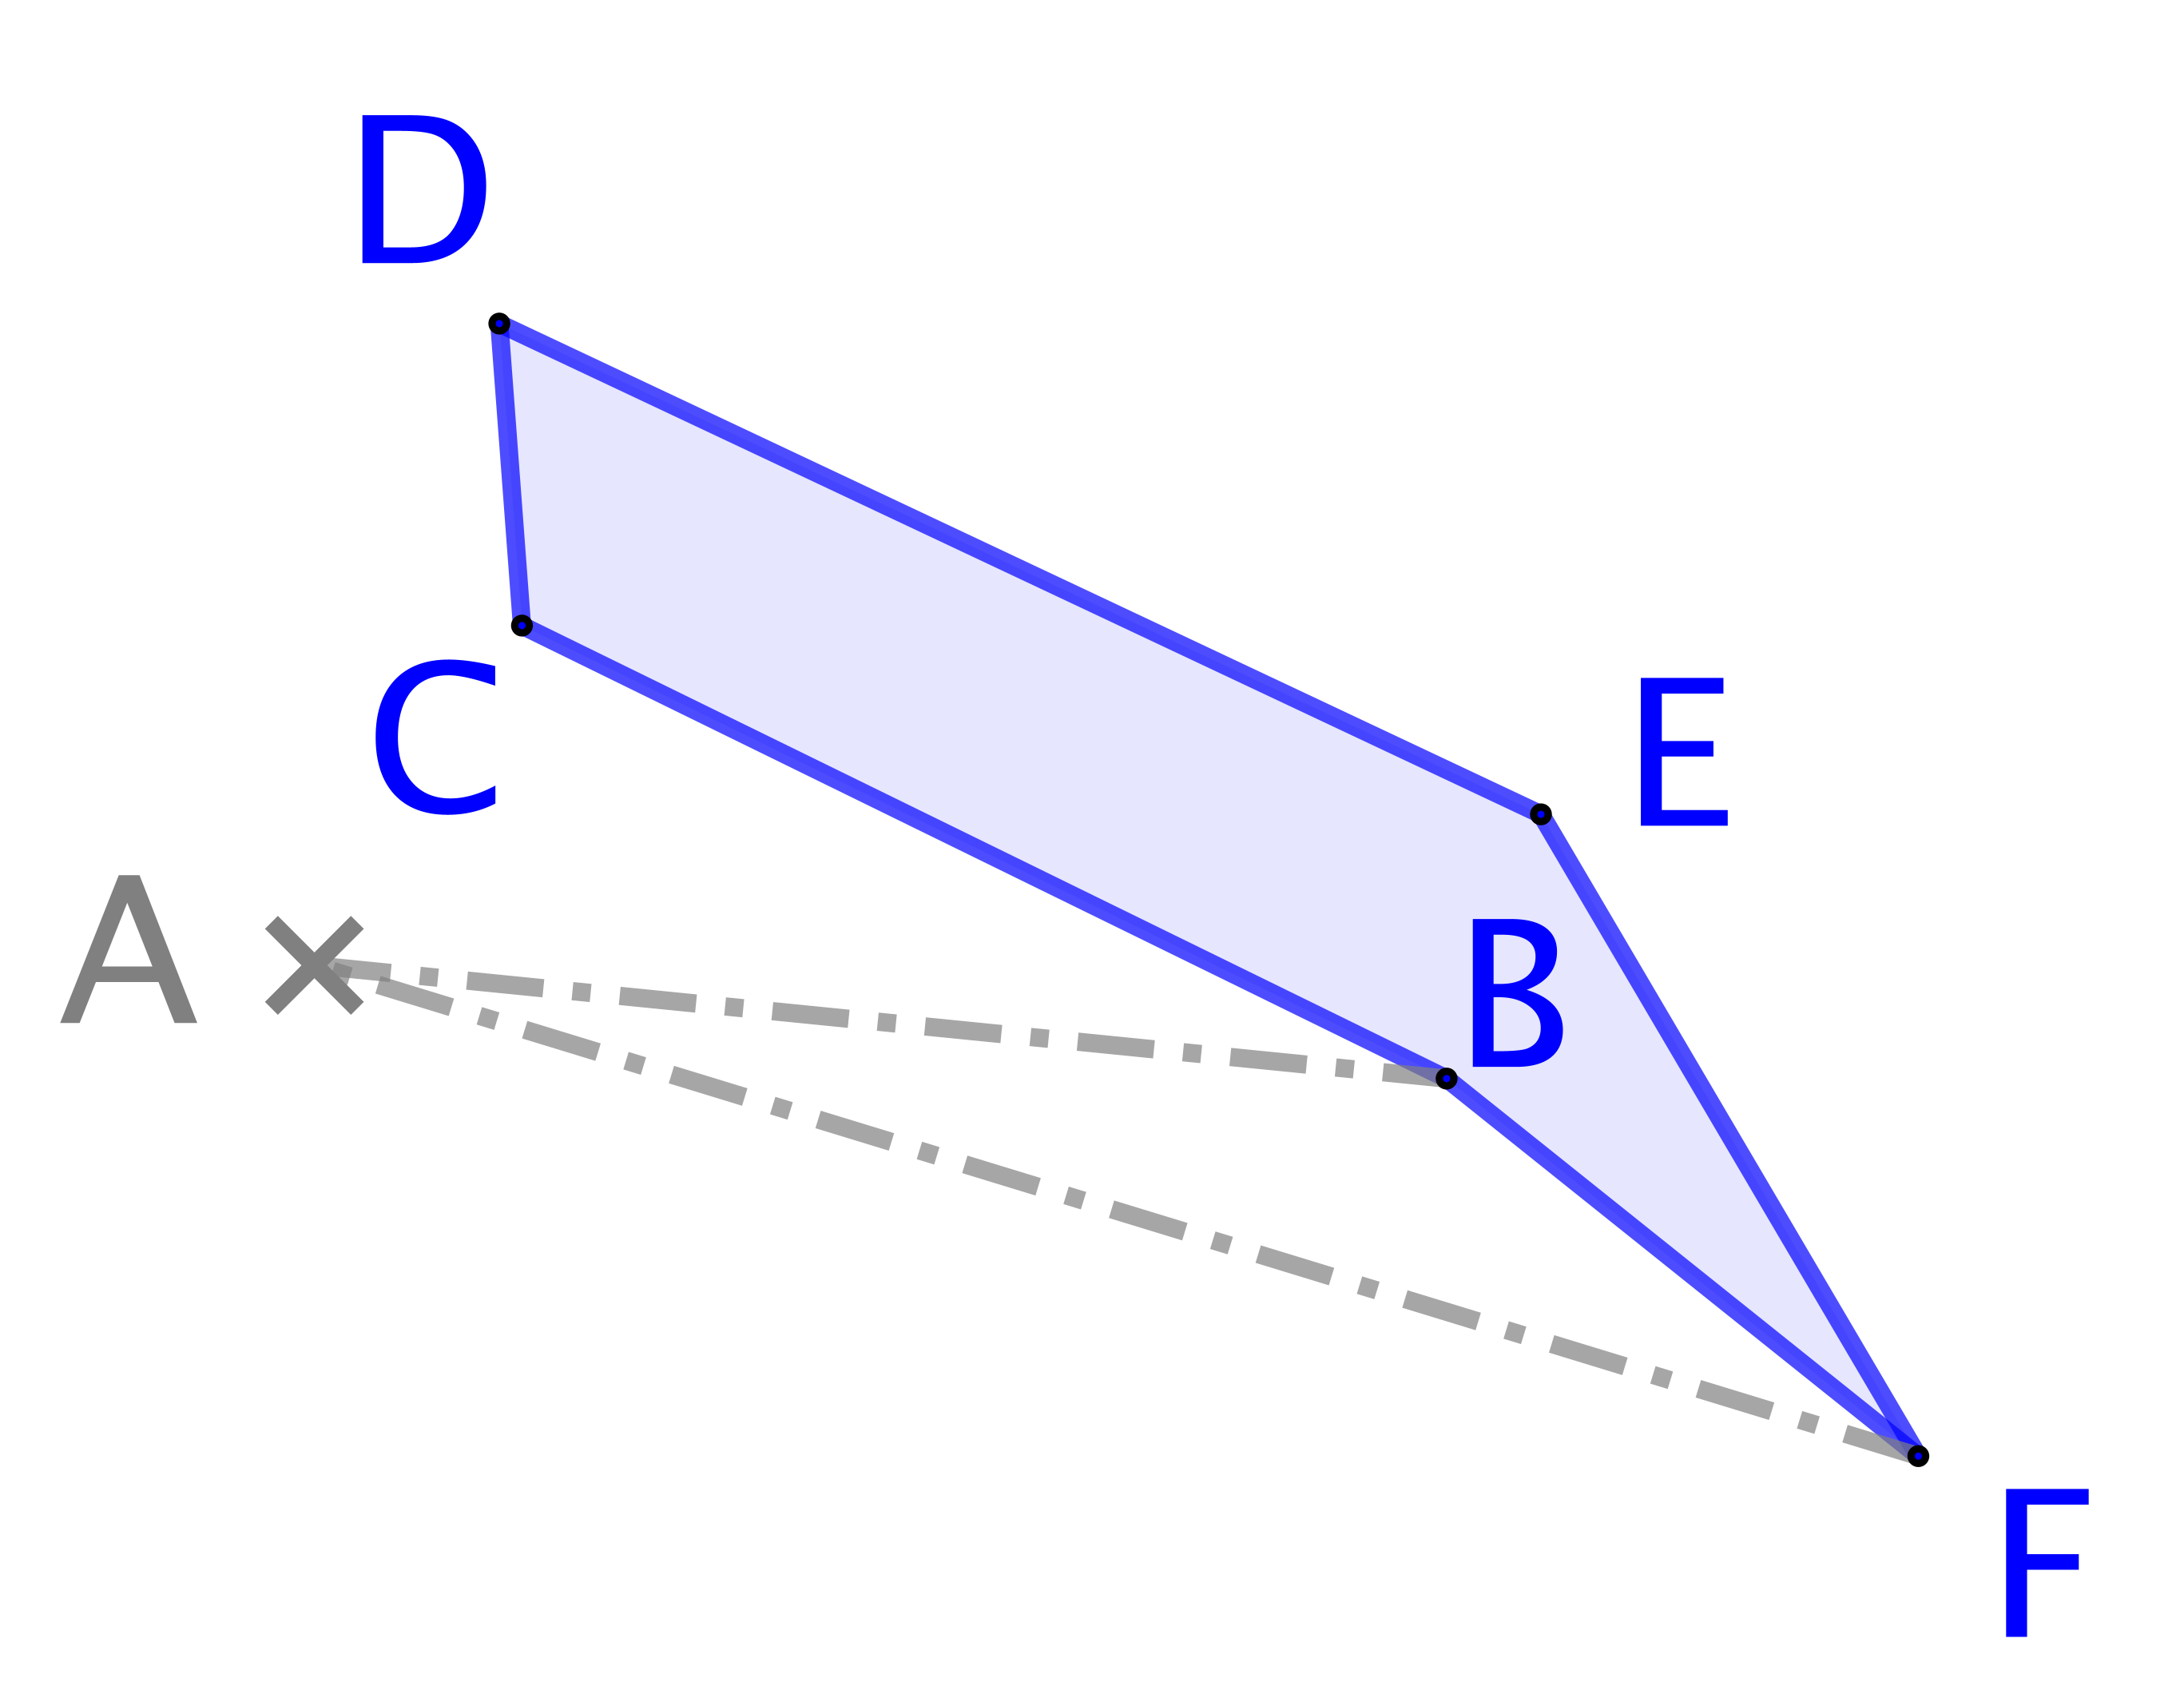
\includegraphics[scale=.4]{content/polygon/alg-area/triangulation-3.png}

            \smallskip
            Le \ngone\ allégé.
        \end{center}
    \end{multicols}


    Le théorème de triangulation admet une forme forte donnant une décomposition contenant un triangle formé de deux côtés consécutifs du \ngone.%
    \footnote{
        En pratique, cette forme forte est peu utile, car elle aboutit à un algorithme de recherche trop lent.
    }
    Nous dirons qu'une telle décomposition est \og \emph{à l'écoute} \fg.
    Ce très mauvais jeu de mots fait référence à la notion sérieuse \og \emph{d'oreille} \fg\ pour un \ngone: une oreille est un triangle inclus dans le \ngone, et formé de deux côtés consécutifs du \ngone.
    L'exemple suivant donne un \ngone\ n'ayant que deux oreilles.%
    \footnote{
        On démontre que tout \ngone\ admet au minimum deux oreilles.
    }


    \begin{multicols}{2}
        \small\itshape
    	\begin{center}
        	
\includegraphics[scale=.4]{content/polygon/alg-area/mini-ear-1.png}

        	\smallskip
       		Un \ngone\ basique.
    	\end{center}

    	\begin{center}
        	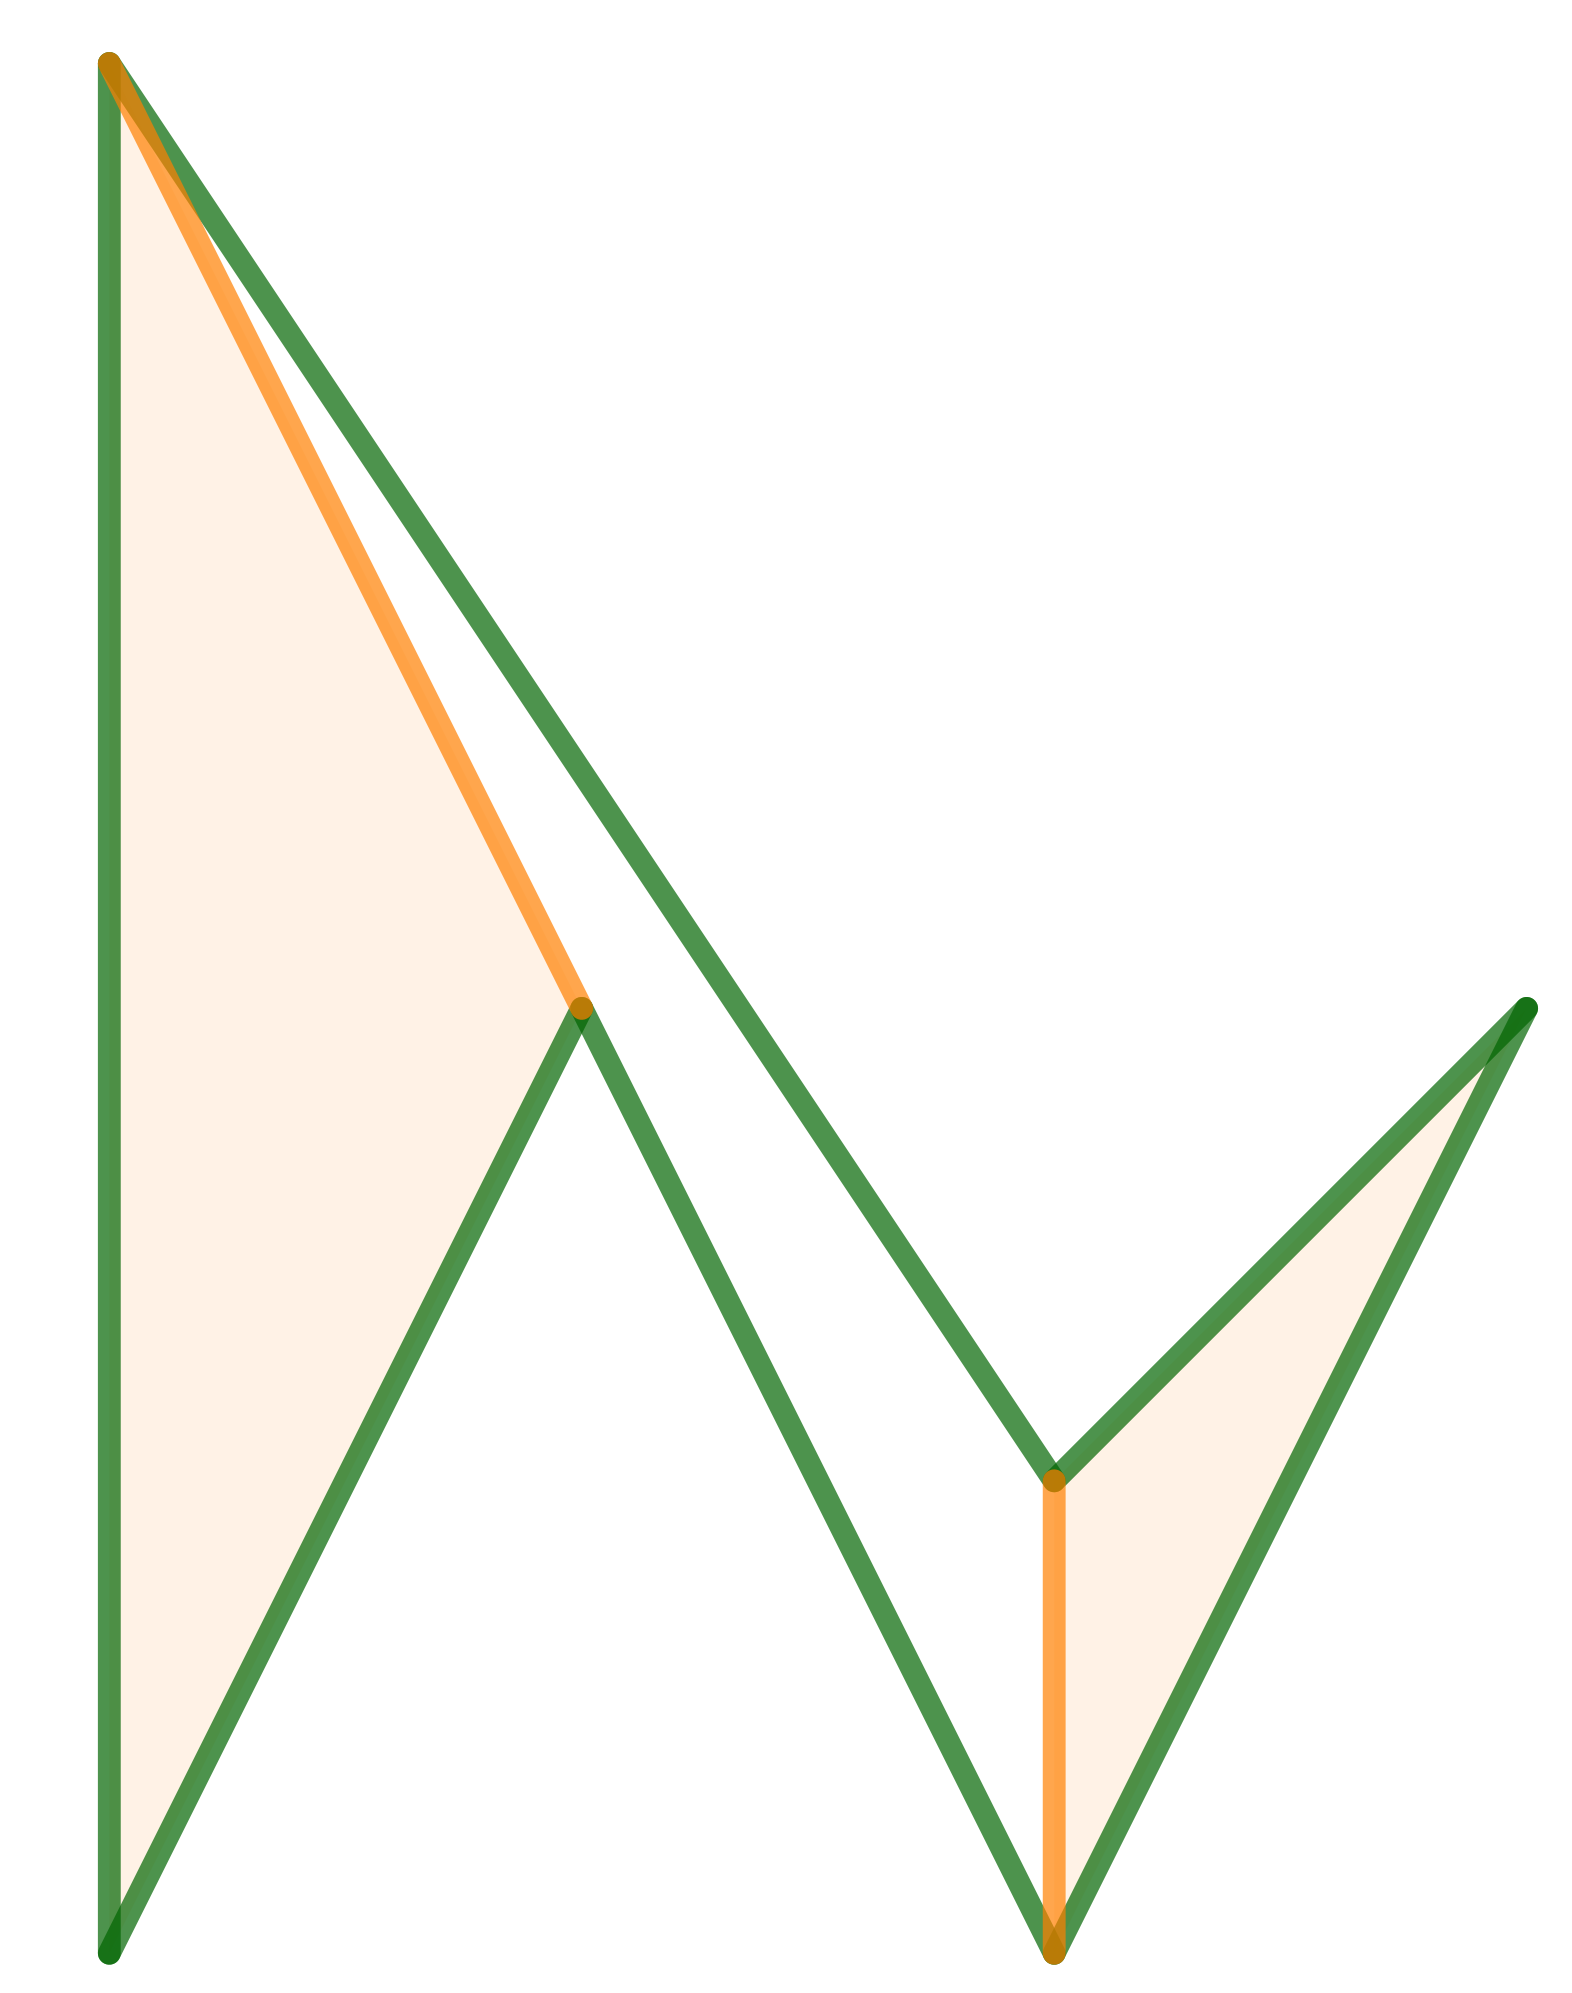
\includegraphics[scale=.4]{content/polygon/alg-area/mini-ear-2.png}

        	\smallskip
       		Juste deux oreilles disponibles.
    	\end{center}
    \end{multicols}


	Raisonnons donc par récurrence sur $n \in \NN_{\geq3}$.

	\begin{itemize}
		\item \textbf{Cas de base.}
		Soit $ABC$ un triangle. Dire que les sommets $A$, $B$ et $C$ sont parcourus dans le sens trigonométrique, c'est savoir que $\mu(ABC) = \det \big( \vect{AB} , \vect{AC} \big) > 0$.


		\item \textbf{Hérédité.}
		Soit un \ngone\ positif $\setproba{P} = A_1 A_2 \cdots A_n$ avec $n \in \NN_{>3}$. On peut supposer que $A_{n-1} A_n A_1$ est une oreille d'une triangulation à l'écoute du \ngone\ $\setproba{P}$.


	    \newpage
	    \begin{multicols}{2}
    	    \small\itshape
    		\begin{center}
        	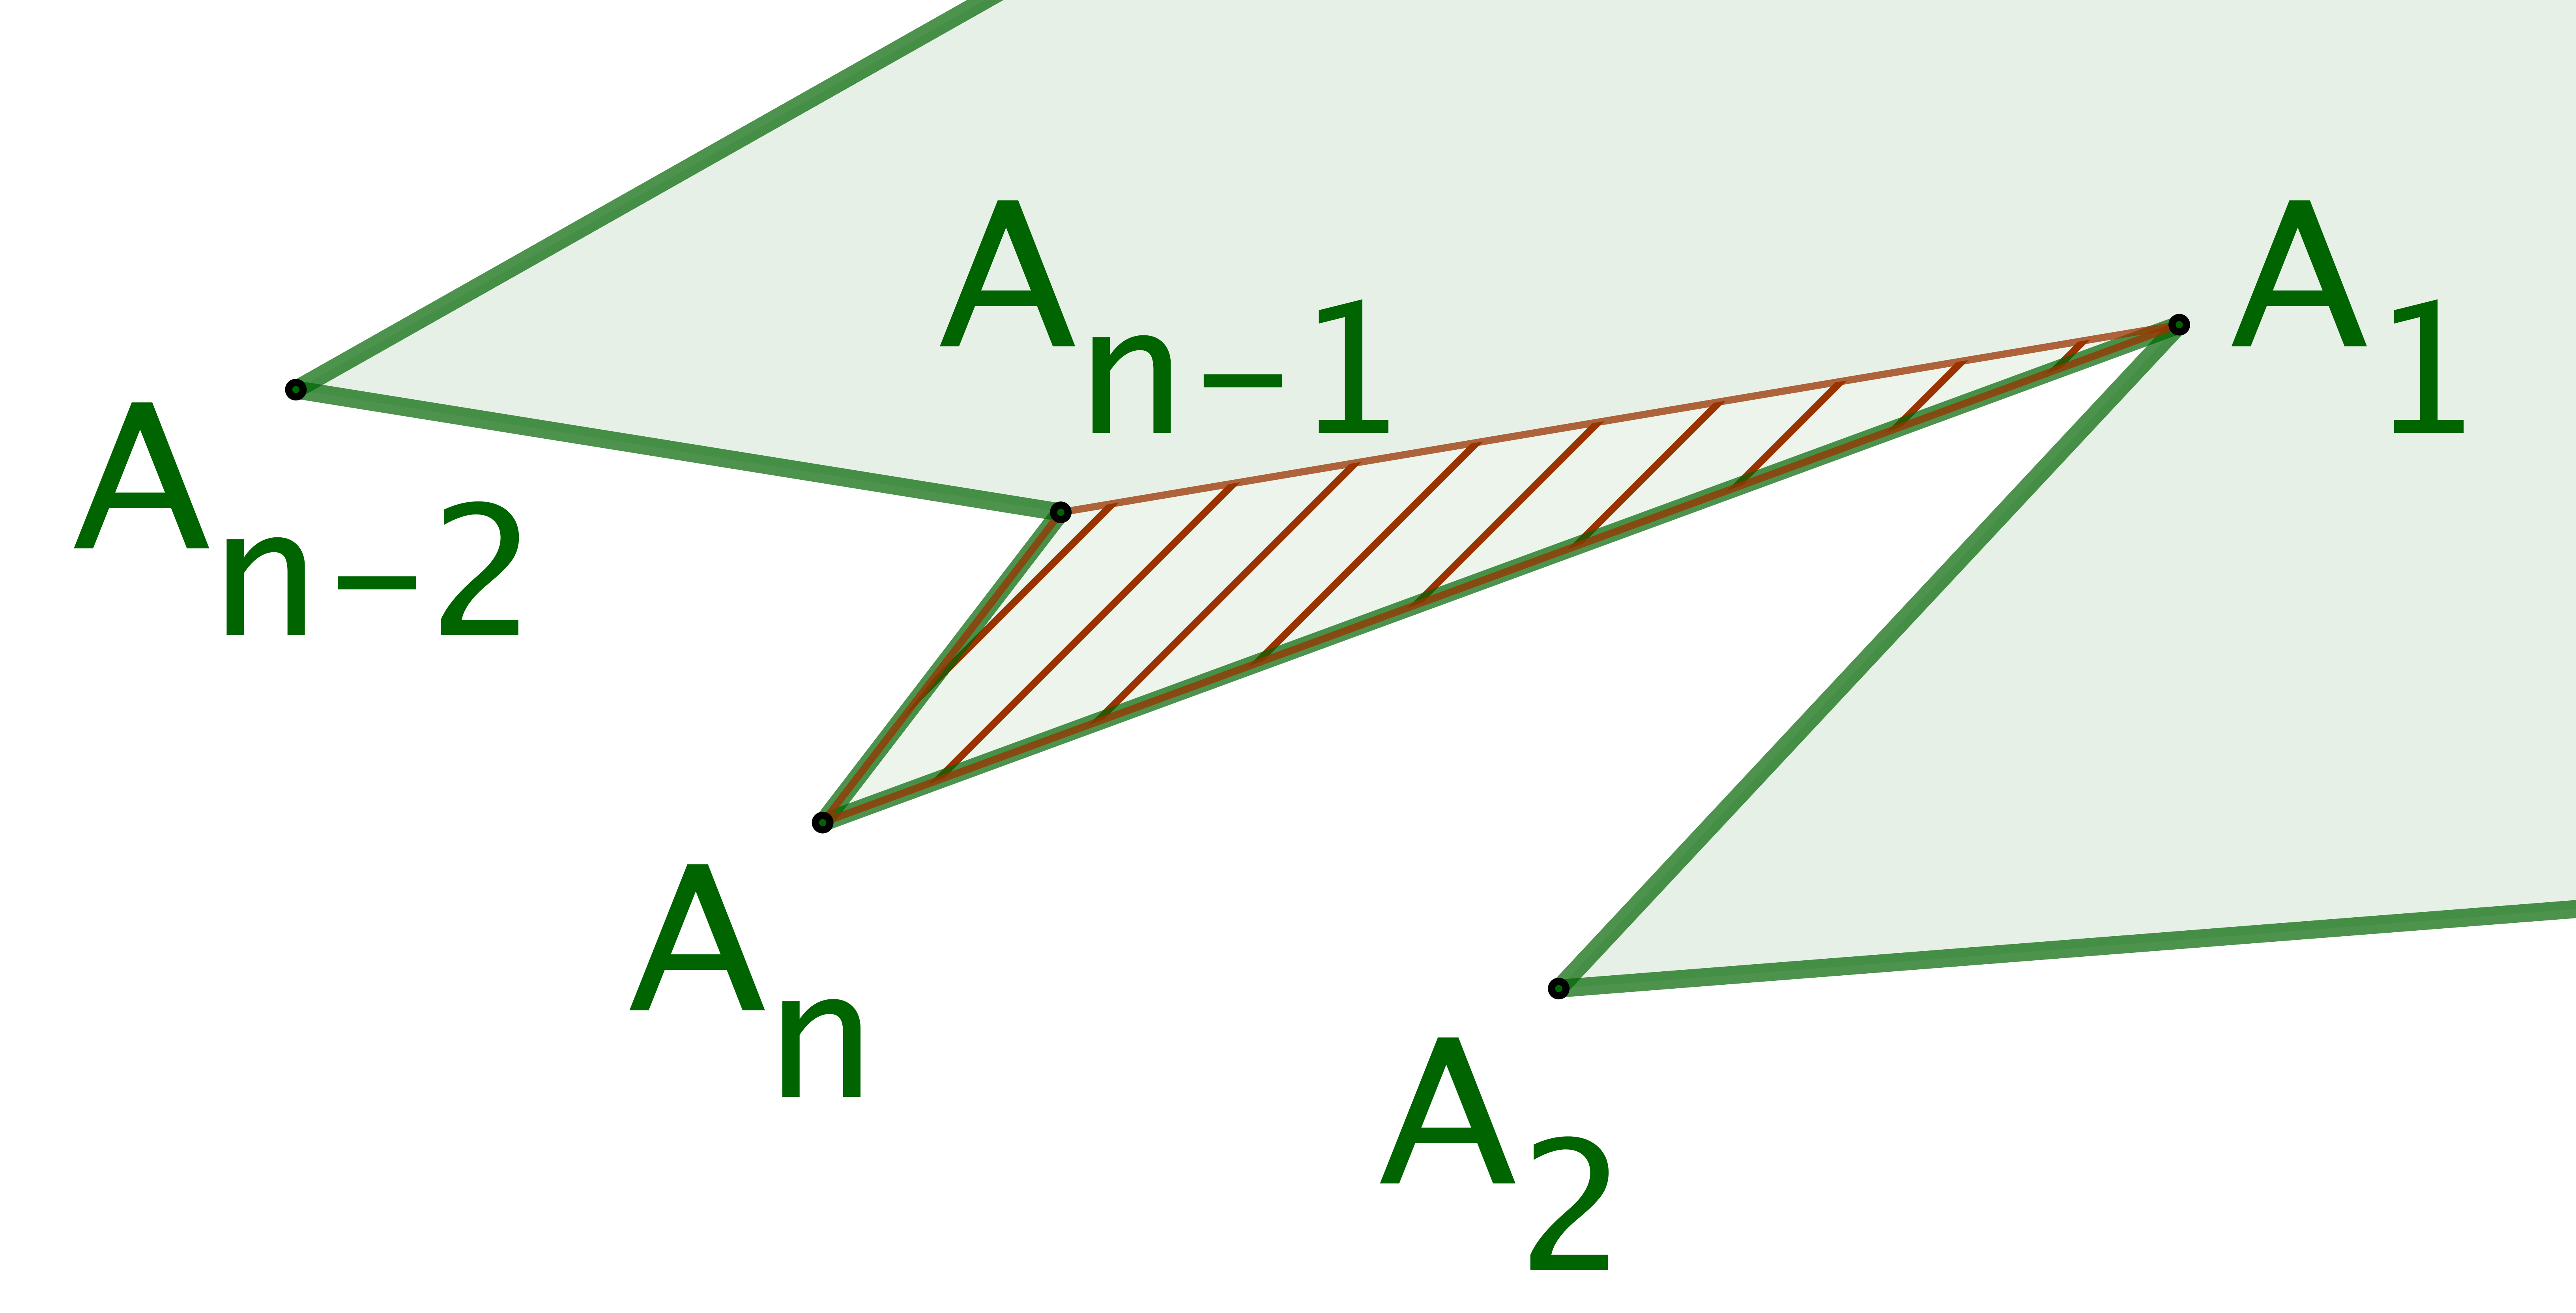
\includegraphics[scale=.4]{content/polygon/alg-area/triangulation-proof-OK.png}

	        	\smallskip
    	   		$A_{n-1} A_n A_1$ est une oreille.
    	\end{center}

	    	\begin{center}
        	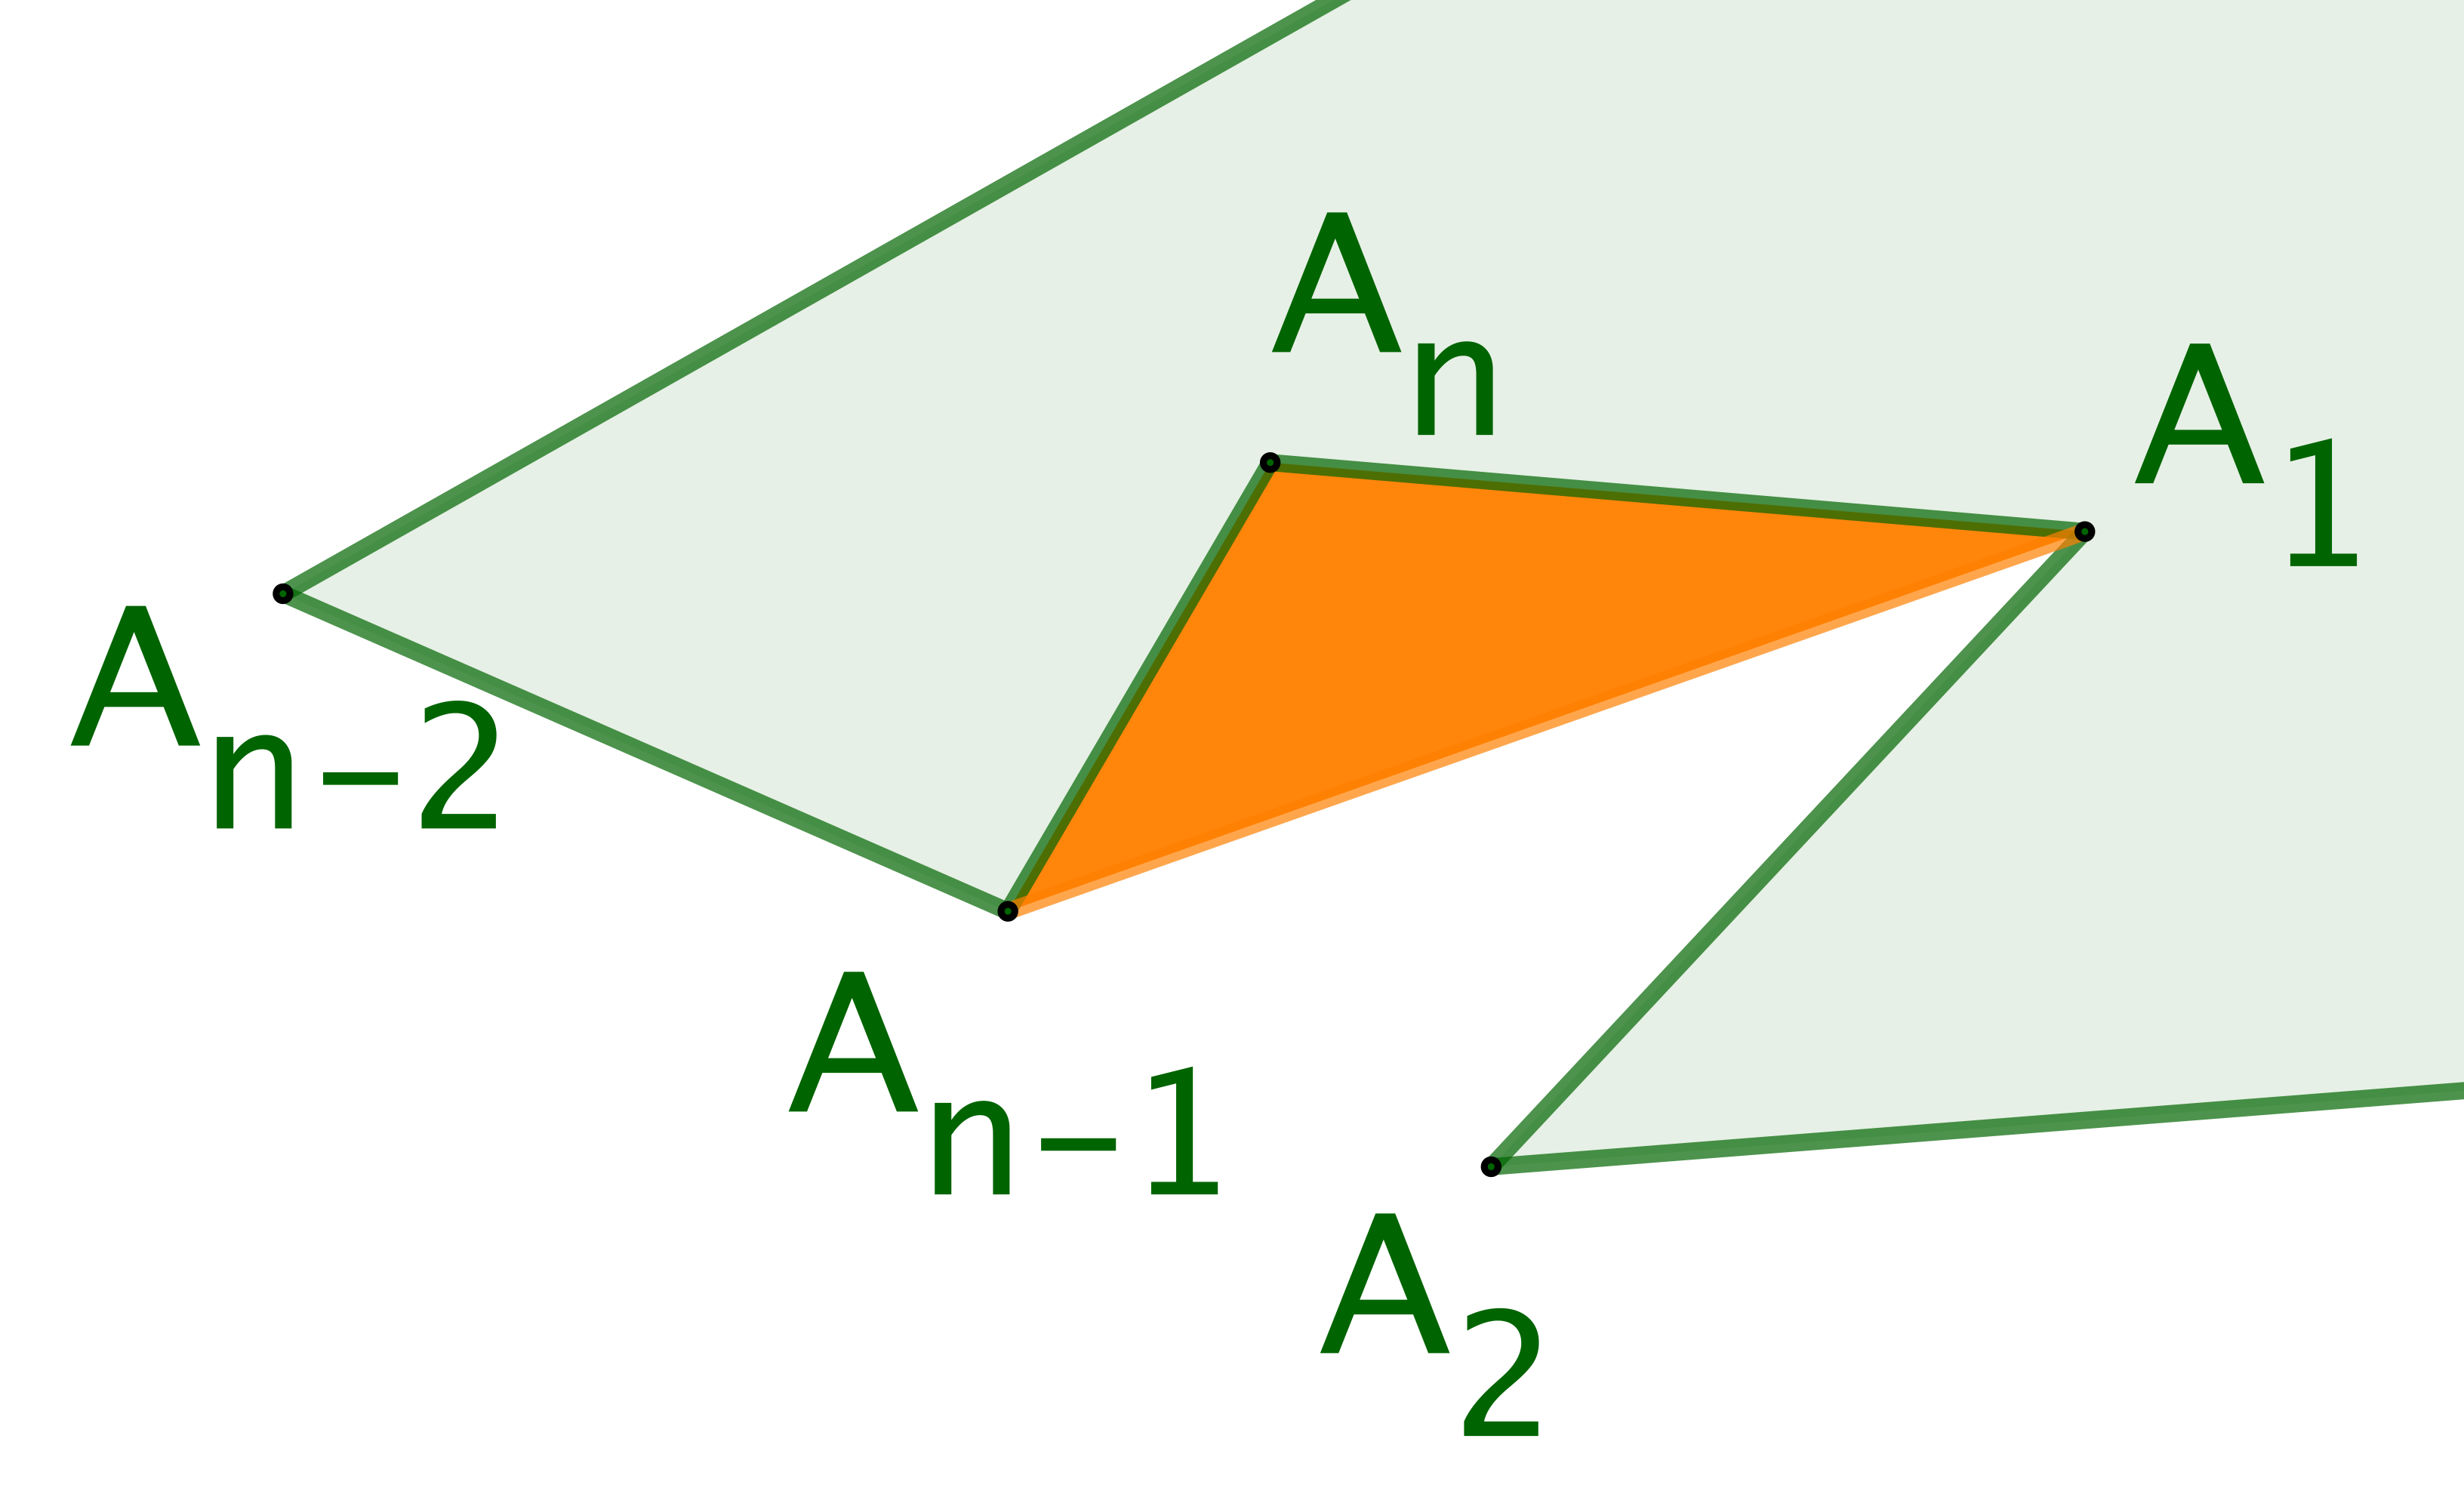
\includegraphics[scale=.4]{content/polygon/alg-area/triangulation-proof-KO.png}

        		\smallskip
    	   		$A_{n-1} A_n A_1$ n'est pas une oreille.
    		\end{center}
    	\end{multicols}


		\noindent
		Posons $\setproba{P}^{\,\prime} = A_1 \cdots A_{n-1}$ où $k = n-1$ vérifie $k \in \NN_{\geq3}$. Par hypothèse, $\setproba{P}^{\,\prime}$ est positif. 
		Nous arrivons finalement aux calculs élémentaires suivants en utilisant $A_1$ comme point de calcul de $\mu(\setproba{P})$.

		\leavevmode\kern-2em%
		\begin{stepcalc}[style=ar*]
			\mu(\setproba{P})
		%
%		\explnext{}
%			\dsum_{j=1}^{n} \det \big( \vect{A_1 A^{\,\prime}_j} , \vect{A_1 A^{\,\prime}_{j + 1}} \big)
%		%
		\explnext{}
			\dsum_{j=1}^{n} \det \big( \vect{A_1 A^{\,\prime}_j} , \vect{A_1 A^{\,\prime}_{j + 1}} \big)
%			+
%			\det \big( \vect{A_1 A^{\,\prime}_n} , \vect{A_1 A^{\,\prime}_{n+1}} \big)
		%
		\explnext*{$A^{\,\prime}_{n+1} = A_1$ \\
		           $A^{\,\prime}_i = A_i$ pour $i \leq n$}%
		          {}
			\dsum_{j=1}^{n-1} \det \big( \vect{A_1 A_j} , \vect{A_1 A_{j + 1}} \big)
%			+
%			\det \big( \vect{A_1 A_n} , \vect{A_1 A_1} \big)
		%
		\explnext{}
			\dsum_{j=1}^{n-2} \det \big( \vect{A_1 A_j} , \vect{A_1 A_{j + 1}} \big)
			+
			\det \big( \vect{A_1 A_{n-1}} , \vect{A_1 A_n} \big)
		%
		\explnext*{Pour $\mu(\setproba{P}^{\,\prime})$, noter que 
		        \\ $\det \big( \vect{A_1 A_{n-1}} , \vect{A_1 A_1} \big) = 0$.}{}
			\mu(\setproba{P}^{\,\prime})
			+
			\mu(A_{n-1} A_n A_1)
		\end{stepcalc}


		\noindent
		Par hypothèse de récurrence, nous savons que
		$\mu(\setproba{P}^{\,\prime}) \geq 0$,
		et comme $A_{n-1} A_n A_1$ est une oreille de $\setproba{P}$, la $3$-ligne $A_{n-1} A_n A_1$ est forcément positive, d'où $\mu(A_{n-1} A_n A_1) \geq 0$ d'après le cas de base.
		Nous arrivons bien à $\mu(\setproba{P}) \geq 0$, ce qui permet de finir aisément la démonstration par récurrence.
	\end{itemize}
	
	\null\vspace{-6ex}
\end{proof}


% ----------------------- %


\begin{fact} \label{sarea-ngone}
    Pour tout \ngone\ $\setproba{P}$, nous avons:
    $\area{\setproba{P}} = \abs{\sarea{\setproba{P}}}$.
\end{fact}


\begin{proof}
    Les deux points suivants permettent de faire une preuve par récurrence.

    \begin{itemize}
		\item \textbf{Cas de base.}
		L'égalité est immédiate pour les triangles (c'est ce qui a motivé la définition de l'aire algébrique).


		\item \textbf{Hérédité.}
		Soit $\setproba{P} = A_1 \cdots A_n$ un \ngone\ avec $n \in \NN_{>3}$.
		%
		Comme $\sarea{\setproba{P}^{\mathrm{op}}} = {} - \sarea{\setproba{P}}$ selon le fait \ref{nline-rota-opp}, nous pouvons choisir de parcourir $\setproba{P}$ positivement, puis de nous placer dans la situation de la démonstration du fait \ref{route-direction}:
		$A_{n-1} A_n A_1$ est une oreille positive d'une triangulation à l'écoute du \ngone\ $\setproba{P}$, et $\setproba{P}^{\,\prime} = A_1 \cdots A_{n-1}$ un \kgone\ positif où $k = n-1$ vérifie $k \in \NN_{\geq3}$.
		%
		Nous arrivons finalement aux calculs élémentaires suivants.
		
		\leavevmode\kern-2em%
		\begin{stepcalc}[style=ar*]
			\area{\setproba{P}}
		%
		\explnext*{$A_{n-1} A_n A_1$ est une oreille de $\setproba{P}$.}%
		          {}
		    \area{\setproba{P}^{\,\prime}} + \area{A_{n-1} A_n A_1}
		%
		\explnext*{Hypothèse de récurrence et cas de base.}%
		          {}
		    \frac12 \abs{\mu(\setproba{P}^{\,\prime})} + \frac12 \abs{\mu(A_{n-1} A_n A_1)}
		%
		\explnext*{Voir le fait \ref{route-direction}.}%
		          {}
		    \frac12 \big( \mu(\setproba{P}^{\,\prime}) + \mu(A_{n-1} A_n A_1) \big)
		%
		\explnext*{Comme dans la preuve du fait \ref{route-direction}.}%
		          {}
		    \frac12 \mu(\setproba{P})
		%
		\explnext*{Voir le fait \ref{route-direction}.}%
		          {}
		    \frac12 \abs{\mu(\setproba{P})}
		\explnext{}
		    \abs{\sarea{\setproba{P}}}
		\end{stepcalc}
    \end{itemize}
    
    \null\vspace{-3.5ex}
\end{proof}


% ----------------------- %


Finissons par un théorème de continuité qui permettra de justifier l'existence d'au moins une solution au problème d'isopérimétrie polygonale.


\begin{fact} \label{sarea-cont}
    Soient $n \in \NN_{\geq2}$ et
    $\pvaxes{O | i | j}$ un repère orthonormé direct du plan. 
    On note $\setproba{U} \subset \RR^{2n}$ l'ensemble des uplets de coordonnées $\big( x(A_1) ; y(A_1) ; \dots ; x(A_n) ; y(A_n) \big)$ où $A_1 A_2 \cdots A_n$ désigne un \ncycle,
    et $\alpha: \setproba{U} \rightarrow \RRp$ la fonction qui à un uplet de $\setproba{U}$ associe l'aire algébrique du \ncycle\ qu'il représente.
   	%
	Avec ces notations, la fonction $\alpha: \setproba{U} \rightarrow \RRp$ est continue.
\end{fact}


\begin{proof}
	Immédiat, car nous avons une fonction polynomiale.
\end{proof}

%
%
%\subsection{Au moins une solution, ou presque}
%\begin{fact} \label{suff-cond}
    Soit $n \in \NN_{\geq3}$ un naturel fixé.
    Parmi tous les \ncycles\ de longueur fixée, il en existe au moins un d'aire généralisée maximale.
\end{fact}


\begin{proof}
	Notons $\ell$ la longueur fixée que nous supposons non nulle.
	%
    \begin{itemize}
        \item Munissant le plan d'un repère orthonormé direct $\pvaxes{O | i | j}$, on note $\setproba{Z}$ l'ensemble des \ncycles\ $\setproba{L} = A_1 A_2 \cdots A_n$ tels que
        $\cyclelen{A_1 A_2 \cdots A_n} = \ell$
        et
        $A_1\coord{0 | 0}$,%
        \footnote{
        	Le mot \og \emph{Zeile} \fg\ est une traduction possible de \og \emph{ligne} \fg\ en allemand.
        }
        puis $\setproba{U} \subset \RR^{2n}$ l'ensemble des uplets de coordonnées $\big( x(A_1) ; y(A_1) ; \dots ; x(A_n) ; y(A_n) \big)$ pour $A_1 A_2 \cdots A_n \in \setproba{Z}$.


        \item $\setproba{U}$ est clairement fermé dans $\RR^{2n}$.
        De plus, il est borné, car les coordonnées des sommets des \ncycles\ considérés le sont.
        En résumé, $\setproba{U}$ est un compact de $\RR^{2n}$.


        \item Nous définissons la fonction $\alpha: \setproba{U} \rightarrow \RRp$ qui à un uplet de $\setproba{U}$ associe l'aire généralisée du \ncycle\ qu'il représente.
        Cette fonction est continue comme valeur absolue d'une fonction polynomiale en les coordonnées.


        \item Finalement, par continuité et compacité, $\alpha$ admet un maximum sur $\setproba{U}$.
    \end{itemize}
\end{proof}


% ----------------------- %


Comment le fait précédent peut-il nous aider dans notre quête d'un \ngone\ solution du problème d'isopérimétrie? Nous allons tout simplement démontré que tout \ncycle\ autre que le \ngone\ régulier ne peut pas être une solution \og optimale \fg.

%

\subsection{Solutions, qui êtes-vous?}
Cette section va établir que, relativement au problème d'isopérimétrie polygonal,
un \ngone\ solution doit être convexe, 
puis
qu'un \ngone\ convexe solution doit être un \nreg,
et enfin
que si $\setproba*{R}{1}$ et $\setproba*{R}{2}$ sont respectivement un \xgone{k_1} et un \xgone{k_2}, tous les deux réguliers convexes, avec 
$k_1 < k_2$ et $\perim{\setproba*{R}{1}} = \perim{\setproba*{R}{2}}$, 
alors
$\area{\setproba*{R}{1}} < \area{\setproba*{R}{2}}$.
Nous pourrons alors conclure dans la section finale suivante.


\begin{tcolorbox}
	\itshape\small
	Les cas $n = 3$ et $n = 4$ étant résolus, voir les faits \ref{iso-tri} et \ref{quadri}, dans toutes les preuves de cette section, nous supposerons $n \geq 5$, pour ne pas alourdir le texte.
\end{tcolorbox}


% ----------------------- %


\begin{fact} \label{must-be-conv}
    Pour tout \ngone\ non convexe $\setproba{P}$,
	nous pouvons construire un \ngone\ convexe $\setproba{C}$ tel que
	$\perim{\setproba{C}} = \perim{\setproba{P}}$
	et
	$\area{\setproba{C}} > \area{\setproba{P}}$.
\end{fact}


\begin{proof}
	Soit $\setproba{E}$ l'enveloppe convexe d'un \ngone\ non convexe $\setproba{P}$ (voir ci-dessous).
	
	\begin{center}
		\centering
		\small\itshape
		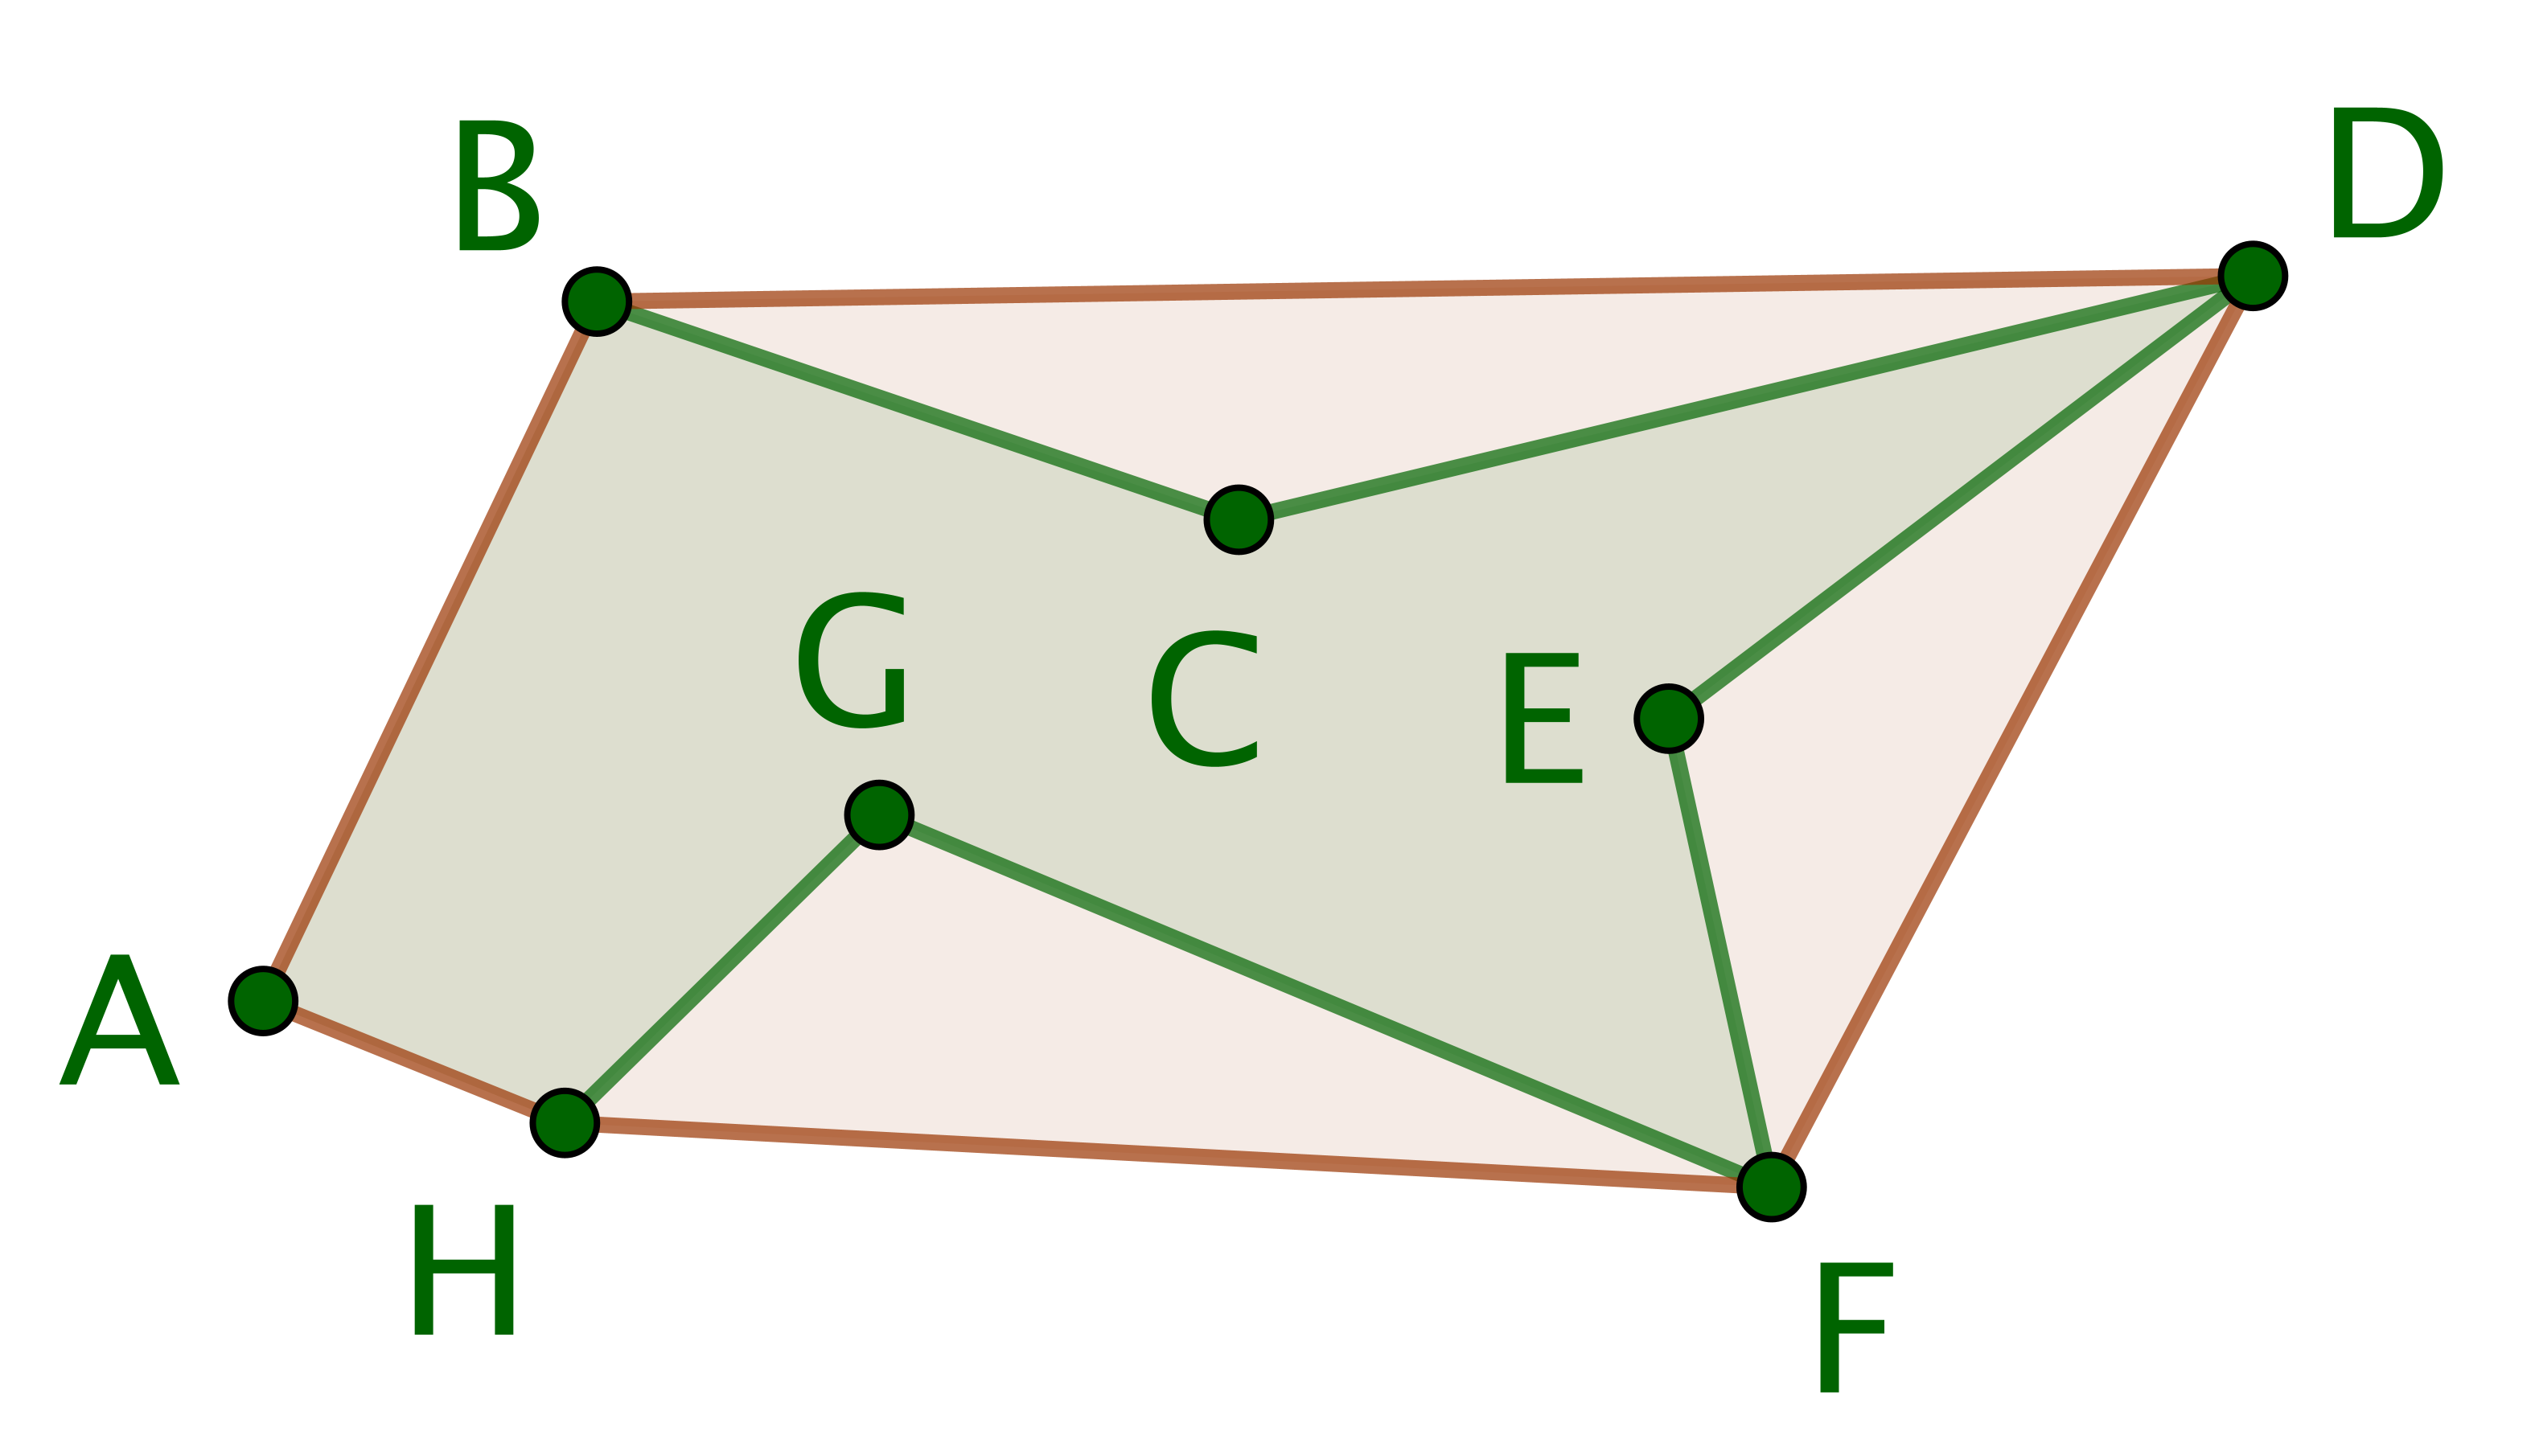
\includegraphics[scale=.45]{content/polygon/sol-must-be/convex-hull.png}
	\end{center}
	
		
	Clairement,
	$\perim{\setproba{E}} < \perim{\setproba{P}}$
	et
	$\area{\setproba{E}} > \area{\setproba{P}}$,
	mais
	$\setproba{E}$ est un \xgone{s} avec $s < n$. 
	%
	Pour gérer ce problème, une idée simple, formalisée après, est d'ajouter des sommets assez prêts des côtés de $\setproba{E}$ pour garder 
	la convexité, 
	un périmètre inférieur à $\perim{\setproba{P}}$, 
	et
	une aire supérieure à $\area{\setproba{P}}$.
	Si c'est faisable, une homothétie de rapport $r \geq 1$, où $r = \frac{ \perim{\setproba{P}} }{ \perim{\setproba{E}} }$, donnera le \ngone\ convexe $\setproba{C}$ cherché.
	La figure suivante illustre cette idée.
	
	\begin{center}
		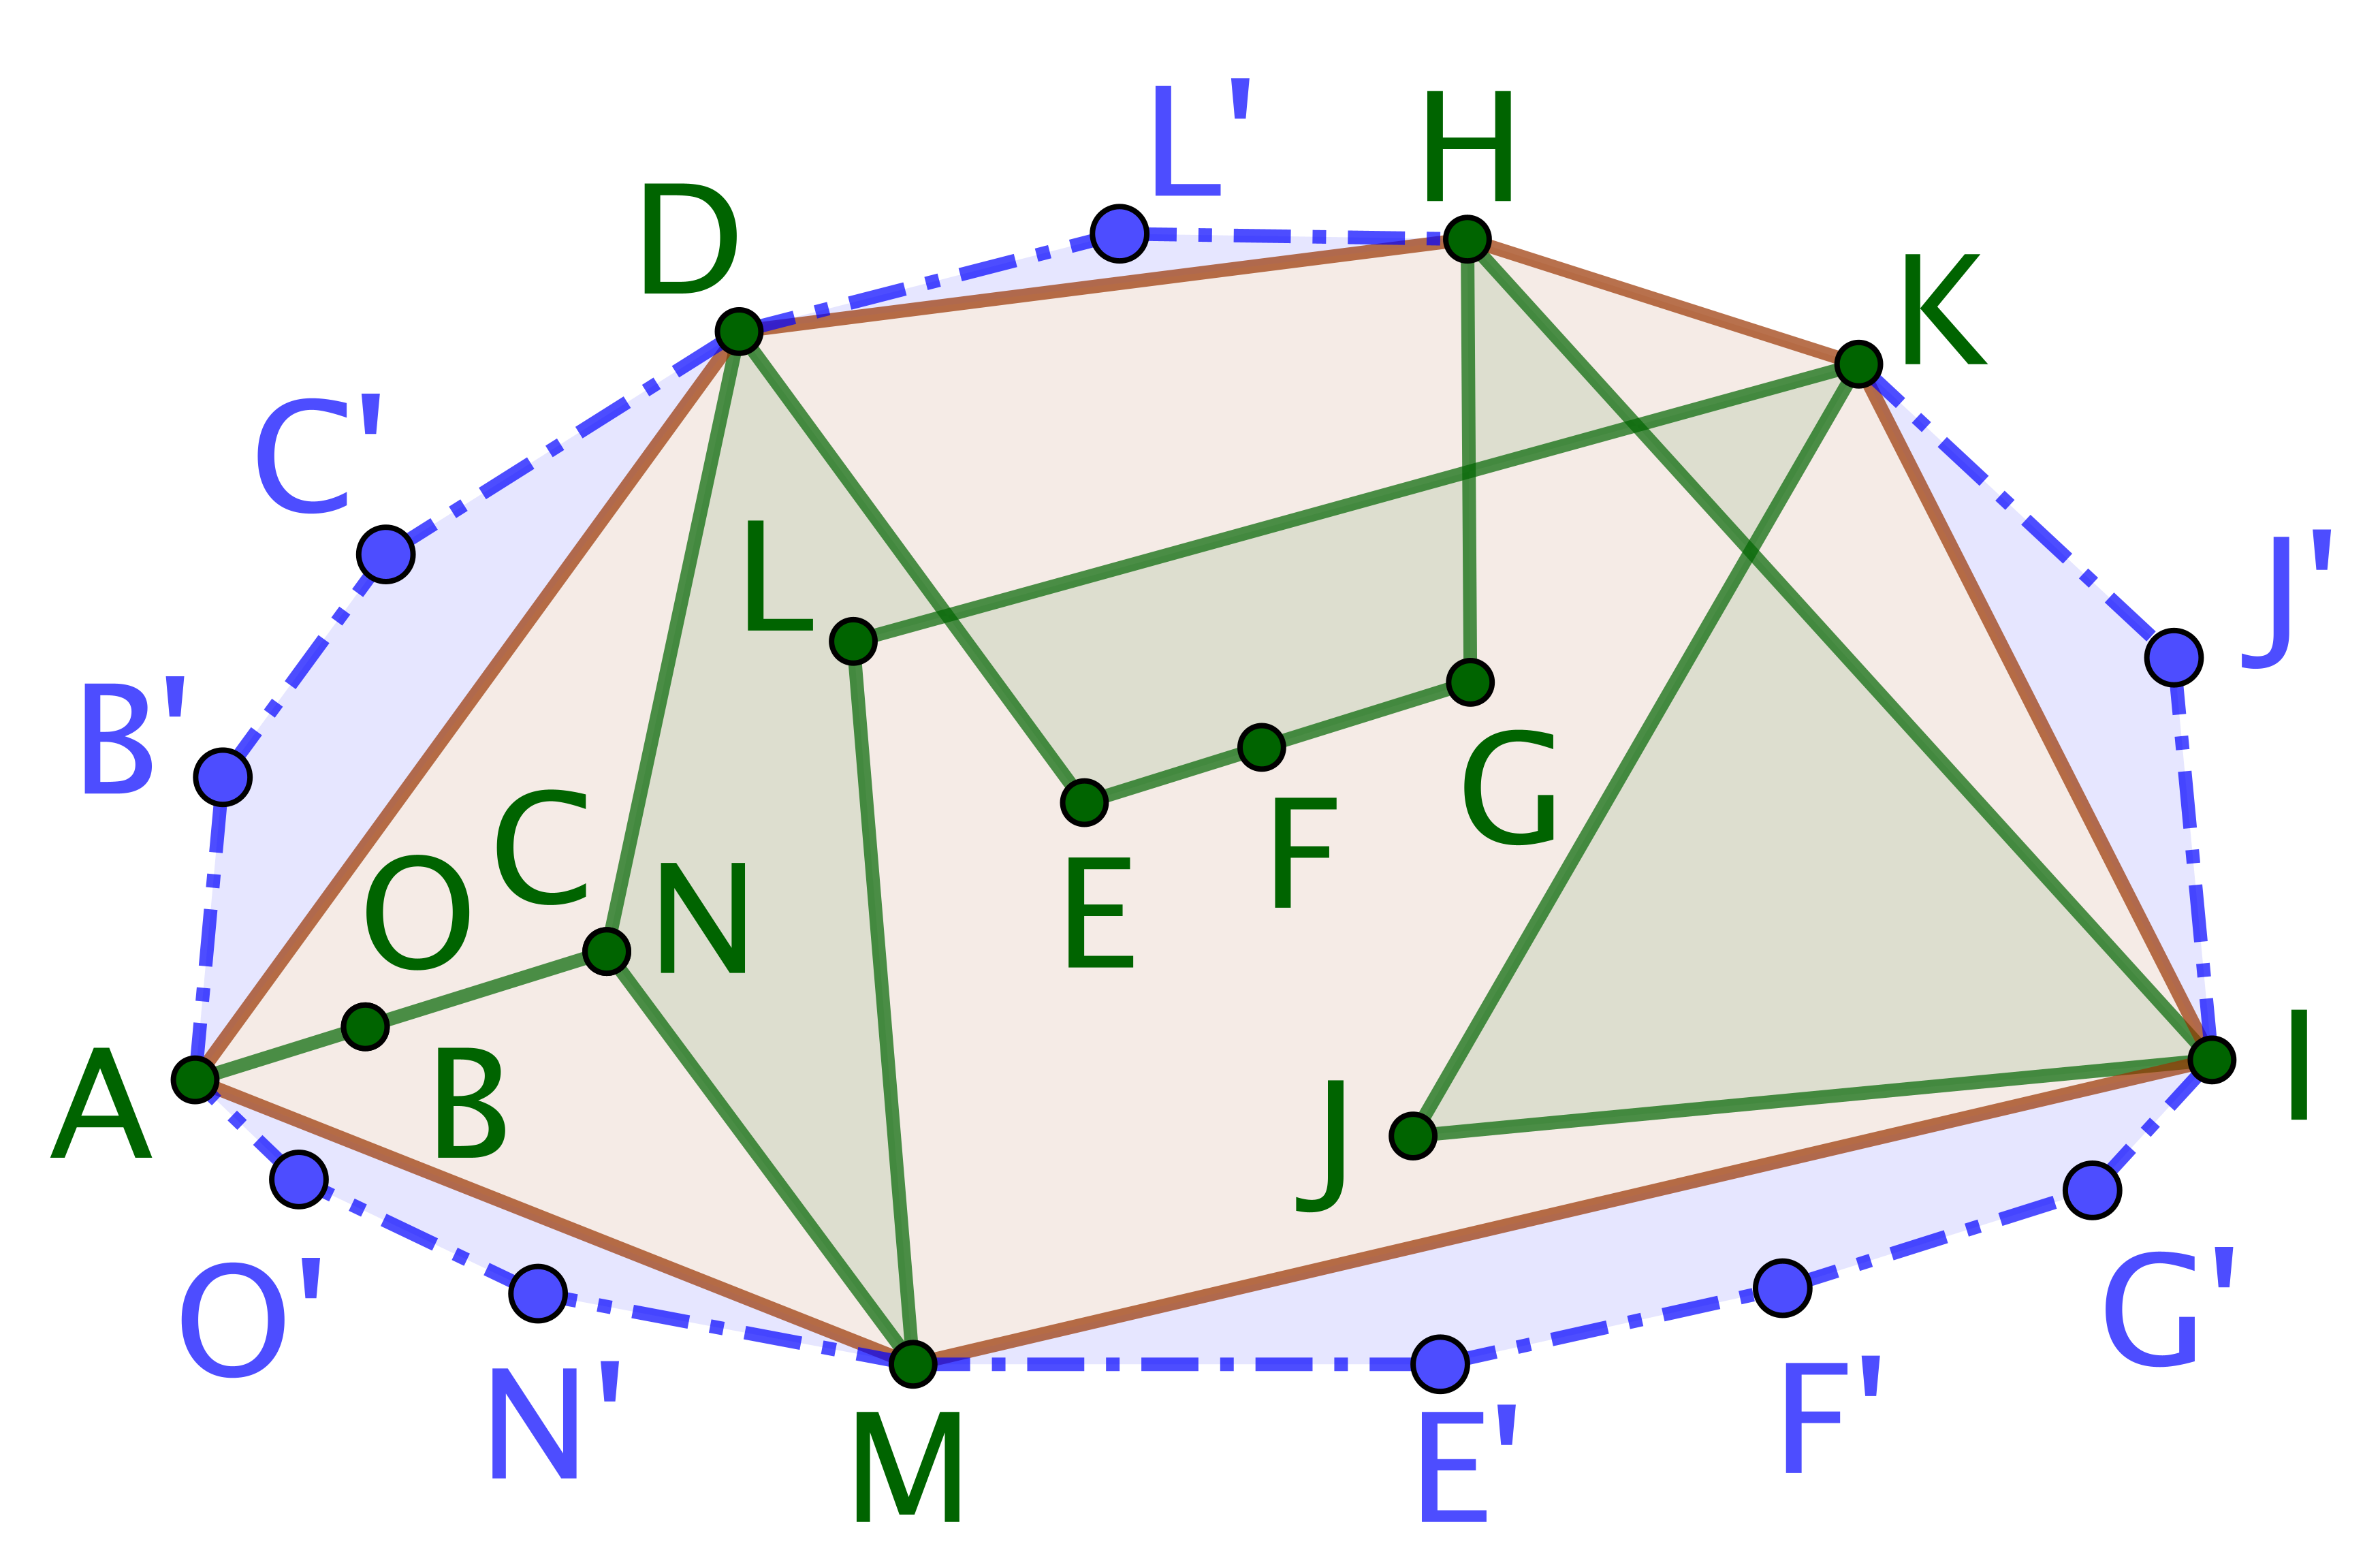
\includegraphics[scale=.45]{content/polygon/sol-must-be/convex-hull-distortion.png}
	\end{center}

	\newpage % TEMPO

	Notons $m = n - s$ qui compte les sommets manquants, puis posons
	$\delta = \frac{\perim{\setproba{P}} - \perim{\setproba{E}}}{m}$.
	%
	\begin{enumerate}
		\item \label{add-vertex-start}
		Considérons $[AB]$ un côté quelconque de $\setproba{E}$.
		Les droites portées par les côtés \focus{autour} de $[AB]$ \focus{dessinent} une région contenant toujours un triangle $ABC$ dont l'intérieur est à l'extérieur
		\footnote{
			C'est ce que l'on appelle de la \focus{low poetry},.
		}
		de $\setproba{E}$ comme dans les deux cas ci-dessous.
		%
		\begin{multicols}{2}
			\centering

			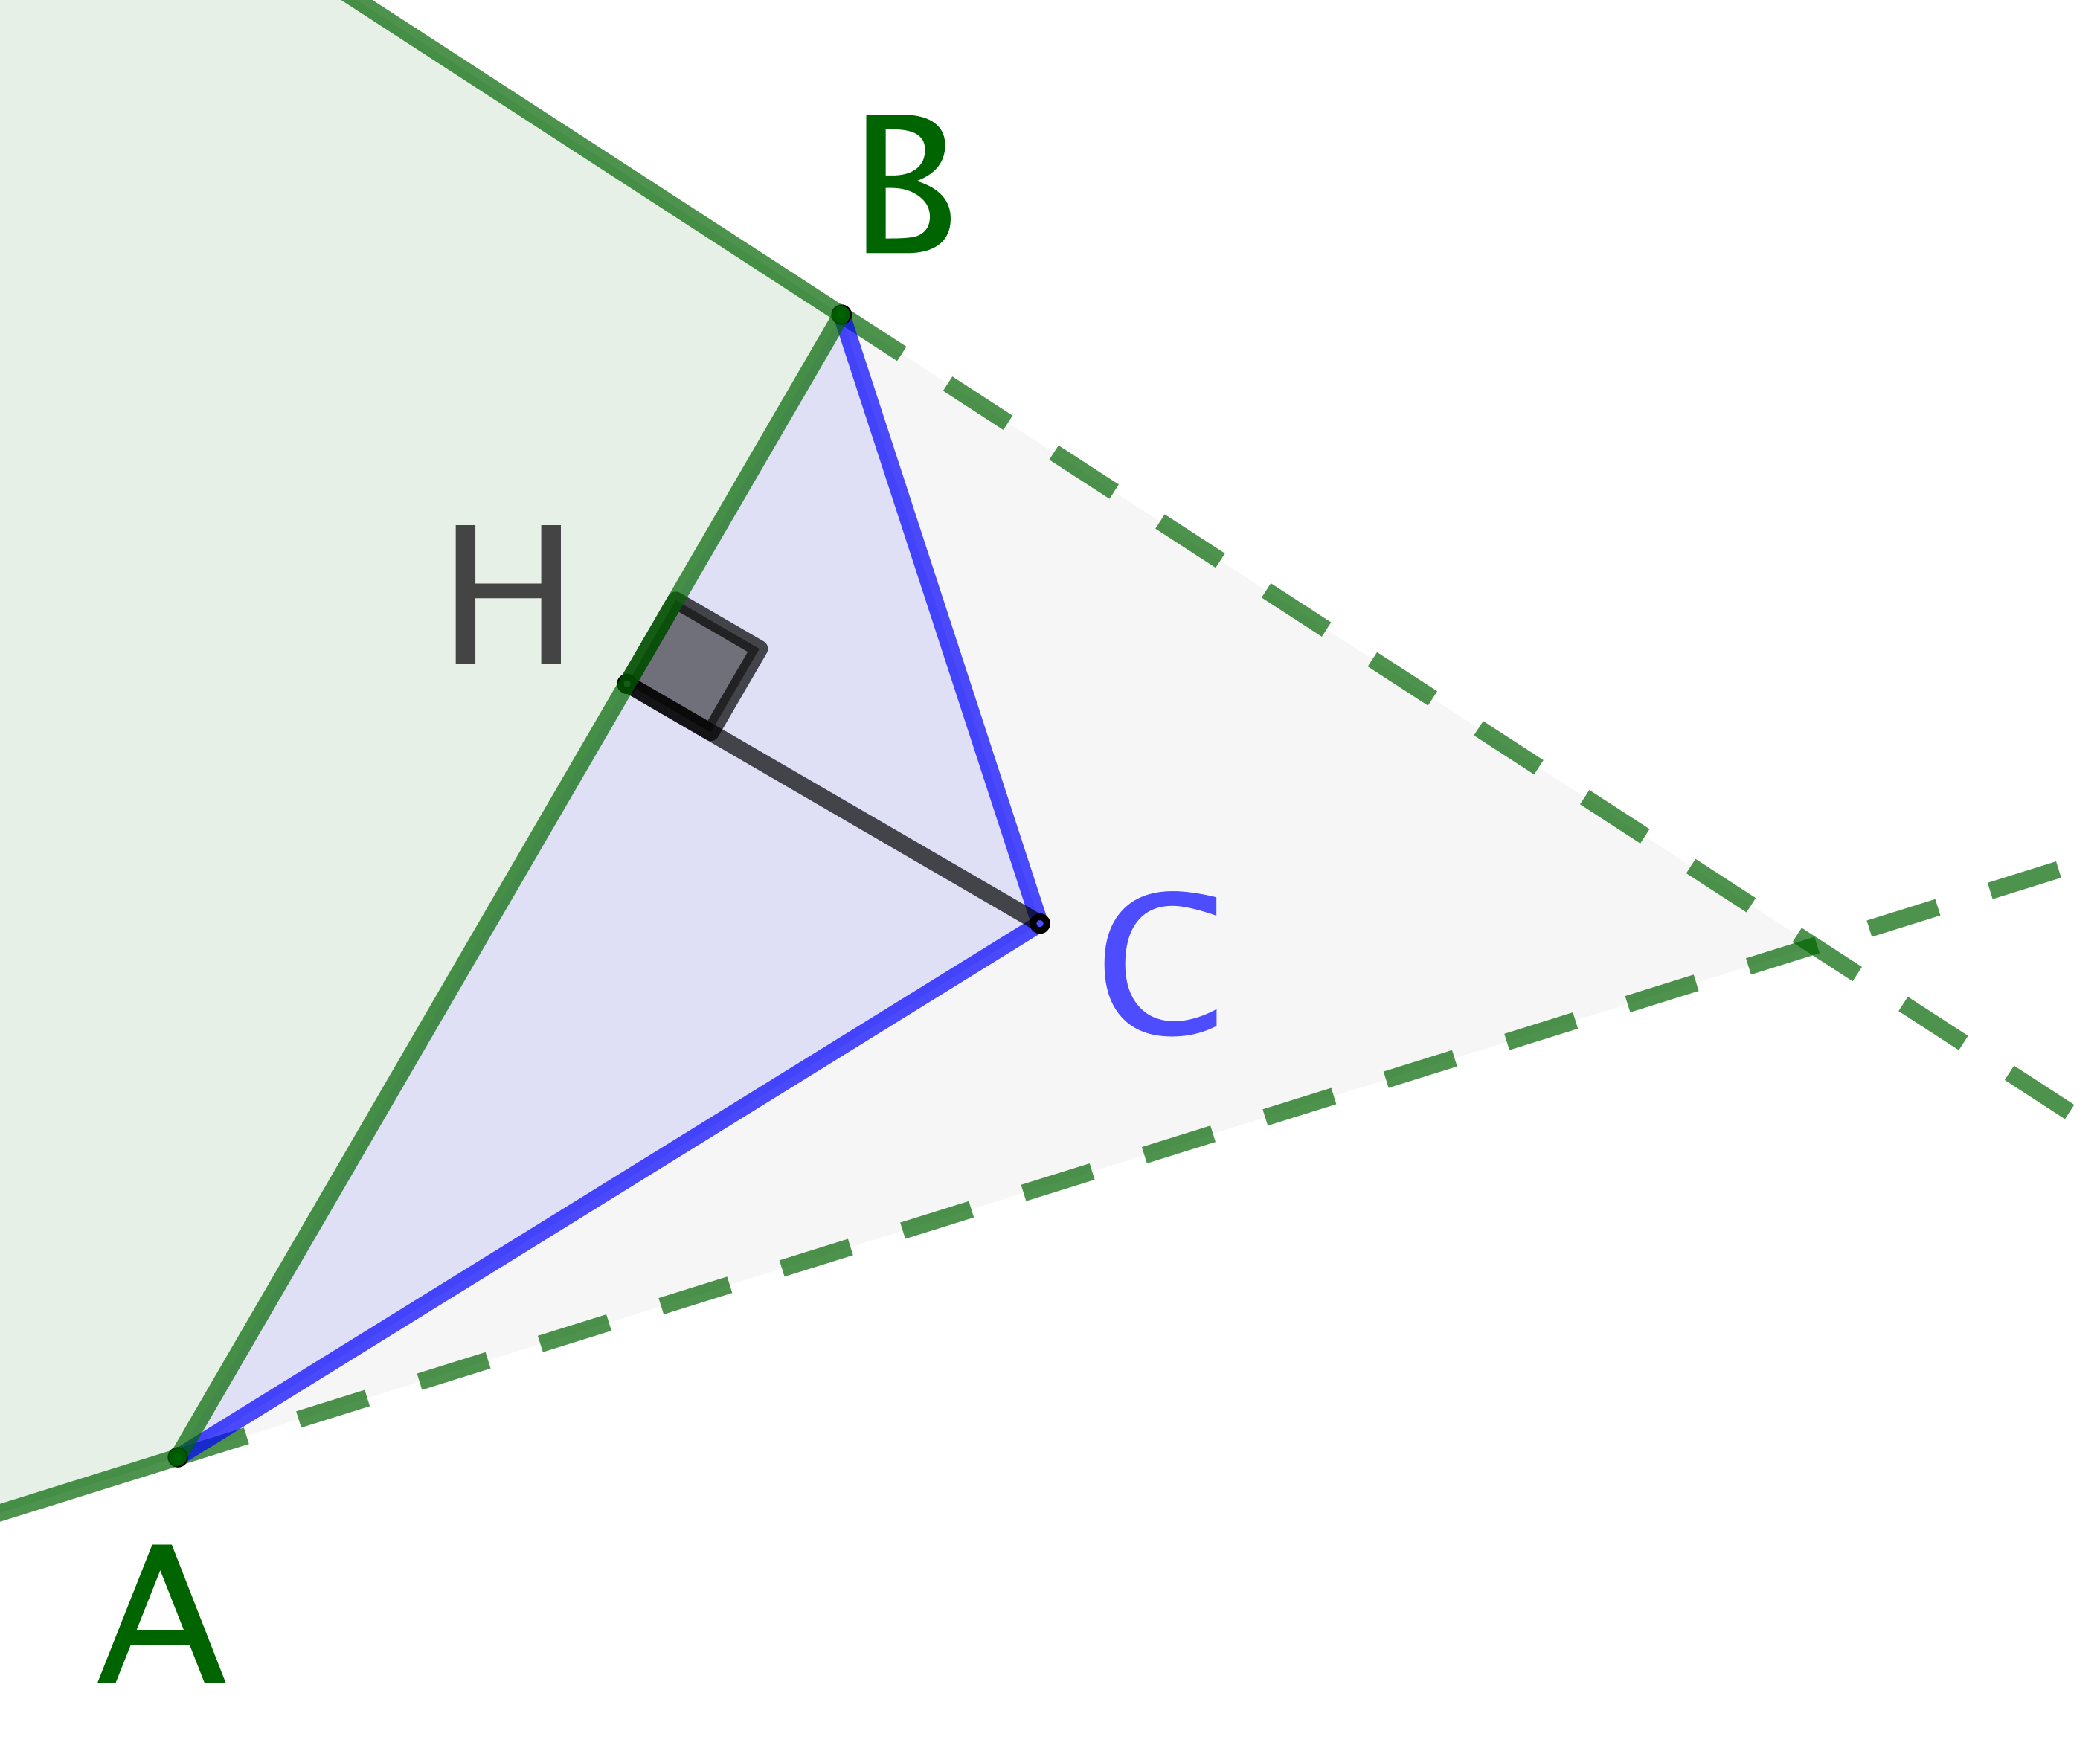
\includegraphics[scale=.35]{content/polygon/sol-must-be/add-vertex-1.png}

			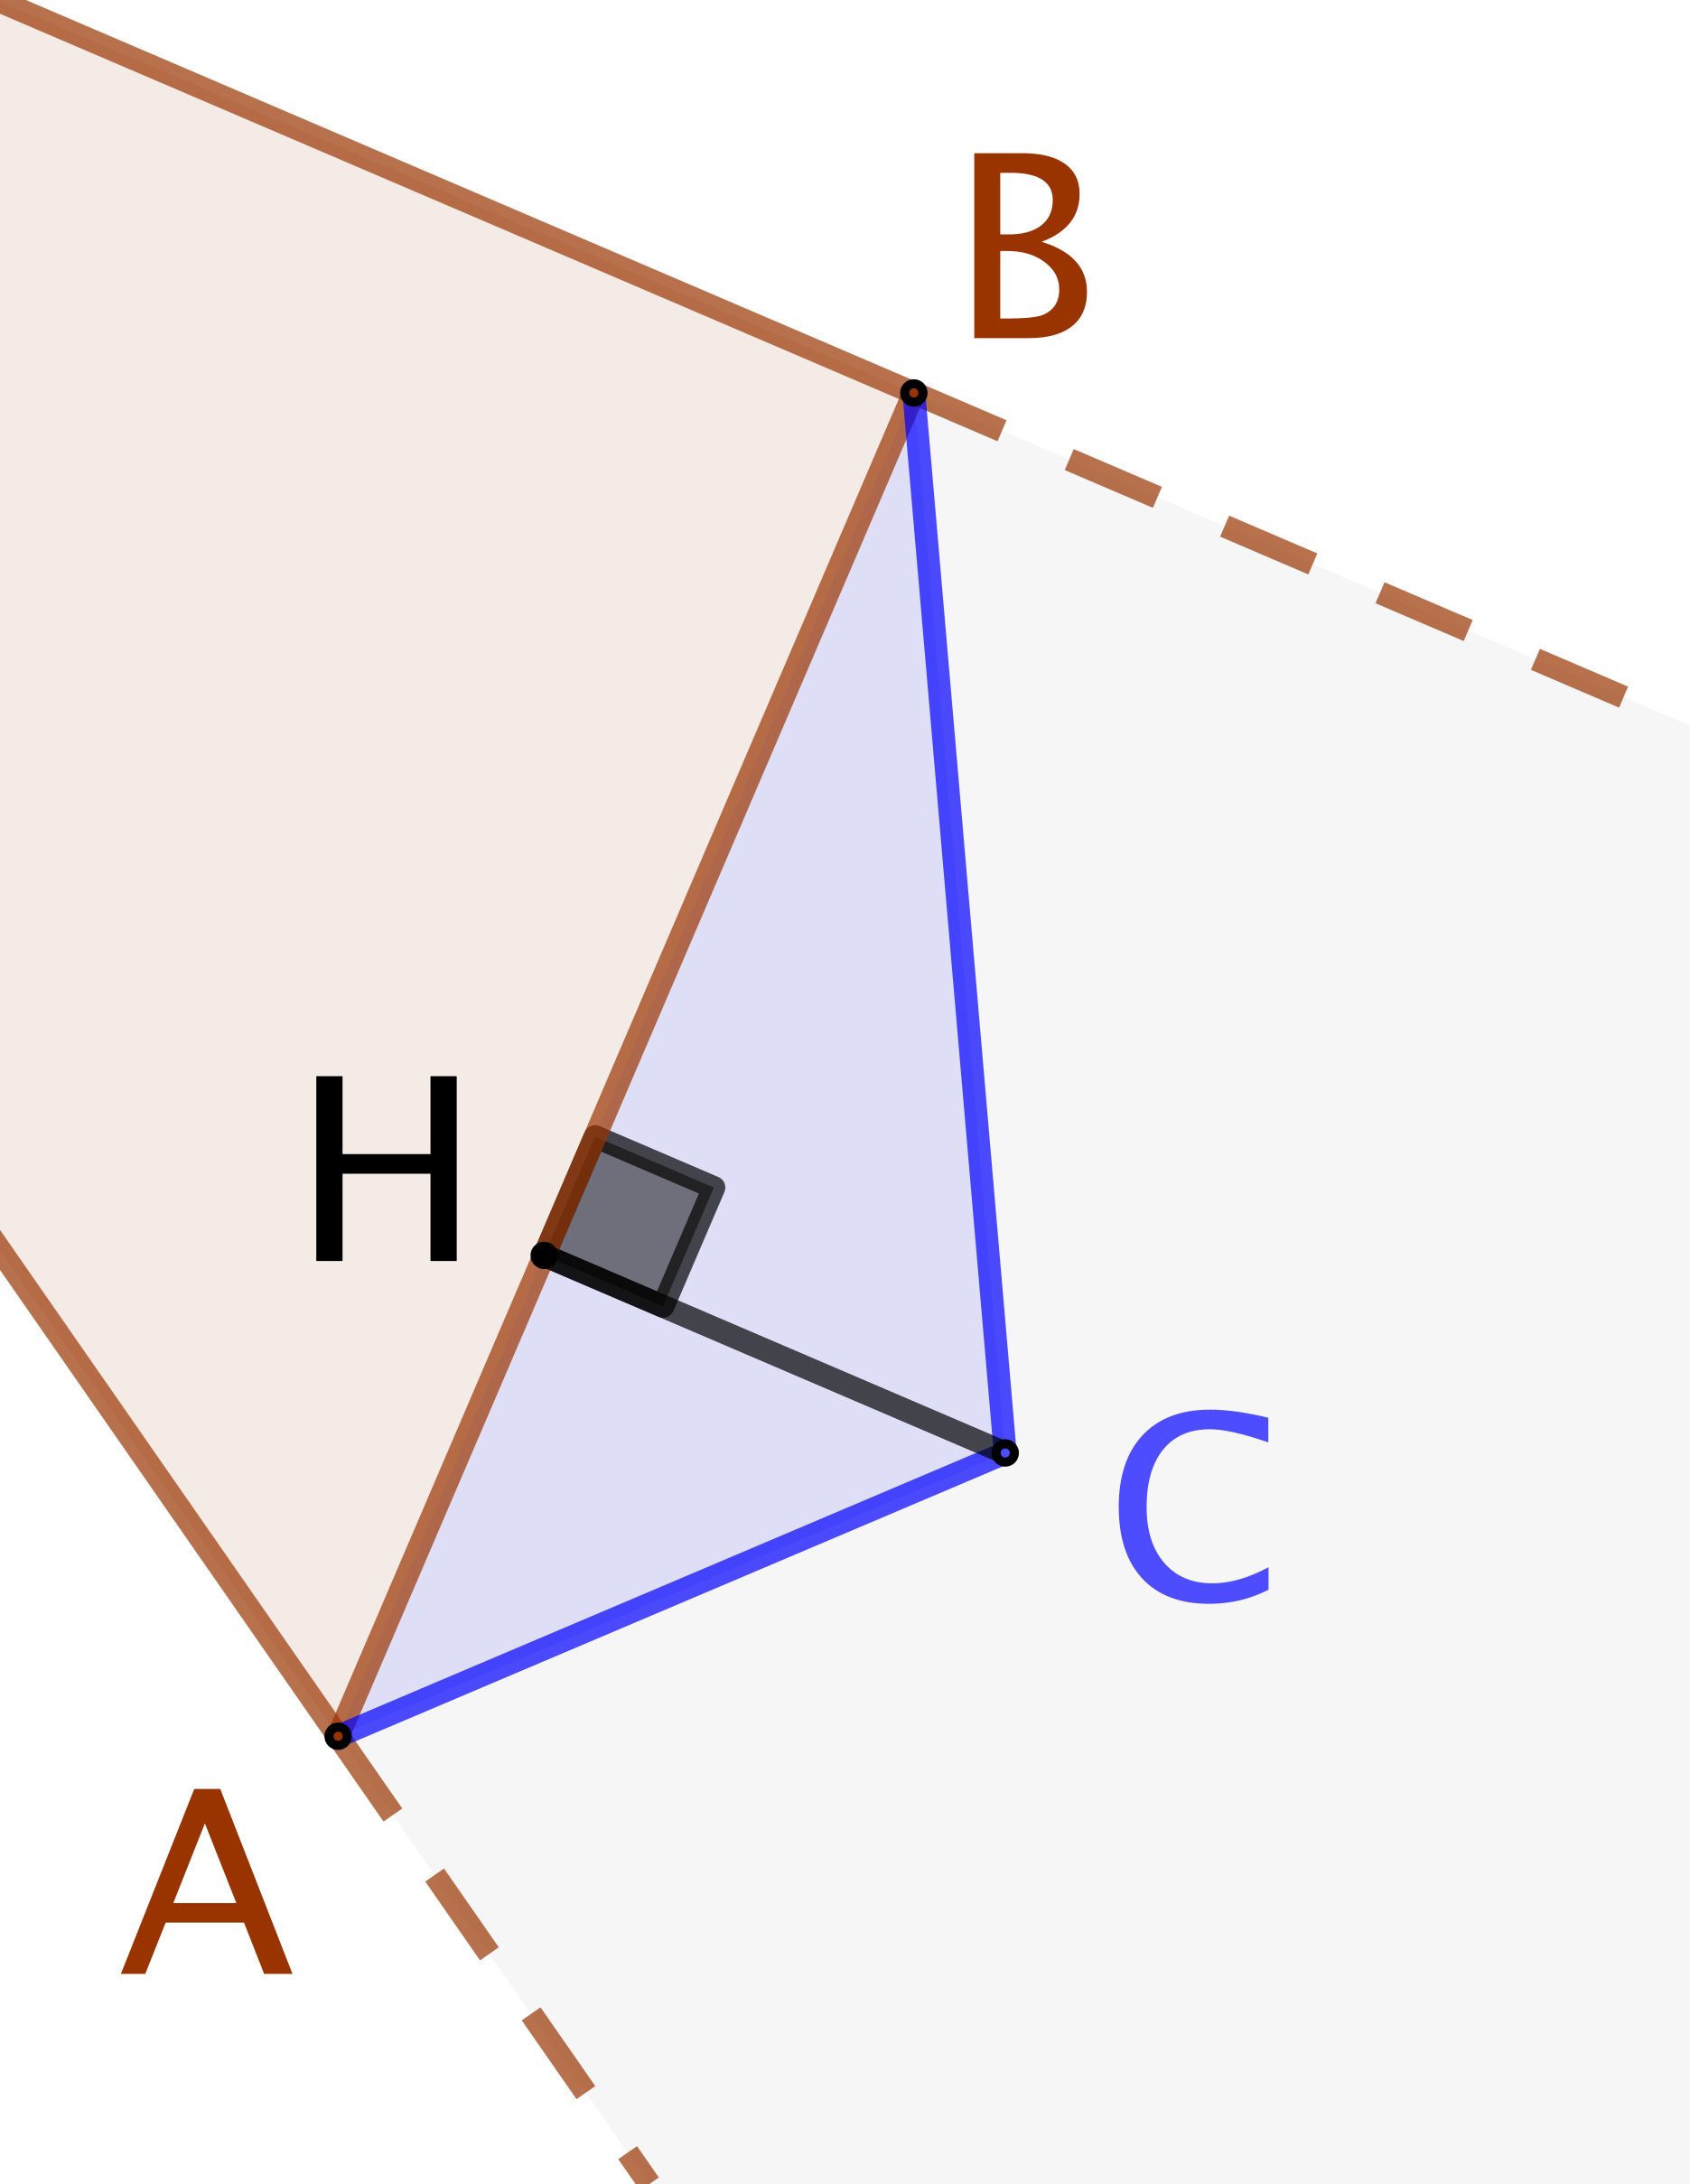
\includegraphics[scale=.35]{content/polygon/sol-must-be/add-vertex-2.png}
		\end{multicols}

		\item Clairement, le polygone $\setproba{E}_+$ obtenu à partir de $\setproba{E}$ en remplaçant le côté $[AB]$ par les côtés $[AC]$ et $[CB]$ est un convexe avec un sommet de plus que $\setproba{E}$.

		\item \label{add-vertex-end}
		Comme $HC$ peut être rendu aussi proche de $0$ que souhaité, il est aisé de voir que l'nous pouvons choisir cette distance de sorte que $AC + BC < AB + \delta$.
		Dès lors, le périmètre de $\setproba{E}_+$ augmente inférieurement strictement à $\delta$ relativement à $\setproba{E}$.

		\item En répétant $(m-1)$ fois les étapes \ref{add-vertex-start} à \ref{add-vertex-end}, nous obtenons un \ngone\ convexe $\setproba{C}$ tel que
		$\area{\setproba{C}} > \area{\setproba{P}}$
		et
		$\perim{\setproba{C}} < \perim{\setproba{E}} + m \delta = \perim{\setproba{P}}$.
	\end{enumerate}
	
	\null\vspace{-6ex}
\end{proof}


% ----------------------- %


\begin{fact} \label{must-be-equi}
	Si un \ngone\ convexe $\setproba{P}$ n'est pas équilatéral,
	alors nous pouvons construire un \ngone\ convexe $\primeit{\setproba{P}}$ tel que
	$\perim{\primeit{\setproba{P}}} = \perim{\setproba{P}}$
	et
	$\area{\primeit{\setproba{P}}} > \area{\setproba{P}}$.
\end{fact}


\begin{proof}
	Considérons un \ngone\ convexe non équilatéral $\setproba{P}$.
	%
	Dans ce cas, $\setproba{P}$ admet un triplet de sommets consécutifs $A$, $B$ et $C$ tels que $AB \neq BC$
	(sinon, on obtiendrait de proche en proche l'équilatéralité).
	La construction vue dans la preuve du fait \ref{tri-one-side-fixed} nous donne la solution: voir les deux dessins ci-après dans lesquels $(AC) \parallel (BB^{\,\prime})$.
	Pour le 2\ieme\ cas, il n'est pas possible d'utiliser le triangle $AB^{\,\prime}C$ isocèle en $B^{\,\prime}$ car $(B^{\,\prime}C)$ porte le côté de $\setproba{P}$ de sommet $C$ juste après $[BC]$, mais ce problème se contourne en considérant un point $B^{\,\prime\prime}$ du segment ouvert $]BB^{\,\prime}[$ (si besoin, se reporter au 2\ieme\ dessin de la preuve du fait \ref{tri-one-side-fixed}).
	%
	\begin{multicols}{2}
		\centering

		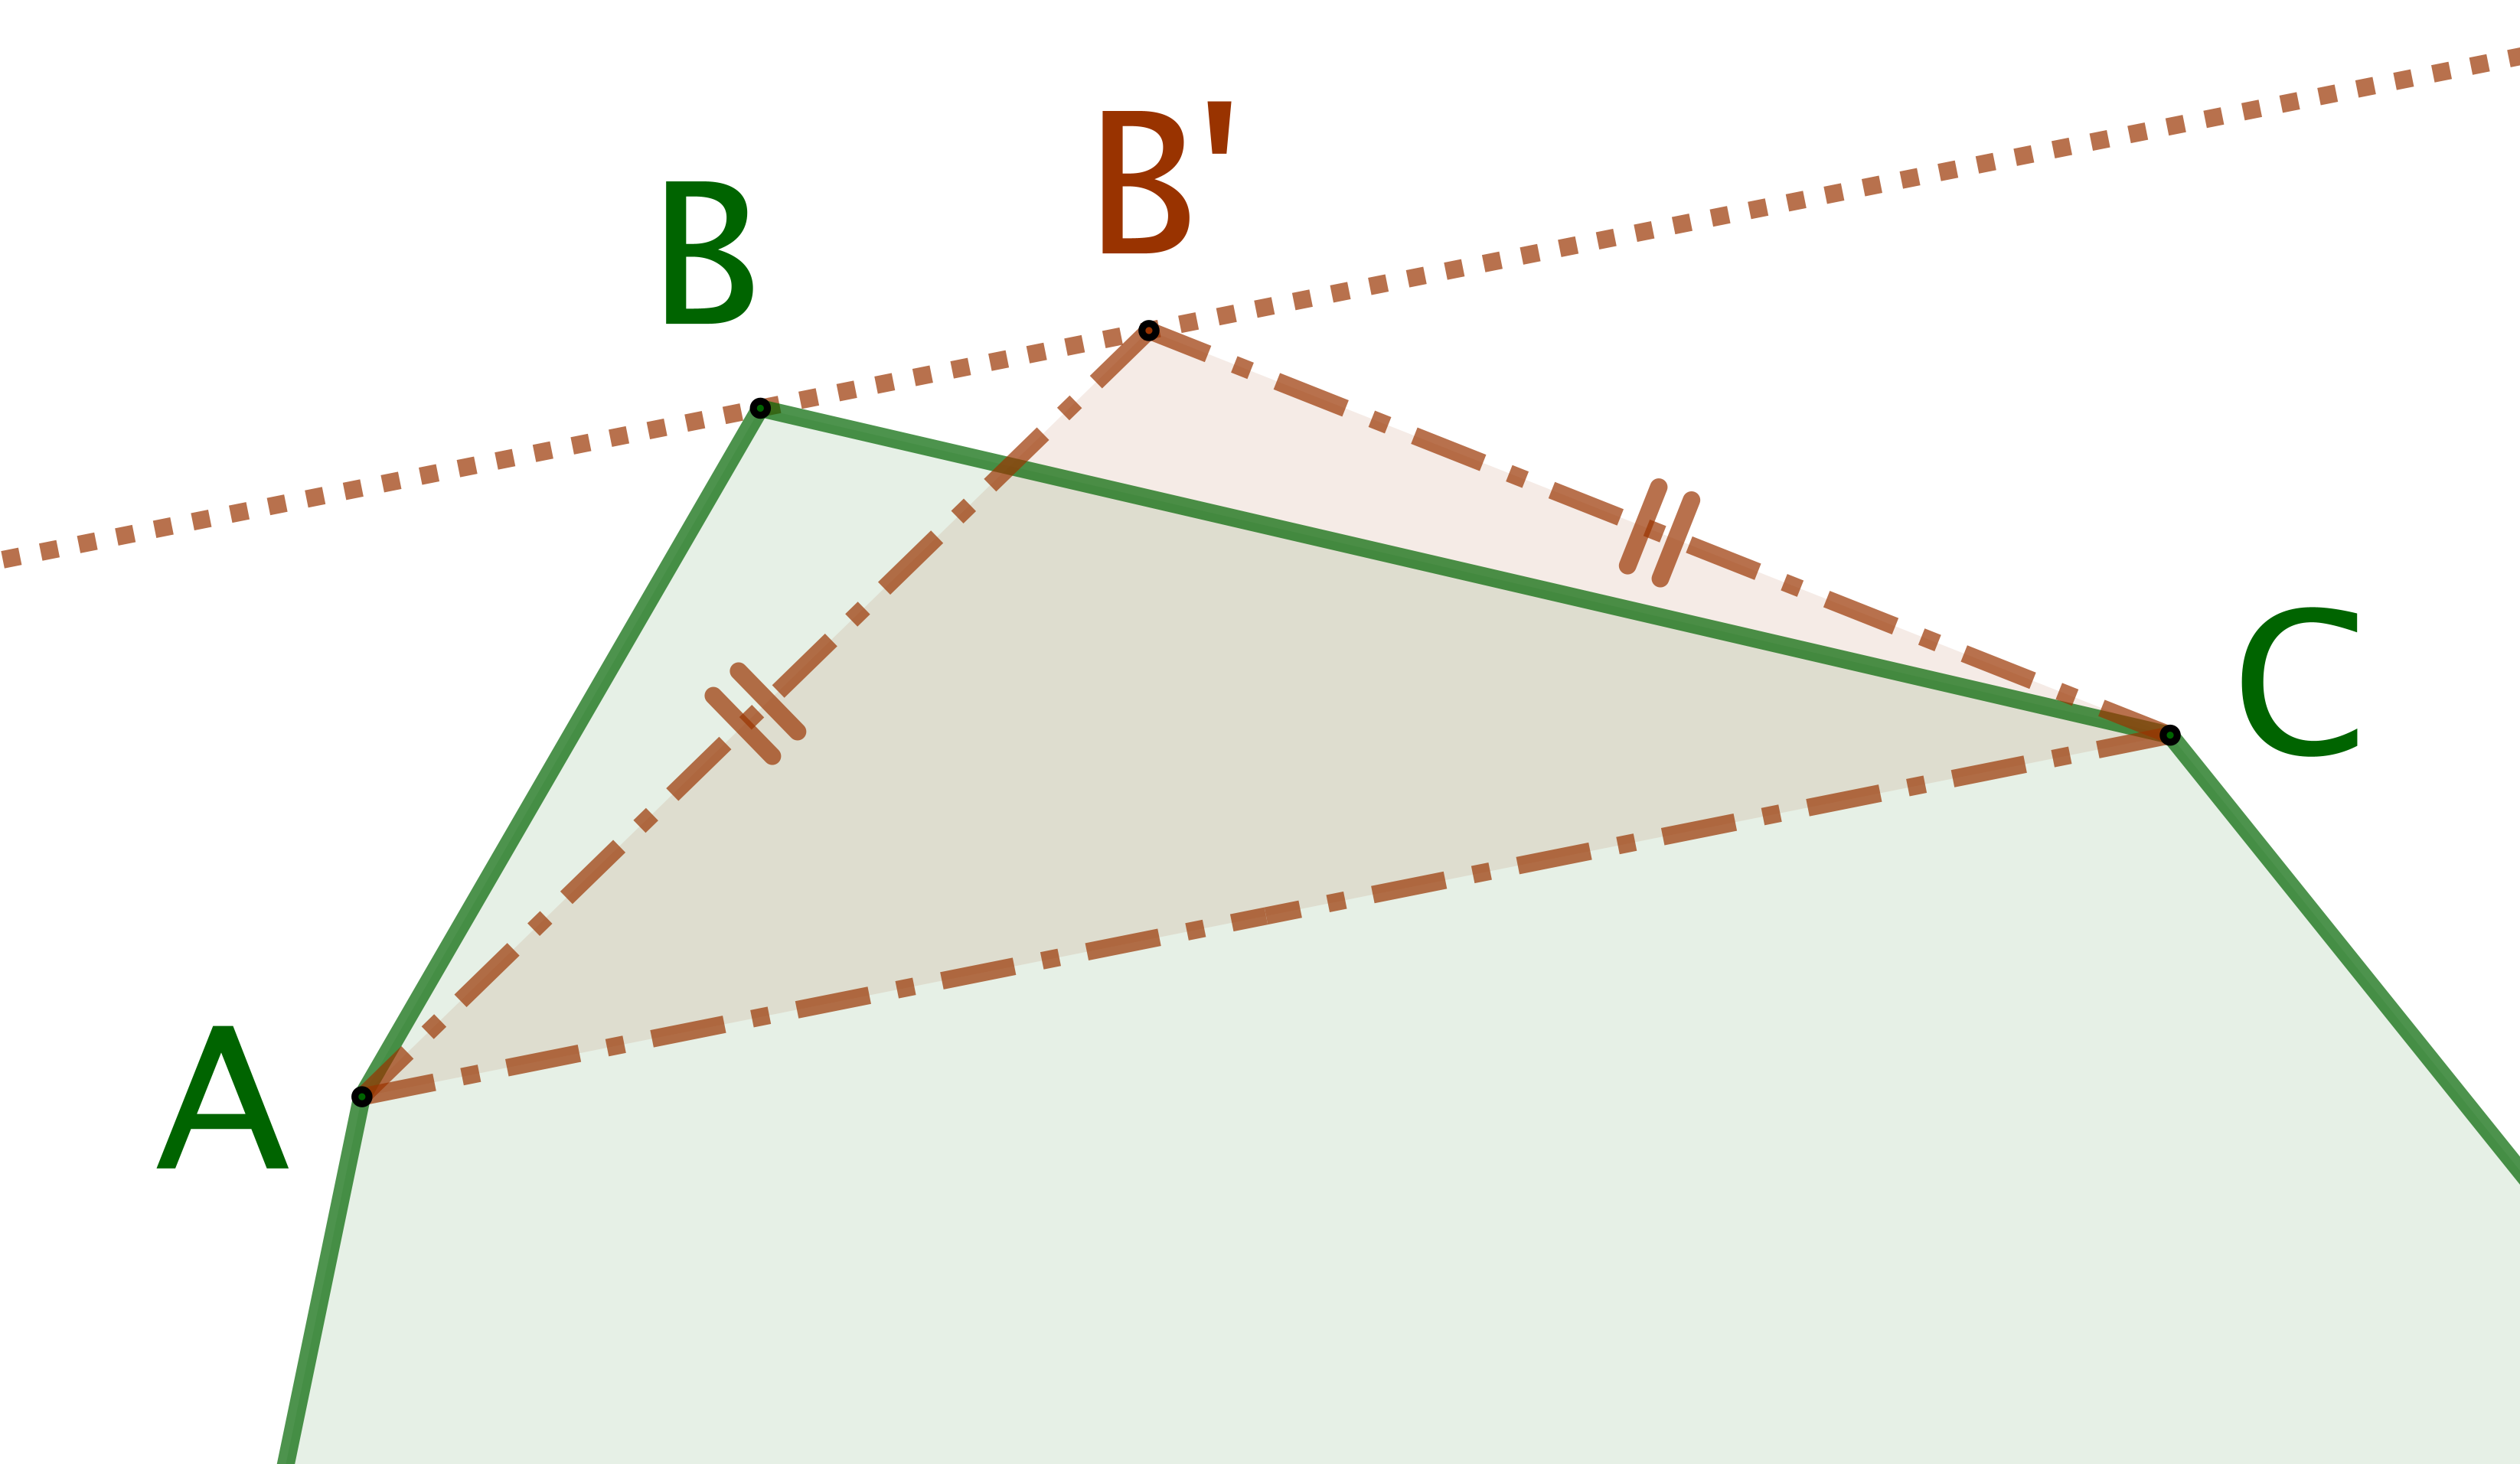
\includegraphics[scale=.4]{content/polygon/sol-must-be/not-iso-OK.png}

		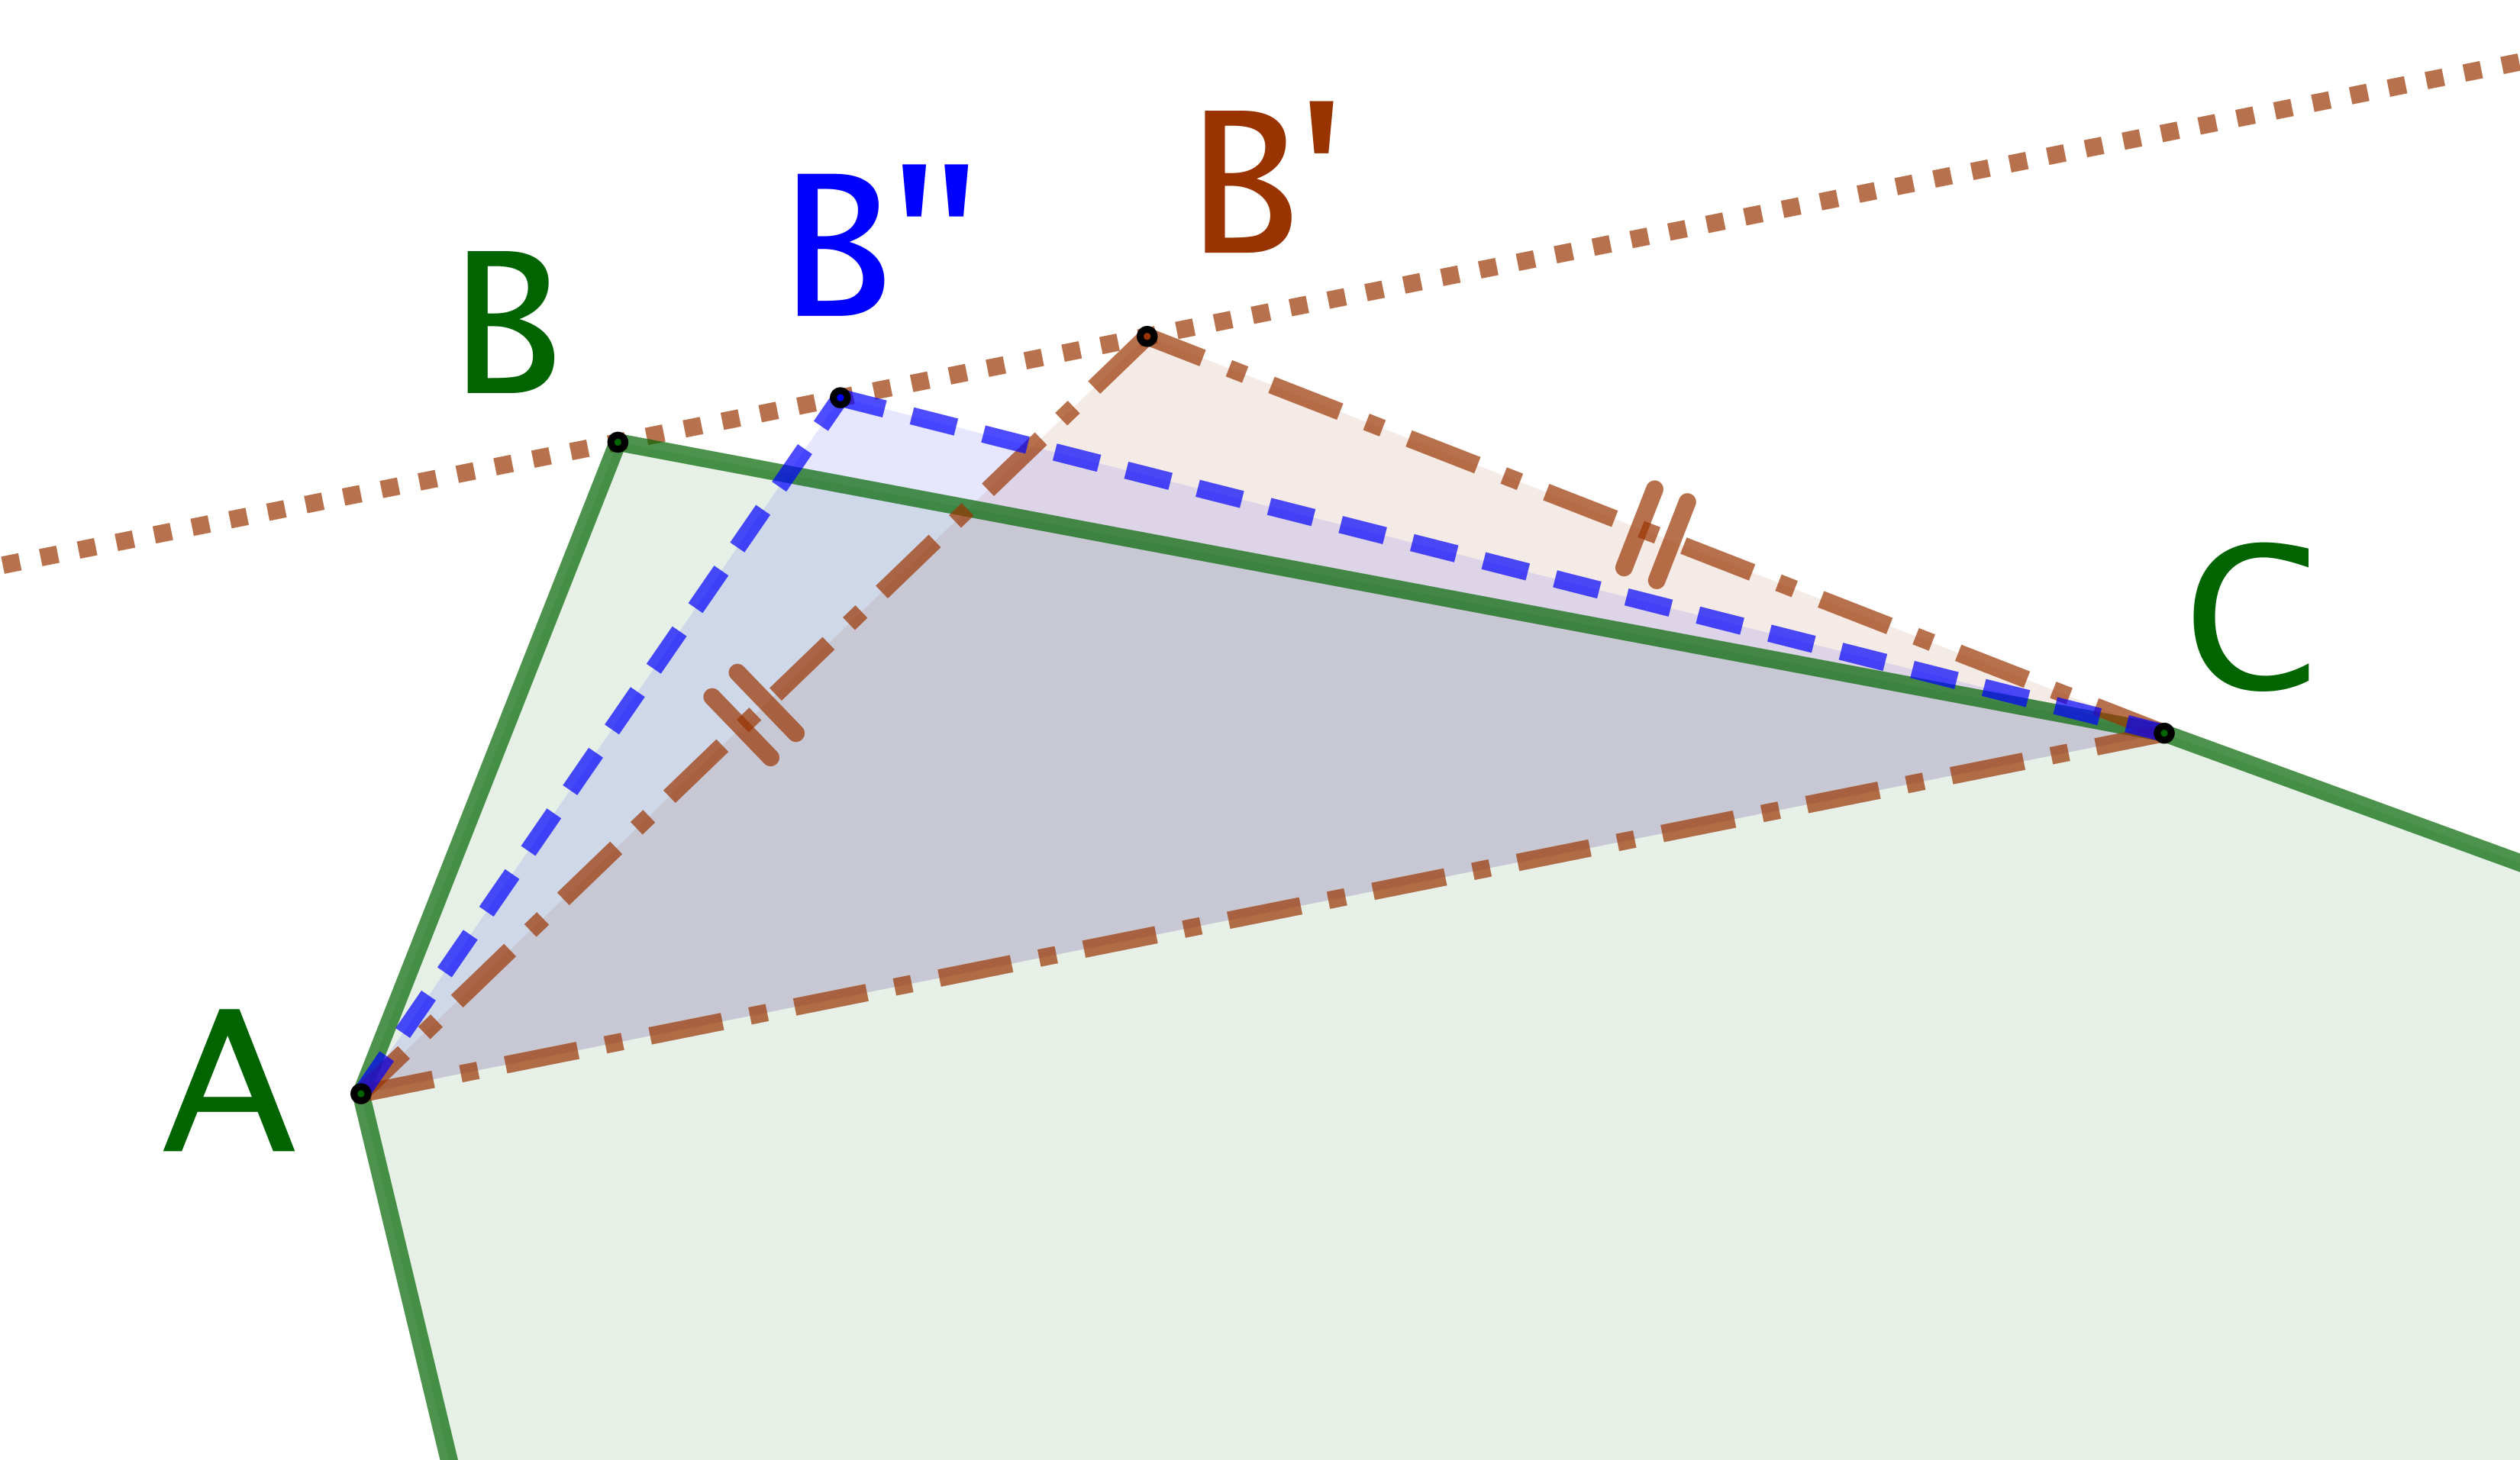
\includegraphics[scale=.4]{content/polygon/sol-must-be/not-iso-KO.png}
	\end{multicols}

	Dans chaque cas, nous avons construit un \ngone\ convexe $\dbleprimeit{\setproba{P}}$ tel que
	$\perim{\dbleprimeit{\setproba{P}}} < \perim{\setproba{P}}$
	et
	$\area{\dbleprimeit{\setproba{P}}} = \area{\setproba{P}}$.
	Une homothétie de rapport $r > 1$, où $r = \frac{ \perim{\setproba{P}} }{ \perim{\setproba{E}} }$, donne un \ngone\ convexe $\primeit{\setproba{P}}$ vérifiant
	$\perim{\primeit{\setproba{P}}} = \perim{\setproba{P}}$
	et
	$\area{\primeit{\setproba{P}}} > \area{\setproba{P}}$.
\end{proof}


\begin{remark}
	Le fait précédent ne permet pas de toujours se ramener au cas d'un \nequi\ convexe. Il nous dit juste que si un \ngone\ convexe maximise son aire à périmètre fixé, alors il devra être, a minima, un \nequi. La nuance est importante, et une similaire existe pour la conclusion du fait suivant.
\end{remark}


% ----------------------- %


\begin{fact} \label{must-be-iso}
	Si un \nequi\ convexe $\setproba{P}$ n'est pas équiangle,
	alors il existe un \ngone\ convexe $\primeit{\setproba{P}}$ tel que
	$\perim{\primeit{\setproba{P}}} = \perim{\setproba{P}}$
	et
	$\area{\primeit{\setproba{P}}} > \area{\setproba{P}}$.
\end{fact}


\begin{proof}
	Considérons un \nequi\ convexe non équiangle $\setproba{P}$.
	%
	Dans ce cas, $\setproba{P}$ admet un quadruplet de sommets consécutifs $A$, $B$, $C$ et $D$ tels que $\anglein{ABC} \neq \anglein{BCD}$
	(sinon, on obtiendrait de proche en proche l'équiangularité).
	Quitte à changer l'ordre de parcours des sommets de $\setproba{P}$, nous pouvons supposer $\anglein{ABC} > \anglein{BCD}$.
	%
	\begin{center}
		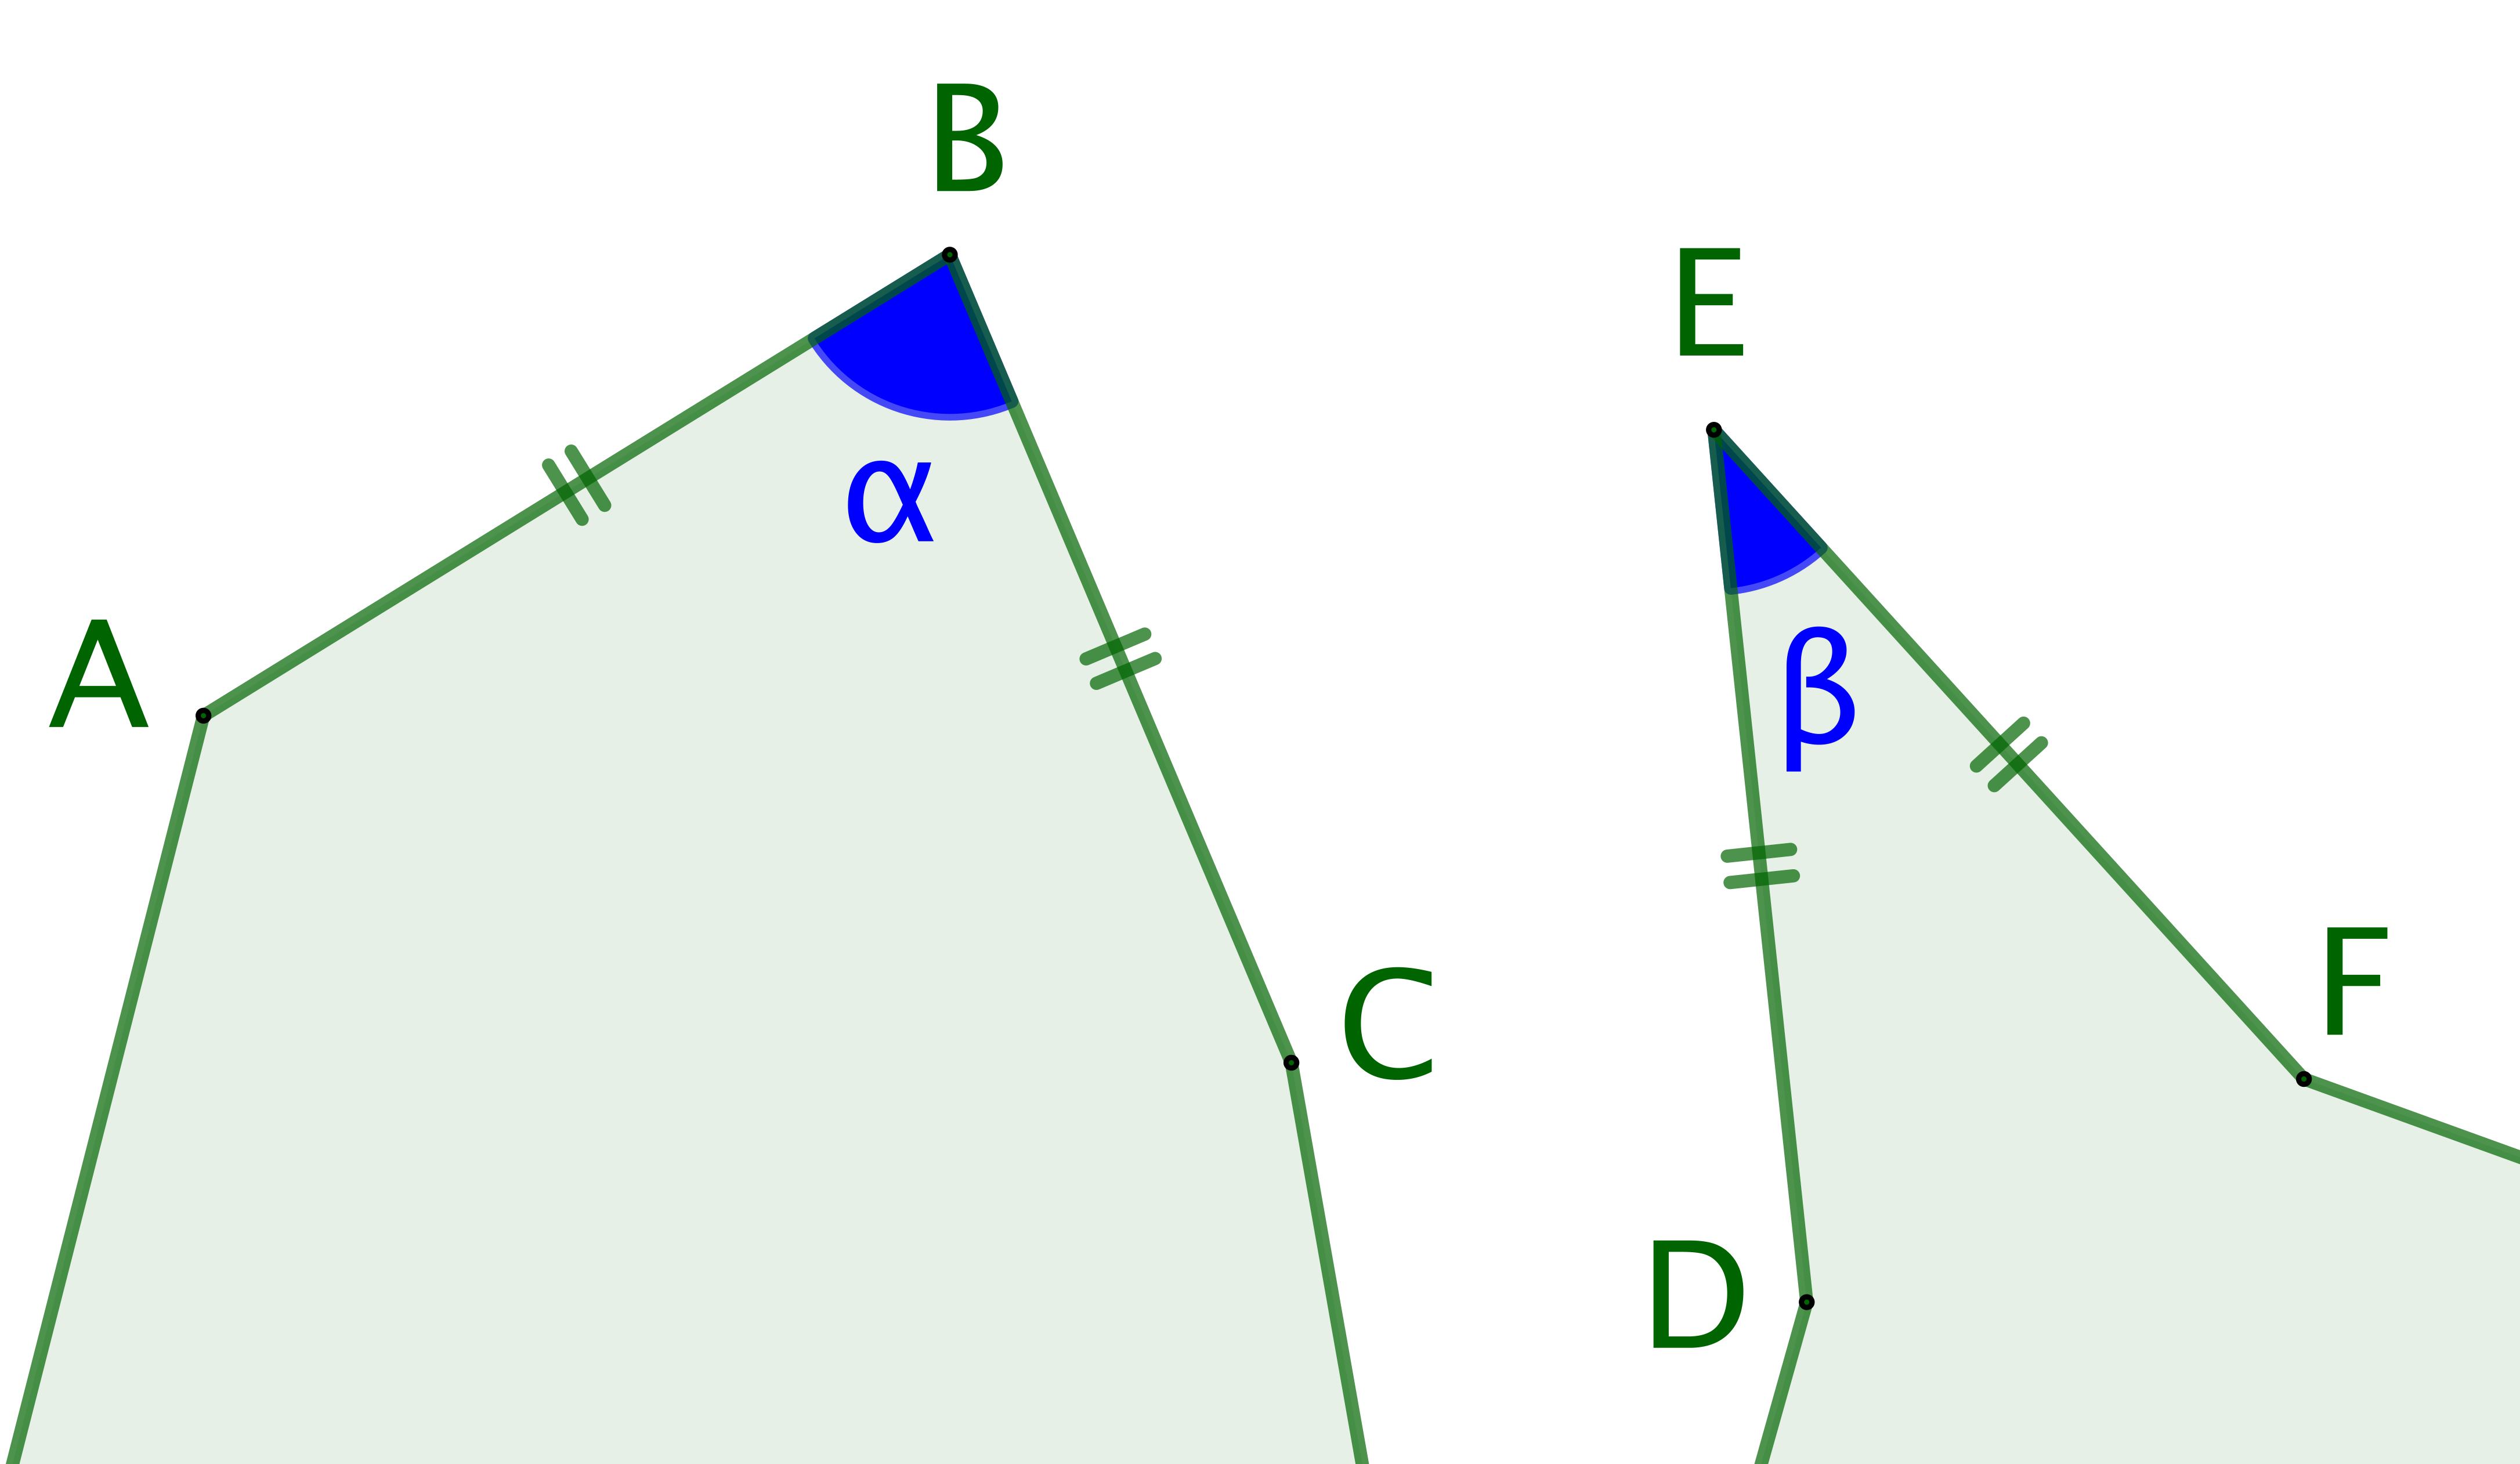
\includegraphics[scale=.4]{content/polygon/sol-must-be/2-eq-angles-start.png}
	\end{center}
	
	En déplaçant $B$ et $C$ dans la zone grise hachurée strictement entre les droites vertes en pointillés, nous garderons un \ngone\ convexe.
	%
	Concentrons-nous donc sur le quadrilatère $ABCD$, et posons $c = AB$ la longueur commune des côtés de $\setproba{P}$, ainsi que $d = AD$ que nous ne pouvons pas modifier.
	%
	Si nous fixons la valeur de $c$, notre situation possède juste un degré de liberté comme le montre la construction de $C$ ci-après qui utilise des cercles de rayon $c$ centrés en $A$ et $D$ fixes, et $B$ mobile.
	%
	\begin{center}
		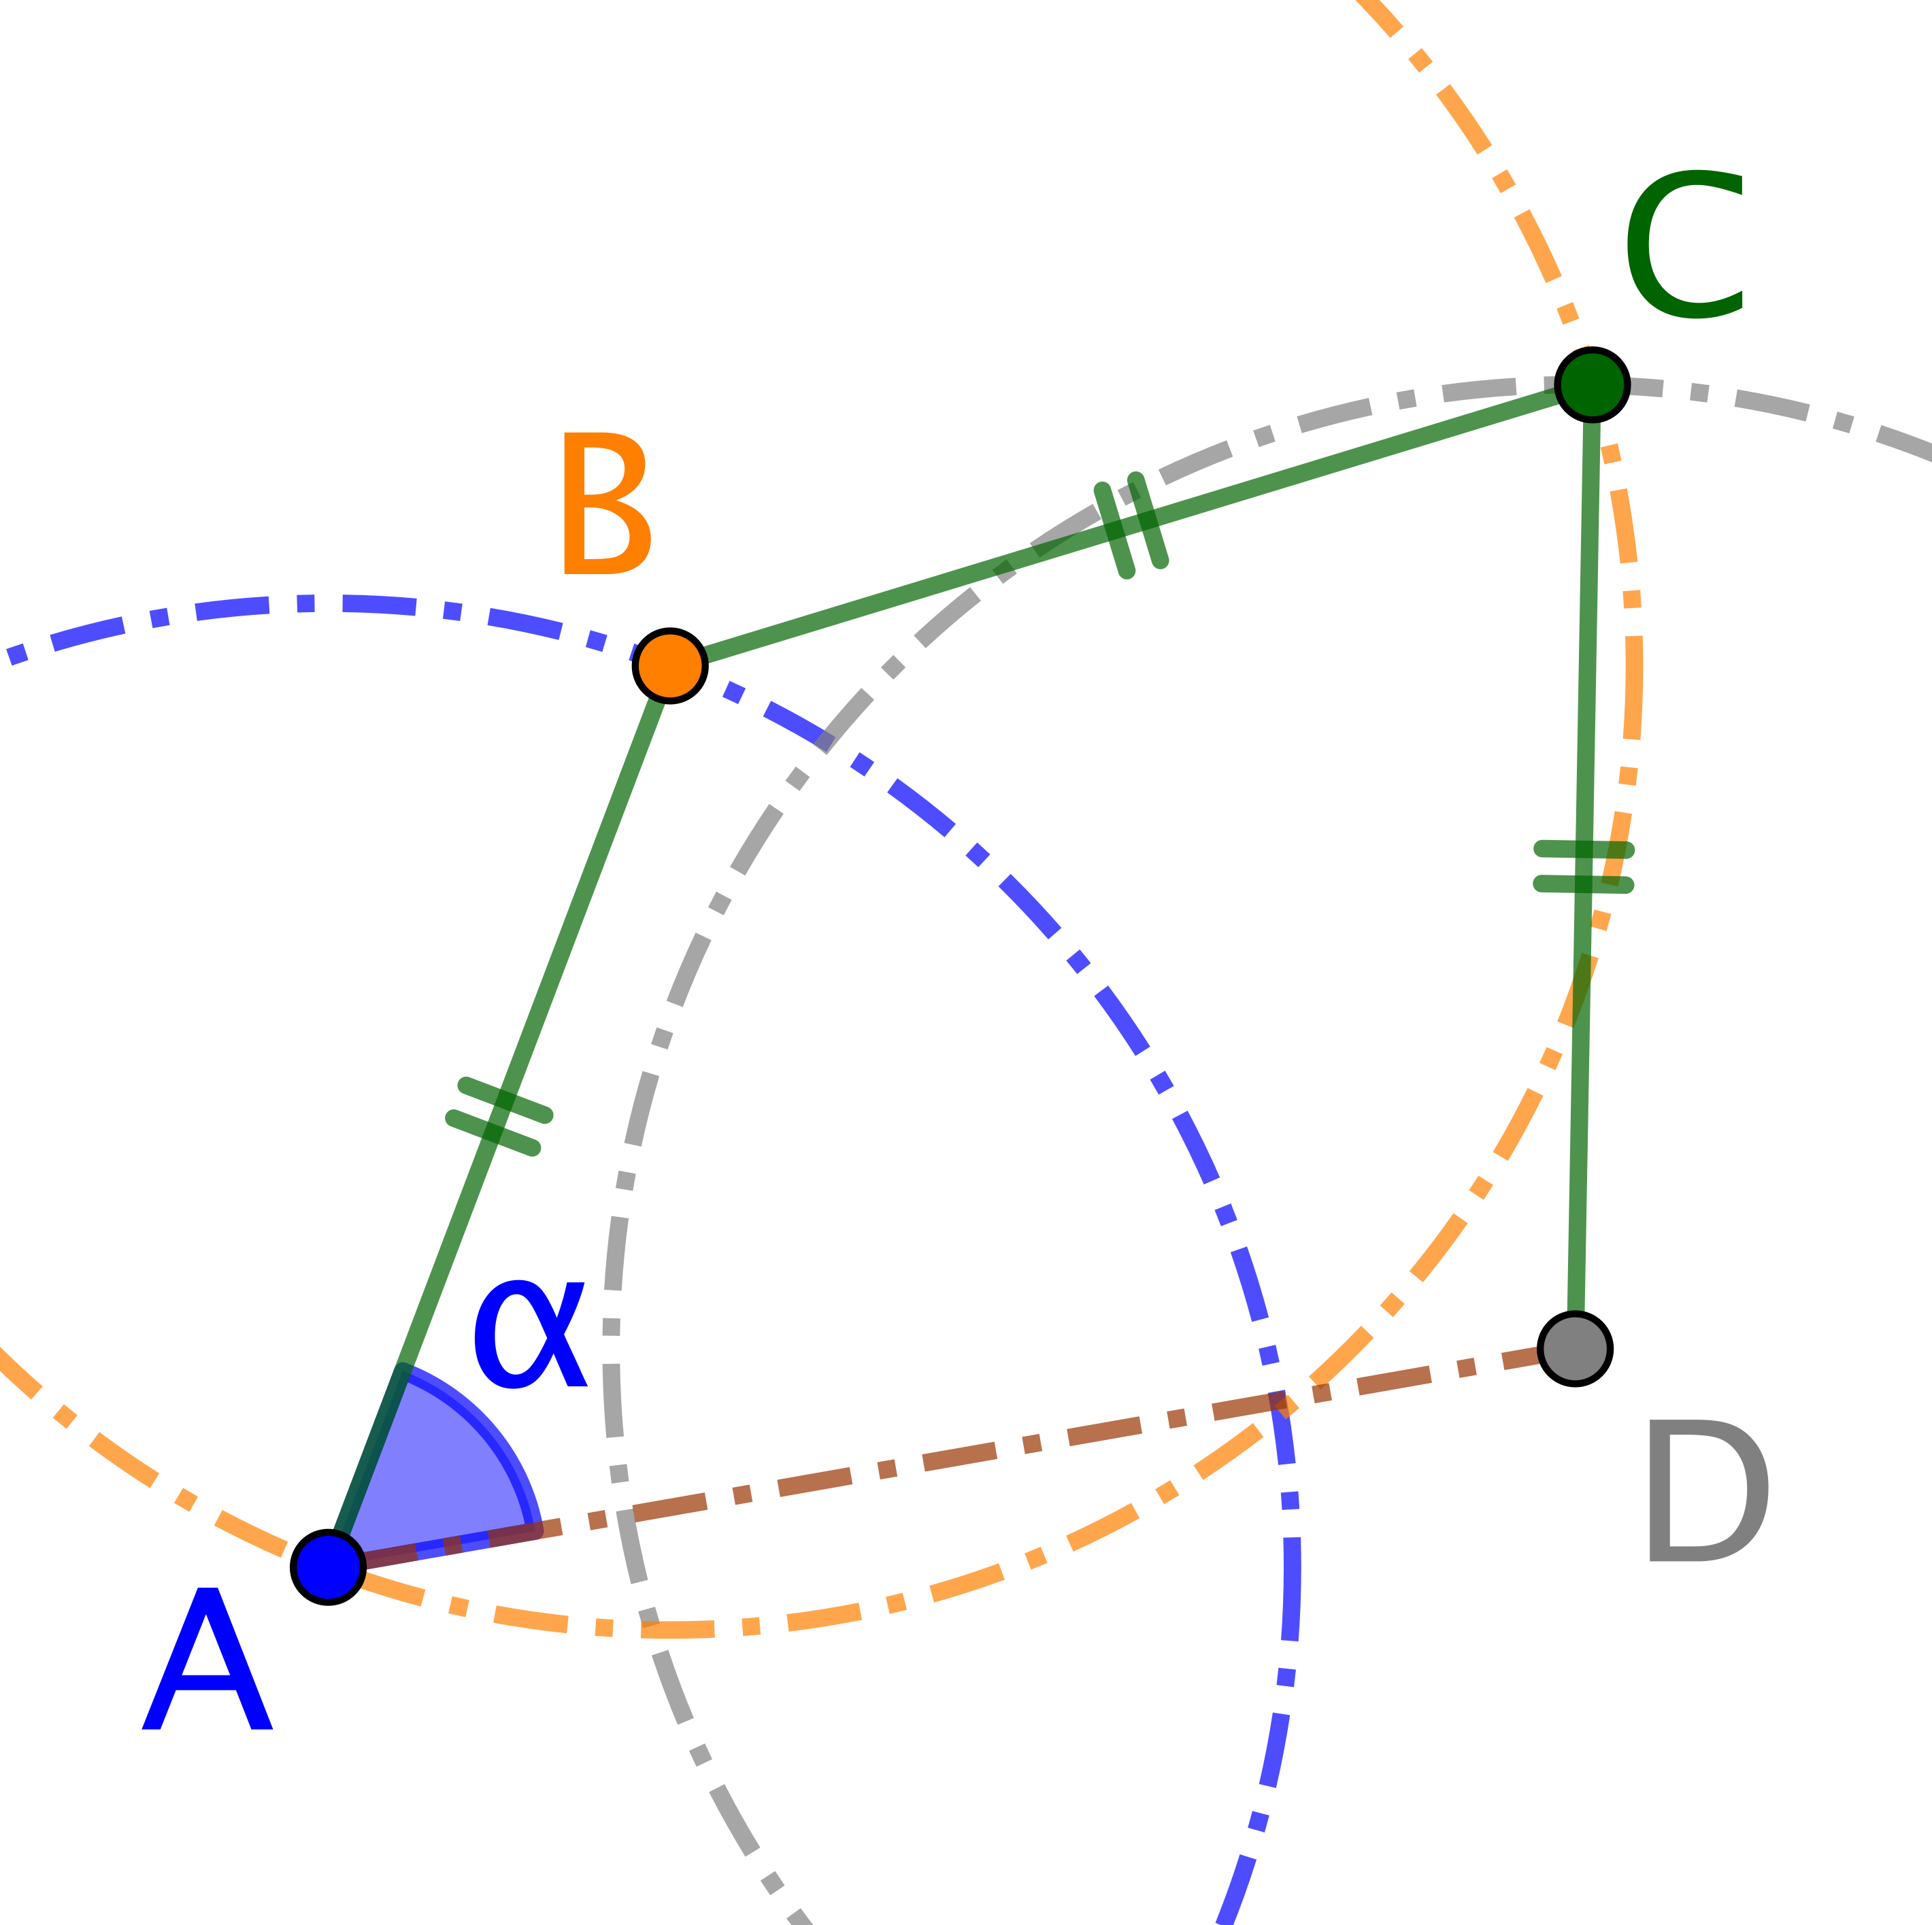
\includegraphics[scale=.4]{content/polygon/sol-must-be/2-eq-angles-circle.png}
	\end{center}

	Cherchons donc à exprimer $\area{ABCD}$ en fonction de $\alpha = \anglein{DAB}$, cet angle permettant de repérer le point mobile $B$.
	%
	\begin{itemize}
	    \item Nous avons $\alpha \in \intervalO{0}{\pi}$ et $\gamma \in \intervalO{0}{\pi}$.


	    \item Le théorème d'Al-Kashi donne
	    $BD^2 = c^2 + d^2 - 2 c d \cos \alpha$ dans le triangle $ABD$,
	    ainsi que
	    $BD^2 = 2 c^2 - 2 c^2 \cos \gamma$ dans le triangle $BCD$.
	    Donc,
	    $2 \cos \gamma = 1 - k^2 + 2 k \cos \alpha$ où l'on a posé $k = \frac{d}{c}$.
	    Notons que l'inégalité triangulaire donne $d < 3 c$, puis $0 < k < 3$.


	    \item La formule trigonométrique de l'aire d'un triangle donne
	    $\area{ABD} = \num{.5} c d \sin \alpha$
	    et
	    $\area{BCD} = \num{.5} c^2 \sin \gamma$,
	   	puis
	    $\area{ABCD} = \num{.5} c^2 ( k \sin \alpha + \sin \gamma )$,
	    de sorte que
    	$\area{ABCD} = \num{.5} c^2 f(\alpha)$
    	en posant 
    	$f(\alpha) = k \sin \alpha + \sqrt{1 - \num{.25} ( 1 - k^2 + 2 k \cos \alpha)^2}$,
	    car 
	    $\sin \gamma = \sqrt{1 - \cos^2 \gamma}$.


	    \item Passons à l'étude de $\sder{f}{1}(\alpha) = 0$, en nous souvenant que nous n'avons pas besoin d'atteindre le maximum de $f$, mais juste de pouvoir faire augmenter localement $f(\alpha)$. 
	    Dans les implications suivantes, nous avons posé 
	    $\onelist{S} = \sin \alpha$ et $\onelist{C} = \cos \alpha$.
	    
	    \begin{stepcalc}[style=ar*, ope={\implies[d'où]}]
	        \sder{f}{1}(\alpha) = 0
	    \explnext{}
	        k \onelist{C}
	        +
	        \dfrac{ k \onelist{S} ( 1 - k^2 + 2 k \onelist{C}) }{ 2 \sqrt{1 -  \num{.25} ( 1 - k^2 + 2 k \onelist{C})^2} }
	        =
	        0
	    \explnext{}
	        \onelist{S} ( 1 - k^2 + 2 k \onelist{C}) 
	        =
	        - 2 \onelist{C} \sqrt{1 - \num{.25} ( 1 - k^2 + 2 k \onelist{C})^2}
	    \explnext{}
	        \onelist{S}^2 ( 1 - k^2 + 2 k \onelist{C})^2
	        =
	        4 \onelist{C}^2 \big( 1 - \num{.25} ( 1 - k^2 + 2 k \onelist{C})^2 \big)
	    \explnext{}
	        ( 1 - k^2 + 2 k \onelist{C})^2 (\onelist{S}^2 + \onelist{C}^2)
	        =
	        4 \onelist{C}^2
	    \explnext*{$\onelist{C}^2 + \onelist{S}^2 = 1$}{}
	        ( 1 - k^2 + 2 k \onelist{C})^2 - 4 \onelist{C}^2 = 0
	    \explnext{}
	        ( 1 - k^2 + 2 k \onelist{C} - 2 \onelist{C} )
	        \,
	        ( 1 - k^2 + 2 k \onelist{C} + 2 \onelist{C} )
	        = 0
	    \explnext{}
	        (1 - k) ( 1 + k - 2 \onelist{C} )
	        \,
	        (1 + k) ( 1 - k + 2 \onelist{C} ) = 0
	    \explnext*{$k > 0$}{}
	        k = 1
	        \,\, \text{ou} \,\,
	        \onelist{C} \in \setgene{ \frac{k - 1}{2} , \frac{k + 1}{2} }
	    \end{stepcalc}


	    \item $k = 1$ signifie que $ABCD$ est un losange, non rectangle, car $\anglein{ABC} \neq \anglein{BCD}$.
	    Dans ce cas, en bougeant un peu le sommet $B$ parallèlement à $(AD)$, tout en faisant
	    augmenter $\alpha$ légèrement si $\alpha \in \intervalO{0}{\frac{\pi}{2}}$,
	    ou
	    diminuer $\alpha$ légèrement si $\alpha \in \intervalO{\frac{\pi}{2}}{\pi}$,%
	    \footnote{
	        $B$ se déplace vers la gauche dans notre cas.
	    }
	    nous obtenons un parallélogramme de même aire, mais de périmètre diminué.%
	    \footnote{
	        Si besoin, se reporter à la preuve du fait \ref{iso-para}.
	    }
	    On obtient au final un \ngone\ convexe $\primeit{\setproba{P}}$ tel que
		$\perim{\primeit{\setproba{P}}} < \perim{\setproba{P}}$
		et
		$\area{\primeit{\setproba{P}}} = \area{\setproba{P}}$,
		qu'il suffit d'agrandir pour conclure.


	    \item Pour $k \neq 1$ et $\onelist{C} = \frac{k - 1}{2}$,
	    nous avons $2\cos \alpha = k - 1$, 
	    puis 
	    $2 \cos \gamma = 1 - k^2 + k(k - 1) = 1 - k$,
	    soit
	    $\cos \gamma = - \cos \alpha$ qui fournit
	    $\gamma = \pi - \alpha$, en se souvenant que $(\alpha , \gamma) \in \intervalO{0}{\pi}^2$.
	    Notons que $\alpha \neq \frac{\pi}{2}$ et $\gamma \neq \frac{\pi}{2}$, car $k \neq 1$.
	    %
	    
	    
	    XXX


	    \item Pour $k \neq 1$ et $\onelist{C} = \frac{k + 1}{2}$,
	    comme au début du point précédent,
	    nous avons $\cos \gamma = \cos \alpha$, puis $\gamma = \alpha$ avec $(\alpha , \gamma) \in \intervalO{0}{\pi}^2$.
	    Notons qu'ici $0 < k < 1$, puis $(\alpha , \gamma) \in \intervalO{0}{\frac{\pi}{3}}^2$.
	    Dès lors, les monotonies de $\sin$ et $\cos$ sur $\intervalO{0}{\frac{\pi}{3}}$, combinées à $1 - k^2 + 2 k \cos \alpha \geq 0$, impliquent la stricte croissance de $f$ sur $\intervalO{0}{\frac{\pi}{3}}$.%
	    \footnote{
	    	Nous utilisons la composition de fonctions monotones, ce qui n'est pas toujours faisable.
	    }
	    Il suffit donc d'augmenter légèrement la valeur de  $\alpha$.
	\end{itemize}
	
	\null\vspace{-6ex}
\end{proof}


\begin{remark}
    Ce qui précède donne envie de faire appel à la méthode des extrema liés pour plus d'élégance dans les calculs.
    Étudions donc les extrema de
	$f(\alpha , \gamma) = k \sin \alpha + \sin \gamma$
	sur $\intervalO{0}{\pi}^2$ sous la contrainte
	$g(\alpha , \gamma) = 0$
	avec
	$g(\alpha , \gamma) = 1 - k^2 + 2 k \cos \alpha - 2 \cos \gamma$.
	%
    Si un extremum existe, alors nous avons $\lambda \in \RR$ tel que
    $\pder[i]{f}{\alpha}{1} = \lambda \pder[i]{g}{\alpha}{1}$
	et
    $\pder[i]{f}{\gamma}{1} = \lambda \pder[i]{g}{\gamma}{1}$,
	de sorte que
	$k \cos \alpha = - 2 k \lambda \sin \alpha$,
	soit
	$\cos \alpha = - 2 \lambda \sin \alpha$,
	et aussi
	$\cos \gamma = 2 \lambda \sin \gamma$.
	Nous avons alors les deux alternatives suivantes qui rejoignent les arguments de la preuve précédente.
	%
	\begin{enumerate}
	    \item Si $\lambda = 0$,
	    alors
	    $\alpha = \gamma = \frac{\pi}{2}$, puis $k = 1$. 

	    \item Si $\lambda \neq 0$,
	    alors
	    $\cos \alpha \sin \gamma = - \cos \gamma \sin \alpha$,
	    puis
	    $\sin (\alpha + \gamma) = 0$,
	    et
	    $\gamma = \pi - \alpha$.
	\end{enumerate}
\end{remark}


\begin{remark}
	Une démonstration géométrique du fait \ref{must-be-iso} est possible via un résultat attribué à Zénodore%
	\footnote{
	    La preuve du résultat de Zénodore est un peu fastidieuse.
	}
	sur la maximisation de l'aire totale de deux triangles isocèles de bases fixées, et de périmètre total constant:
	ce résultat affirme que les deux triangles doivent avoir des angles en leur sommet principal de même mesure.
	Malheureusement, cette preuve échoue lors de la disparition d'un sommet en choisissant la paire optimale de triangles isocèles pour construire un nouveau \ngone\ \focus{plus gros}.
\end{remark}


% ----------------------- %


\begin{fact} \label{must-be-reg}
	Si un \ngone\ $\setproba{P}$ n'est pas un \nreg\ convexe,
	alors il existe un \ngone\ convexe $\primeit{\setproba{P}}$ tel que
	$\perim{\primeit{\setproba{P}}} = \perim{\setproba{P}}$
	et
	$\area{\primeit{\setproba{P}}} > \area{\setproba{P}}$.
\end{fact}


\begin{proof}
	Il suffit d'utiliser les faits \ref{must-be-conv}, \ref{must-be-equi} et \ref{must-be-iso}.
\end{proof}


% ----------------------- %


Pour en finir avec le problème d'isopérimétrie polygonal, nous aurons besoin du fait suivant.


\begin{fact} \label{nregs-sorting}
	Si $\setproba*{R}{1}$ et $\setproba*{R}{2}$ sont respectivement un \xgone{k_1} et un \xgone{k_2}, tous les deux réguliers convexes, avec 
	$k_1 < k_2$ et $\perim{\setproba*{R}{1}} = \perim{\setproba*{R}{2}}$,
	alors
	$\area{\setproba*{R}{1}} < \area{\setproba*{R}{2}}$.
\end{fact}


\begin{proof}
    Il est connu, et facile à démontrer, qu'un \nreg\ convexe $\setproba{R}$ vérifie
    $\perim{\setproba{R}} = 2 n \sin (\frac{\pi}{n}) \rho$
    et
	$\area{\setproba{R}} = n \sin (\frac{\pi}{n})  \cos (\frac{\pi}{n}) \rho^2$
	où $\rho$ désigne le rayon du cercle circonscrit à $\setproba{R}$.
	Ceci donne 
	$\area{\setproba{R}} = \frac{\perim{\setproba{R}}^2}{4 n \tan (\frac{\pi}{n})}$,
	puis amène à justifier que 
	$k_1 \tan (\frac{\pi}{k_1}) > k_2 \tan (\frac{\pi}{k_2})$,
	c'est-à-dire que la suite $\big( k \tan (\frac{\pi}{k}) \big)_{k \in \NN_{\geq 3}}$ est strictement décroissante.
	
	
	XXXX
\end{proof}




%\subsection{Théorème d'isopérimétrie polygonal}
%\begin{fact}
    Soit $n \in \NN_{\geq3}$ un naturel fixé.
    Parmi les \ngones\ de périmètre fixé, non nul,
    le \nreg\ convexe est le seul à maximiser l'aire.
\end{fact}


\begin{proof}
    Tout a été fait, il ne reste plus qu'à assembler les arguments.
    %
    \begin{enumerate}
        \item Le cas $n = 3$ correspond au fait \ref{iso-tri}.
        
        \item Le cas $n = 4$ a été établi dans le fait \ref{quadri}.
        
        \item Pour $n \geq 5$, il suffit de se rappeler des faits suivants où $\ell \in \RRsp$.
        %
        \begin{itemize}
            \item D'après le fait \ref{at-least-one-ngone-convex}, il existe, au moins, un \ngone\ convexe maximisant l'aire parmi les \ngones\ convexes de périmètre, ou de longueur, fixé.

            \item Selon le fait \ref{must-be-reg}, un \ngone\ \focus{maximal} doit être, a minima, régulier et convexe.

            \item Soit $\setproba{M}$ un \ngone\ convexe maximisant l'aire parmi les \ngones\ convexes de périmètre fixé.
            Si $\setproba{M}$ n'est pas régulier, alors soit il n'est pas équilatéral, soit il est équilatéral, mais pas équiangle.
            Or, ces alternatives sont impossibles d'après les faits \ref{must-be-equi} et \ref{must-be-iso}.

            \item Pour un périmètre donné, non nul, il n'existe qu'un seul \nreg\ convexe ayant ce périmètre.
        \end{itemize} 
	
	\null\vspace{-6ex}
    \end{enumerate}
\end{proof}

\bigskip
\hfill {\small\itshape\bfseries Ici s'achève notre joli voyage}.

\end{document}
